% p + p -> pi+ pi- e+ e- Analysis Report
% Build: cd docs/latex && pdflatex report && pdflatex report
% Figures: macros/rep_banana.C (beta_new vs q*p), tables: macros/rep_stats.C
\documentclass[11pt,a4paper]{article}
\usepackage[T1]{fontenc}
\usepackage[utf8]{inputenc}
\usepackage{lmodern}
\usepackage[margin=2.2cm]{geometry}
\usepackage{amsmath}
\usepackage{graphicx}
\usepackage{booktabs}
\usepackage{tabularx}
\usepackage{longtable}
\usepackage{xcolor}
\usepackage{caption}
\usepackage{float}
\usepackage{microtype}
\usepackage{listings}
\usepackage{xspace}
\usepackage[colorlinks=true,linkcolor=blue!50!black,urlcolor=blue!50!black,citecolor=blue!50!black]{hyperref}

\captionsetup{font=small,labelfont=bf,margin=0.5cm}
\setlength{\parskip}{0.45em}
\setlength{\emergencystretch}{3em}
\setlength{\parindent}{0pt}
\renewcommand{\arraystretch}{1.15}
\newcolumntype{L}{>{\raggedright\arraybackslash}X}

\lstset{basicstyle=\ttfamily\small,columns=fullflexible,keepspaces=true,frame=single,
        framerule=0.3pt,rulecolor=\color{black!30},backgroundcolor=\color{black!3},
        xleftmargin=0.5em,xrightmargin=0.5em,aboveskip=0.6em,belowskip=0.6em}

% physics shorthands
\newcommand{\pip}{\ensuremath{\pi^{+}}\xspace}
\newcommand{\pim}{\ensuremath{\pi^{-}}\xspace}
\newcommand{\piz}{\ensuremath{\pi^{0}}\xspace}
\newcommand{\ee}{\ensuremath{e^{+}e^{-}}\xspace}
\newcommand{\pipi}{\ensuremath{\pi^{+}\pi^{-}}\xspace}
\newcommand{\ppee}{\ensuremath{\pi^{+}\pi^{-}e^{+}e^{-}}\xspace}
\newcommand{\Mfour}{\ensuremath{M(\pi^{+}\pi^{-}e^{+}e^{-})}\xspace}
\newcommand{\Mee}{\ensuremath{M(e^{+}e^{-})}\xspace}
\newcommand{\Mpipi}{\ensuremath{M(\pi^{+}\pi^{-})}\xspace}
\newcommand{\betanew}{\ensuremath{\beta_{\mathrm{new}}}\xspace}
\newcommand{\nbinv}{\ensuremath{\mathrm{nb}^{-1}}\xspace}
\newcommand{\GeVc}{\ensuremath{\mathrm{GeV}/c}\xspace}
\newcommand{\MeVc}{\ensuremath{\mathrm{MeV}/c}\xspace}
\newcommand{\GeVcc}{\ensuremath{\mathrm{GeV}/c^{2}}\xspace}
\newcommand{\MeVcc}{\ensuremath{\mathrm{MeV}/c^{2}}\xspace}
\newcommand{\Lsim}{\ensuremath{L_{\mathrm{sim}}}\xspace}
\newcommand{\Ldata}{\ensuremath{L_{\mathrm{data}}}\xspace}
\newcommand{\code}[1]{\texttt{\detokenize{#1}}}
\newcommand{\chem}[1]{\ensuremath{\mathrm{#1}}}
\newcommand{\notebox}[1]{\par\noindent\colorbox{orange!10}{\parbox{\dimexpr\linewidth-2\fboxsep\relax}{#1}}\par}
\newcommand{\tipbox}[1]{\par\noindent\colorbox{blue!6}{\parbox{\dimexpr\linewidth-2\fboxsep\relax}{#1}}\par}

\title{\Large $p + p \to \pi^{+}\pi^{-}e^{+}e^{-}$ Analysis Report\\[0.4em]
       \normalsize HADES, p+p at $T = 4.5$\,GeV (feb22 beam time)\\
       Part I: the simulation basis}
\author{W.~Przygoda}
\date{Draft of 13 November 2026}

\begin{document}
\maketitle

\notebox{\textbf{Status of this draft.}
Part~I uses simulation only. Two inputs are still provisional and are kept as parameters:
(i) the integrated luminosity of the data, $\Ldata = 6080.5\,\nbinv$, taken from the
producers' note and not yet confirmed by the luminosity analysis;
(ii) the physics weights of the simulated $\eta$ decays (Sect.~\ref{sec:etagen}). The
generator's $\eta\to\ppee$ has a non-QED $\Mee$ distribution; it is now corrected by weights
(main variant V3), as are the Dalitz plot of $\eta\to\pipi\piz$ and the pion form factor of
$\eta\to\pipi\gamma$. Numbers marked ``(pre-rw)'' are before these weights.}

\tableofcontents

{\footnotesize
\setlength{\tabcolsep}{4pt}
\renewcommand{\arraystretch}{1.06}
\begin{longtable}{@{}>{\raggedright\arraybackslash}p{3.0cm} >{\raggedright\arraybackslash}p{\dimexpr\textwidth-3.0cm-2.2cm-4\tabcolsep\relax} >{\raggedright\arraybackslash}p{2.2cm}@{}}
\caption{\textbf{Notation and abbreviations.} Last column: where the item is defined in detail.}
\label{tab:notation}\\
\toprule
Symbol & Meaning & Details \\
\midrule
\endfirsthead
\toprule
Symbol & Meaning & Details \\
\midrule
\endhead
\bottomrule
\endfoot
\multicolumn{3}{@{}l}{\textbf{Programs and samples}} \\
SMASH, PLUTO & event generator of p+p collisions; decay generator used by the converter & \S\ref{sec:samples} \\
converter & \code{convert-smash}: SMASH output $\to$ HGeant input, forces decays in the lepton and $\eta$ sets & Tab.~\ref{tab:sets} \\
HGeant, DST & GEANT3-based HADES detector simulation; reconstructed data & Tab.~\ref{tab:prod} \\
PAT, FAT & PostDST Analysis Tool (hypotheses, PID, relative time, ranking); Final Analysis Tool (selection, kinematics, weights) & \S\ref{sec:ana} \\
std, lep, $\eta$ set & simulation sets: natural decays; every \piz, $\eta$, $\rho^0$, $\omega$, $\phi$ forced into dileptons; every $\eta$ forced into \ppee or \pipi X17 & Tab.~\ref{tab:sets} \\
$N$, $b_{\max}$, $T$ & events per set ($10^{10}$); largest impact parameter (1.2\,fm); beam kinetic energy & Tab.~\ref{tab:norm} \\
\Lsim, \Ldata & luminosity of one simulated set (221.05\,\nbinv); of the data (6080.5\,\nbinv, not confirmed) & Tab.~\ref{tab:norm} \\
row & one combination of tracks of a hypothesis; an event can give several rows & \S\ref{sec:ana} \\
event group & the adjacent rows of one event (used for the statistical errors) & \S\ref{sec:tech} \\
isBest & PAT ranking of the combinations of an event: 1 best, 0 others; ``all combinations'' = isBest $\ge0$ & \S\ref{sec:ana} \\
PT3, \code{trigbit} & the physics trigger of this analysis; trigger word (PT3 = bit 8192; simulation 12288) & \S\ref{sec:tech} \\
``pre'' & base selection: isBest $\ge0$, vertex $z>-500$\,mm, PT3, vertex $z>-160$\,mm, corrected momenta & \S\ref{sec:sel} \\
\midrule
\multicolumn{3}{@{}l}{\textbf{Generator truth, classes and weights}} \\
\code{geninfo}, \code{geninfo1}, \code{geninfo2} & generator codes of a GEANT track: decay code, code of the direct parent, counter of the decay in the event & \S\ref{sec:float}, \S\ref{sec:key} \\
forced decay & a decay chosen by the converter instead of the natural one, with a stored weight $w$ & Tab.~\ref{tab:forced} \\
$w$, $W$ & generator weight stored on a track; physical weight of a row & \S\ref{sec:weights} \\
rules v1, v2 & weight rules; v2 uses the exact HGeant branching ratios of the card \code{ETA} & \S\ref{sec:hgeanteta} \\
mode A, B & ownership of row types between the sets (A default) & \S\ref{sec:weights} \\
classes 0--8 & four-particle truth class (\code{sim_cls}); signal classes 2--6 & Tab.~\ref{tab:classes} \\
L0--L11, P0--P9 & lepton-pair and pion-pair truth classes & Tab.~\ref{tab:classes} \\
T1--T4 & templates: signal, physical background, fake lepton, leptons from two sources & Tab.~\ref{tab:classes} \\
$G_\eta$, $G_{\pi^0\mathrm{D}}$, $G_{\mathrm{conv}}$, $G_{\mathrm{vec}}$, $G_{\mathrm{oth}}$ & groups of T2 by the source of the pair and the pions; multi-pion = $G_{\pi^0\mathrm{D}}+G_{\mathrm{conv}}+G_{\mathrm{vec}}$ & Tab.~\ref{tab:s5defs} \\
ghost & reconstructed track flagged as not matching one GEANT particle (\code{sim_isghost}) & Tab.~\ref{tab:classes} \\
pre-rw, V0--V4 & before the physics reweighting of the $\eta$ decays; its model variants (V3 main) & \S\ref{sec:etagen} \\
\midrule
\multicolumn{3}{@{}l}{\textbf{Cross sections and statistics}} \\
$\sigma_{\mathrm{prod}}$ & production cross section in SMASH: mean number per collision $\times\,\pi b_{\max}^2$ & Tab.~\ref{tab:smashprod} \\
BR & branching ratio (PDG unless stated) & Tab.~\ref{tab:forced}, \ref{tab:hgeant} \\
$\varepsilon$, $N_{\mathrm{gen}}$ & rows after ``pre'' per generated decay; number of generated decays & Tab.~\ref{tab:cls} \\
$\sigma_{\mathrm{vis}}$, $\sigma$ & visible cross section $\sum W/\Lsim$ of rows; $=\sigma_{\mathrm{prod}}\times\mathrm{BR}\times\varepsilon$ & \S\ref{sec:xsec} \\
$N_{\mathrm{eff}}$ & effective number of rows, $(\sum W)^2/\mathrm{Var}$ & \S\ref{sec:simres} \\
CB, $k$ & combinatorial background of the data, $2\sqrt{N_{++}N_{--}}$ times $k$ (absent in simulation) & \S\ref{sec:ana} \\
\midrule
\multicolumn{3}{@{}l}{\textbf{Particle identification}} \\
$\betanew$ & velocity from the relative times of flight of the tracks of a hypothesis & \S\ref{sec:pid} \\
charge $\times$ momentum & horizontal axis of the PID plots (negative for negative tracks) & Fig.~\ref{fig:banana} \\
$n\sigma$ cut, v1, v6 & PID polygon at $n$ standard deviations; experiment (v1) and simulation (v6) cut files & \S\ref{sec:pid} \\
ring, \code{kIsLepton} & RICH ring correlated with the track; PAT puts such tracks into lepton slots & \S\ref{sec:pid} \\
\midrule
\multicolumn{3}{@{}l}{\textbf{Kinematics and cuts}} \\
\Mfour, \Mee, \Mpipi & invariant masses of \ppee, of the \ee pair, of the \pipi pair & \\
$\mathrm{MM}_4$ & missing mass of \ppee: mass of (beam + target $-$ \ppee) four-momenta; for $pp\to pp\eta$ it is $M(pp)$ & Tab.~\ref{tab:cuts} \\
$p_{T,4}$, $y_4$ & transverse momentum (lab) and rapidity (beam--target c.m.) of \ppee & Tab.~\ref{tab:cuts} \\
OA & opening angle between $e^+$ and $e^-$ (lab) & Tab.~\ref{tab:cuts} \\
$\alpha_{\mathrm{lab}}$ & angle between the \pipi and \ee momenta (lab) & Tab.~\ref{tab:cuts} \\
$\alpha_\eta$ & angle between \pipi and \ee in the rest frame of a hypothetical $\eta$ (measured \ppee momentum, mass $m_\eta$) & Tab.~\ref{tab:cuts} \\
$\Delta z_\pi$ & largest $|z_{\mathrm{track}}-z_{\mathrm{vertex}}|$ of the two pions & Tab.~\ref{tab:cuts} \\
pions in vertex fit & both pion tracks used in the event-vertex fit (\code{isUsedVertex}) & Tab.~\ref{tab:cuts} \\
named selections & pre, pre+OA$>2$, slides, old code, peak nominal, bump nominal & Tab.~\ref{tab:presets} \\
bump, peak & $\eta\to\pipi\piz$ seen below $m_\eta$; $\eta$ at $m_\eta$ (direct decay or conversion) & \S\ref{sec:scope} \\
peak / bump window & $0.5333\le\Mfour<0.5587$ / $0.4576\le\Mfour<0.5255$\,\GeVcc (simulation) & Tab.~\ref{tab:s5defs} \\
\midrule
\multicolumn{3}{@{}l}{\textbf{Optimisation and blind test (Section~\ref{sec:simres})}} \\
$S$, $B$, $P$ & signal rows, other T1+T2 rows of a window, purity $S/(S+B)$ & \S\ref{sec:s5spec} \\
$F$, $F_{\mathrm{best}}$ & figure of merit $S/\sqrt{S+B}$; its maximum over the scanned cuts & \S\ref{sec:s5opt} \\
PEAK, DIRECT, BUMP & optimisation targets: classes 4+5, class 5, classes 2+3 in their window & \S\ref{sec:s5opt} \\
plateau, freeze rule & cuts with $F\ge0.95\,F_{\mathrm{best}}$; the rule that picks the frozen cut & \S\ref{sec:s5opt} \\
half A, B & simulated events split by event-group number (even/odd): templates / pseudo-data & \S\ref{sec:s5blind} \\
toy, $\mu$ & one pseudo-data set; the expected (true) yield of half B & \S\ref{sec:s5blind} \\
bias, pull, coverage & mean (extracted $-\mu$); (extracted $-\mu$)/quoted error; fraction of toys with $|Y-\mu|\le$ error & Tab.~\ref{tab:s5blind} \\
M1--M3c, B1--B4, D5 & extraction methods for the peak, the bump, the direct decay & \S\ref{sec:s5blind} \\
X1--X5 & X17 estimators & \S\ref{sec:s5blind} \\
UL, $\mathrm{UL}_{\mathrm{stat}}$, $s_1$ & expected 90\,\% CL limit with / without the simulation error of $B$; X17 rows per unit BR & Eq.~(\ref{eq:s5ul}) \\
\end{longtable}
}

%======================================================================
\section{Scope}
\label{sec:scope}
%======================================================================
The analysis looks for the $\eta$ meson in the final state $\ppee$ of p+p collisions at
$T = 4.5$\,GeV. Two structures are expected in the invariant mass $\Mfour$:
\begin{itemize}
\item the \textbf{peak} at $m_\eta$ from the decay $\eta\to\ppee$, and from
      $\eta\to\pipi\gamma$ when the photon converts into an \ee pair in the detector;
\item the \textbf{bump} below $m_\eta$ from $\eta\to\pipi\piz$ followed by the Dalitz decay
      $\piz\to\ee\gamma$ (or by a photon conversion), when the photon is not detected.
\end{itemize}
The bump is much larger than the peak and has a known branching ratio, so it can serve as a
reference. The \ee pairs of the peak are also the place to search for a hypothetical X17
boson ($\eta\to\pipi X17$, $X17\to\ee$).

This first part documents the simulation used for the analysis: the samples, their
statistics and normalisation, the weights, several technical pitfalls met on the way, and a
short description of the selection. The data analysis and the comparisons follow in later
parts (Sect.~\ref{sec:next}).

%======================================================================
\section{Simulation samples}
\label{sec:samples}
%======================================================================

\subsection{Event generator and the three sets}
All simulated events come from one SMASH run: p+p at $T = 4.5$\,GeV, SMASH-3.0, collider
mode, impact parameter sampled uniformly in the area in $[0, 1.2]$\,fm. Every sampled event
is kept, including the 4.3\,\% without any interaction. The converter (\code{convert-smash})
turns the SMASH output into HGeant input; it was run three times on the \emph{same}
$10^{10}$ events, with different treatment of some particles (Table~\ref{tab:sets}).
This was verified: the converted files of the three sets are identical event by event apart
from the forced particles, and the reconstructed rows of different sets contain the same
generator pions (Sect.~\ref{sec:rotation}). The three sets therefore describe the same
collisions; only the detector simulation (HGeant) is independent in each set.

\begin{table}[H]
\centering
\caption{The three SMASH simulation sets. ``Forced'' means that the converter (with PLUTO)
replaced the natural decay of every such particle by the listed channel and stored a weight
on its products. Weight 0 in the file means ``not weighted'' (natural probability).}
\label{tab:sets}
\begin{tabularx}{\textwidth}{@{}>{\raggedright\arraybackslash}p{1.9cm} >{\raggedright\arraybackslash}p{5.7cm} L >{\raggedright\arraybackslash}p{2.9cm}@{}}
\toprule
Set & Converter run & What is changed & Weight stored on the products \\
\midrule
standard (\code{std}) & 2026-05-18, \code{-u 0}, no PLUTO &
  nothing; \piz and $\eta$ decay in HGeant; SMASH resonance decays ($\rho,\omega,\phi$) are
  only flagged in the generator code & 0 for every particle \\
lepton (\code{lep}) & 2026-02-11, PLUTO,\newline \code{database_decays_leptons.dat} &
  every \piz, $\eta$, $\rho^0$, $\omega$, $\phi$ forced into a dilepton channel
  (Table~\ref{tab:forced}) & $w = n_{\mathrm{ch}}\times\mathrm{BR}$ on the forced-decay products \\
$\eta$ (\code{eta}) & 2026-06-03, PLUTO,\newline \code{database_decays_eta.dat} &
  every $\eta$ forced: 50\,\% $\eta\to\ppee$, 50\,\% $\eta\to X17\,\pipi$, $X17\to\ee$
  ($m_{X17}=17$\,\MeVcc) & $w = 2$ on the four products \\
\bottomrule
\end{tabularx}
\end{table}

\begin{table}[H]
\centering
\caption{Normalisation, common to the three sets.}
\label{tab:norm}
\begin{tabularx}{\textwidth}{@{}l L@{}}
\toprule
Events per set & $N = 10^{10}$ (100\,000 files $\times$ 100\,000 events) \\
Area per event & $\pi b_{\max}^2 / N = 45.239\,\mathrm{mb}/10^{10} = 4.5239\times10^{-3}$\,nb \\
Integrated luminosity per set & $\Lsim = N/(\pi b_{\max}^2) = 221.05\,\nbinv$ \\
SMASH cross sections (for orientation) & $\sigma_{\mathrm{tot}} = 43.29\pm0.03$\,mb,
   $\sigma_{\mathrm{el}} = 12.72\pm0.06$\,mb, $\sigma_{\mathrm{inel}} = 30.57\pm0.07$\,mb \\
Expected rows in data & $N_{\mathrm{data}} = (\Ldata/\Lsim)\,\sum W_{\mathrm{row}}$;
   for $\Ldata = 6080.5\,\nbinv$: 27.51 per unit weight \\
\bottomrule
\end{tabularx}
\end{table}

Because $\sigma_{\mathrm{tot}} < \pi b_{\max}^2$, the range of $b$ covers every SMASH
collision. The luminosity of a set does not depend on the SMASH cross sections; the
particle yields per collision do.

\subsection{Detector simulation and PAT production}
The three sets went through HGeant and the HADES reconstruction (DST production feb22,
\code{gen4}). The DSTs were processed with PAT (PostDST Analysis Tool) into the three
hypothesis trees of this analysis. Table~\ref{tab:prod} lists the production.

\begin{table}[H]
\centering
\caption{PAT production of the simulation (all three sets with the same frozen binary).}
\label{tab:prod}
\begin{tabularx}{\textwidth}{@{}l L@{}}
\toprule
PAT branch, commit & \code{pp45_sim_pippimepem}, \code{e674942} (binary built 2026-11-11 20:42) \\
Software & Hydra 2.7.6, ROOT 6.36.02 (Debian 12) \\
PID cut file & \code{pp45_pid_cuts_sim_betanew_v6.root}: p, \pip, \pim at $3\sigma$,
   $e^\pm$ at $5\sigma$ (Sect.~\ref{sec:pid}) \\
Hypotheses written & \code{PipPimEpEm_ID}, \code{PipPimEpEp_ID}, \code{PipPimEmEm_ID}
   (level after the PID cut) \\
DST input & \code{/lustre/hades/dstsim/feb22/p4500p/}\allowbreak\code{gen4/smash/smash_<set>/root/}, 100\,000
   files per set, all processed, $10^{10}$ events per set \\
Merged files & \code{ppee_std_all.root} (0.30\,GB), \code{ppee_lep_all.root} (10.0\,GB),
   \code{ppee_eta_all.root} (4.0\,GB) \\
\bottomrule
\end{tabularx}
\end{table}

\begin{table}[H]
\centering
\caption{Rows (combinations) and events of the PAT hypothesis trees. ``Events'' counts the
events with at least one row.}
\label{tab:patrows}
\begin{tabular}{@{}l rr rr rr@{}}
\toprule
 & \multicolumn{2}{c}{\code{PipPimEpEm_ID}} & \multicolumn{2}{c}{\code{PipPimEpEp_ID}} &
   \multicolumn{2}{c}{\code{PipPimEmEm_ID}} \\
Set & rows & events & rows & events & rows & events \\
\midrule
std & 238\,074 & 220\,532 & 1\,146 & 1\,066 & 4\,850 & 4\,455 \\
lep & 7\,622\,819 & 7\,035\,072 & 207\,380 & 197\,954 & 498\,807 & 469\,069 \\
eta & 3\,508\,574 & 2\,869\,528 & 14\,042 & 12\,391 & 54\,156 & 45\,879 \\
\bottomrule
\end{tabular}
\end{table}

\subsection{Analysis-framework processing and statistics}
The PAT trees are read by FAT (Final Analysis Tool, \code{main.cc}), which applies the
base selection of Sect.~\ref{sec:sel}, computes the kinematics and the truth classes, and
writes one row per combination into the ntuple \code{scan_nt}. Table~\ref{tab:fat} gives the
statistics after each step.

\begin{table}[H]
\centering
\caption{Statistics after the analysis framework. ``FAT rows'': $\mathrm{isBest}\ge0$,
vertex $z>-500$\,mm, PT3 trigger bit. ``Owned'': rows that this set provides in the
partition of Sect.~\ref{sec:weights} (mode A). $\sum W$: sum of the physical weights of the
owned rows with $z>-160$\,mm; $\sigma = \sum W/\Lsim$ is the visible cross section (Sect.~\ref{sec:xsec}) for producing such
a row (pre-rw for the $\eta$ set).}
\label{tab:fat}
\begin{tabular}{@{}l l r r r r r@{}}
\toprule
Set & Channel & PAT rows & FAT rows & $z>-160$ & owned & $\sigma$ [nb] \\
\midrule
std & \ppee        &   238\,074 &   230\,469 &   230\,115 &   115\,414 & 506.73 \\
    & $\pi^+\pi^-e^+e^+$ &  1\,146 &  1\,133 &  1\,132 &  1\,055 & 3.911 \\
    & $\pi^+\pi^-e^-e^-$ &  4\,850 &  4\,791 &  4\,777 &  4\,599 & 18.85 \\
\midrule
lep & \ppee        & 7\,622\,819 & 7\,441\,490 & 7\,432\,170 & 7\,082\,339 & 329.36 \\
    & $\pi^+\pi^-e^+e^+$ &   207\,380 &   205\,527 &   205\,288 &   159\,543 & 0.285 \\
    & $\pi^+\pi^-e^-e^-$ &   498\,807 &   495\,711 &   495\,101 &   328\,641 & 0.608 \\
\midrule
eta & \ppee        & 3\,508\,574 & 3\,366\,025 & 3\,357\,676 & 3\,180\,398 & 3.290 \\
    & $\pi^+\pi^-e^+e^+$ &    14\,042 &    13\,881 &    13\,856 &    13\,061 & 0.0134 \\
    & $\pi^+\pi^-e^-e^-$ &    54\,156 &    53\,628 &    53\,510 &    49\,892 & 0.0586 \\
\bottomrule
\end{tabular}
\end{table}

The large row counts of the lepton and $\eta$ sets do not mean large cross sections: each
of their rows carries a small weight. For example, the 7.08 million owned \ppee rows of the
lepton set add up to $\sum W = 72\,804$, the 115\,414 rows of the standard set to
$112\,014$. The statistical power of a weighted sample is set by its effective number of
rows, $(\sum W)^2/\sum W^2$, not by its row count.

\subsection{Weights}
\label{sec:weights}
Every row gets a physical weight $W$, so that $\sum W/\Lsim$ is a cross section and the
three sets can be added. The rules (version~2, \code{src/sim_truth.h}) are:
\begin{enumerate}
\item \textbf{Standard set.} $W=1$, with corrections of the HGeant branching ratios to PDG
      values for decays that HGeant performs (Table~\ref{tab:hgeant}). The largest correction
      is for $\eta\to\ee\gamma$: the HGeant configuration of this production sets its branching
      ratio to 8.8 times the PDG value (Sect.~\ref{sec:hgeanteta}), so an \ee pair from an $\eta$
      Dalitz decay gets the factor 0.114.
\item \textbf{Lepton set.} $W$ is the product of the weights of the \emph{distinct} forced
      decays found among the four tracks (Table~\ref{tab:forced}), with the PDG/database
      branching-ratio correction. A track from no forced decay contributes the factor 1.
      Two tracks belong to the same forced decay when their codes $(\code{geninfo},
      \code{geninfo2})$ agree (Sect.~\ref{sec:key}).
\item \textbf{$\eta$ set.} A row with the four products of one forced decay gets
      $W = 2\times\mathrm{BR}$: $\mathrm{BR}(\eta\to\ppee) = 2.68\times10^{-4}$ (PDG), and a
      hypothesis value for X17 (0 by default). Everything else in this set is the standard
      set without the natural $\eta$ decays.
\item \textbf{Ownership.} One row type must come from one set only. In mode~A (default) the
      lepton set provides every row with a forced-decay product of a \piz, $\eta$, $\rho^0$,
      $\omega$ or $\phi$, and the standard set drops such rows; the $\eta$ set provides every
      row with a product of a forced $\eta$ decay. Mode~B (variant) leaves the \piz and $\eta$
      Dalitz rows in the standard set.
\end{enumerate}

\begin{table}[H]
\centering
\caption{Forced decays of the lepton set. The converter picks one of the $n_{\mathrm{ch}}$
active channels of a mother with equal probability, so the stored weight is
$n_{\mathrm{ch}}\times\mathrm{BR}$.}
\label{tab:forced}
\begin{tabular}{@{}l c l l l l@{}}
\toprule
Decay & $n_{\mathrm{ch}}$ & BR (database) & stored $w$ & BR (PDG) & PDG/database \\
\midrule
$\piz\to\ee\gamma$          & 1 & $1.198\times10^{-2}$ & 0.01198 & $1.174\times10^{-2}$ & 0.980 \\
$\eta\to\ee\gamma$          & 1 & $0.6\times10^{-2}$ & 0.006 & $0.69\times10^{-2}$ & 1.15 \\
$\rho^0\to\ee$              & 1 & $4.48\times10^{-5}$ & $4.5\times10^{-5}$ & $4.72\times10^{-5}$ & 1.054 \\
$\omega\to\ee$              & 2 & $7.15\times10^{-5}$ & $1.43\times10^{-4}$ & $7.38\times10^{-5}$ & 1.032 \\
$\omega\to\piz\ee$          & 2 & $5.9\times10^{-4}$ & $1.18\times10^{-3}$ & $7.7\times10^{-4}$ & 1.305 \\
$\phi\to\ee$                & 1 & $2.99\times10^{-4}$ & $2.99\times10^{-4}$ & $2.979\times10^{-4}$ & 0.996 \\
\bottomrule
\end{tabular}
\end{table}

\begin{table}[H]
\centering
\caption{Decays of \piz and $\eta$ performed by HGeant, and the correction factors applied to
rows with such decays (rules v2). ``Card'': the branching ratios in percent set in the HGeant
configuration of this production (\piz: HGeant default, no card); HGeant normalises them to
their sum. The producers' measurement on $10^6$ events (used in rules v1) agrees with the
normalised card within 0.3--2.2 standard deviations. The two \pipi modes of the $\eta$ cannot be
told apart for a pion; together they give the factor 1.047 (v1: 1.056).}
\label{tab:hgeant}
\small
\begin{tabular}{@{}l r l l l l l@{}}
\toprule
Mode & card [\%] & HGeant & measured & PDG & factor (v2) & (v1) \\
\midrule
$\piz\to\gamma\gamma$     & 98.798 & 0.98802 & $0.98798\pm0.00152$ & 0.98823 & 1.000 & 1.000 \\
$\piz\to\ee\gamma$        & 1.198 & 0.011980 & $0.01202\pm0.00017$ & 0.01174 & 0.980 & 0.977 \\
$\eta\to\gamma\gamma$     & 37.30 & 0.37555 & $0.3769\pm0.0040$ & 0.3936 & 1.048 & 1.044 \\
$\eta\to3\piz$            & 30.20 & 0.30406 & $0.3014\pm0.0036$ & 0.3257 & 1.071 & 1.081 \\
$\eta\to\pipi\piz$        & 21.00 & 0.21144 & $0.2074\pm0.0030$ & 0.2292 & 1.084 & 1.105 \\
$\eta\to\pipi\gamma$      & 4.75 & 0.047825 & $0.0497\pm0.0015$ & 0.0422 & 0.882 & 0.849 \\
$\eta\to\ee\gamma$        & \textbf{6.0} & \textbf{0.060410} & $0.0640\pm0.0016$ & \textbf{0.0069} & \textbf{0.114} & 0.108 \\
$\eta\to\gamma\gamma\piz$ & 0.071 & 0.000715 & -- & -- & -- & -- \\
$\eta\to\ppee$            & -- & absent & -- & 0.000268 & \multicolumn{2}{l}{from the $\eta$ set} \\
\bottomrule
\end{tabular}
\end{table}

The weight rules were checked by closure between sets: the same physics taken from two sets
must give the same weighted yield. For \piz Dalitz pairs the lepton/standard ratio is
$0.891\pm0.003$ (an unexplained offset of 0.954 times 0.934 from the different Dalitz
kinematics of PLUTO and HGeant); for $\eta$ Dalitz pairs it is $0.879\pm0.005$. Both Dalitz sources thus
show a similar deficit; the two values differ by 1.9 standard deviations. With the measured HGeant
branching ratio of rules~v1 the $\eta$ value was 0.931, 4\,\% above the \piz value. The rows of the $\eta$
set without a forced-$\eta$ track agree with the corresponding rows of the standard set to
$1.0056\pm0.0036$.

\subsection{Cross sections of the components}
\label{sec:xsec}
\textbf{What the cross sections in this report are.} Every $\sigma$ in Tables~\ref{tab:fat},
\ref{tab:tmpl} and~\ref{tab:cls} is a \emph{visible} cross section,
$\sigma_{\mathrm{vis}} = \sum W/\Lsim$: the cross section for producing a \emph{row} (a combination
of four tracks) that is reconstructed, passes the PID cuts and the base selection with
$z>-160$\,mm. It is the product of three factors of different origin:
\begin{enumerate}
\item the \textbf{production cross section} of the mother particle in p+p at 4.5\,GeV, taken from
      the \textbf{SMASH model} (Table~\ref{tab:smashprod}); it is not a measurement and has not yet
      been compared with one;
\item the \textbf{branching ratios} of the decays, \textbf{PDG} values (RPP 2020--2024 as quoted in the
      producers' note), imposed through the weights (Sect.~\ref{sec:weights},
      Tables~\ref{tab:forced} and~\ref{tab:hgeant}); for X17 a hypothesis;
\item the \textbf{acceptance times efficiency} (rows per decay), from the \textbf{HADES simulation}:
      HGeant, DST reconstruction, PAT (PID cuts, ranking) and the FAT base selection.
\end{enumerate}
Rows are counted, not events. The expected number of rows in data is $\sigma_{\mathrm{vis}}\,\Ldata$,
before the data-side corrections (trigger, efficiencies). Table~\ref{tab:cls} shows the three
factors separately for the signal classes; the templates of Table~\ref{tab:tmpl} sum over many
sources and are given only as totals.

\begin{table}[H]
\centering
\caption{Meson production in SMASH (p+p, $T = 4.5$\,GeV): mean number per collision
$\langle n\rangle$ and $\sigma_{\mathrm{prod}} = \langle n\rangle\,\pi b_{\max}^2 =
\langle n\rangle \times 45.239$\,mb. Counted in 200 of the 100\,000 converted input files
($2\times10^{7}$ events, every 500th file), the same files in all sets: $\eta$ and \piz directly in
the standard set (both are decayed later by HGeant); $\rho^0$, $\omega$, $\phi$ (decayed by SMASH)
as the forced dilepton decays of the lepton set, which replaces every such meson. Statistical
errors. These are model values, not measurements.}
\label{tab:smashprod}
\begin{tabularx}{\textwidth}{@{}L l r r@{}}
\toprule
Particle & counted in & $\langle n\rangle$ per collision & $\sigma_{\mathrm{prod}}$ [mb] \\
\midrule
\piz, all produced by SMASH (without the \piz of $\eta$ decays) & std & 0.42584 & $19.265\pm0.007$ \\
\quad of them not from $\omega$ or $\phi$ decays & lep & 0.41694 & $18.862\pm0.007$ \\
$\eta$ & std & 0.023574 & $1.0665\pm0.0016$ \\
$\rho^0$ & lep & 0.0096985 & $0.4388\pm0.0010$ \\
$\omega$ & lep & 0.0089169 & $0.4034\pm0.0010$ \\
$\phi$ & lep & 0.00022265 & $0.01007\pm0.00015$ \\
\bottomrule
\end{tabularx}
\end{table}

Cross-checks of the counts: the 471\,482 $\eta$ of the standard set equal the forced $\eta$ decays of
the $\eta$ set in the same files ($235\,656$ $\eta\to\ppee$ + $235\,826$ $\eta\to\pipi X17$, a split
of 49.98\,\%/50.02\,\%); the lepton set has 55 forced $\eta$ fewer, the $\eta$ of $\phi\to\eta\gamma$
(the $\phi$ is forced there). The \piz of the standard set equal those of the lepton set plus the
\piz of $\omega$ (177\,357) and $\phi$ (622) decays, within 3.

\textbf{Truth classes and templates.} Every simulated row (a \ppee combination) is classified
from the GEANT truth of its four tracks and the generator codes (\code{src/sim_truth.h}): the
lepton pair gets a class L0--L11, the pion pair a class P0--P9, the four particles together a
class 0--8, and the row a template T1--T4 (Table~\ref{tab:classes}). The templates are the
coarse split used everywhere: the simulated spectrum is T1+T2, while T3 and T4 are shown only
separately. Section~\ref{sec:simres} splits T2 further into groups $G$ (Table~\ref{tab:s5defs}).

\begin{table}[H]
\centering
\caption{Truth classes of a simulated row (columns \code{sim_lcls}, \code{sim_pcls}, \code{sim_cls},
\code{sim_tmpl} of \code{scan_nt}). ``Same'' means one decay of one mother particle; ``FD'' a product of a
decay forced by the converter. Ghost: a reconstructed track flagged \code{sim_isghost}.}
\label{tab:classes}
\footnotesize
\begin{tabularx}{\textwidth}{@{}l L@{}}
\toprule
\multicolumn{2}{@{}l}{\textbf{Lepton pair} (\code{sim_lcls})} \\
L0 & a track in a lepton slot is not the expected lepton (misidentified) \\
L1 / L2 & both leptons from the same \piz / $\eta$ Dalitz decay \\
L3 & both leptons from the same photon conversion \\
L4 / L5 / L6 & $\rho^0,\omega,\phi\to\ee$ / $\omega\to\piz\ee$ / Dalitz decay of the \piz of $\omega\to\piz\ee$ \\
L7 / L8 / L9 & leptons from two different Dalitz decays / a Dalitz decay and a conversion / other different sources \\
L10 / L11 & ($\eta$ set) leptons of a forced $\eta\to\ppee$ / of the X17 \\
\midrule
\multicolumn{2}{@{}l}{\textbf{Pion pair} (\code{sim_pcls})} \\
P0 / P1 & a track in a pion slot is not a pion / a pion that decayed into a muon \\
P2 / P3 / P4 / P5 / P6 & both pions from the same $\eta$ / $\omega$ / $\rho^0$ / $\phi$ / $K^0_S$ \\
P7 & both pions primary (SMASH final state, different or no resonance) \\
P8 / P9 & mixed or secondary / ($\eta$ set) the pions of a forced $\eta\to\ppee$ \\
\midrule
\multicolumn{2}{@{}l}{\textbf{Four particles} (\code{sim_cls})} \\
0 / 1 & a misidentified particle / a pion decayed into a muon \\
2 / 3 & bump: $\eta\to\pipi\piz$, $\piz\to\ee\gamma$ / the same with a converted \piz photon \\
4 / 5 / 6 & peak: $\eta\to\pipi\gamma$ with conversion / $\eta\to\ppee$ / $\eta\to\pipi X17$ \\
7 / 8 & pions with an \ee pair from one source / leptons from different sources \\
\midrule
\multicolumn{2}{@{}l}{\textbf{Template} (\code{sim_tmpl})} \\
T1 signal & classes 2--6 (also with a ghost lepton track) \\
T2 physical background & a true \ee pair from one source (L1--L6; in the $\eta$ set also L10, L11 outside the
   signal) with any pions, no fake lepton \\
T3 fake lepton & L0, a ghost track in a lepton slot, or the same particle in both lepton slots \\
T4 different sources & L7--L9: neither signal nor background of one source (in data part of the
   combinatorial background) \\
\bottomrule
\end{tabularx}
\end{table}

\begin{table}[H]
\centering
\caption{Templates of the owned \ppee rows ($z>-160$\,mm), visible cross sections (see the text
above). Signal: the four tracks come exactly from one of the signal channels
(Table~\ref{tab:cls}). Physical background: a true \ee pair from one source with any pions. Fake
lepton: a misidentified track or a ghost track in a lepton slot, or the same particle in both
lepton slots. Different sources: the two leptons come from different decays.}
\label{tab:tmpl}
\begin{tabular}{@{}l rr rr rr@{}}
\toprule
 & \multicolumn{2}{c}{std} & \multicolumn{2}{c}{lep} & \multicolumn{2}{c}{eta (pre-rw)} \\
Template & rows & $\sigma$ [nb] & rows & $\sigma$ [nb] & rows & $\sigma$ [nb] \\
\midrule
T1 signal              &  3\,143 & 14.97 &           0 & --     & 1\,358\,905 & 1.385 \\
T2 physical background & 86\,834 & 380.00 & 6\,154\,438 & 303.89 &  1\,622\,996 & 1.518 \\
T3 fake lepton         & 22\,370 & 99.81 &    536\,261 & 24.95 &    165\,069 & 0.351 \\
T4 different sources   &  3\,067 & 11.96 &    391\,640 & 0.519 &     33\,428 & 0.036 \\
\bottomrule
\end{tabular}
\end{table}

\begin{table}[H]
\centering
\caption{Signal classes ($z>-160$\,mm, all $\Mfour$): from production to observed rows,
$\sigma_{\mathrm{vis}} = \sigma_{\mathrm{prod}}(\eta)\times\mathrm{BR}\times\varepsilon$.
$\sigma_{\mathrm{prod}}(\eta) = 1.0665$\,mb (SMASH, Table~\ref{tab:smashprod}).
BR: PDG; X17 a hypothesis, $10^{-5}$ for illustration.
$N_{\mathrm{gen}}$: decays generated in the $10^{10}$ events; classes 2--4 in the standard set,
$N_\eta\times\mathrm{BR}_{\mathrm{HGeant}}$ with the HGeant values of Table~\ref{tab:hgeant}; classes 5, 6:
the forced decays of the $\eta$ set (counted, Table~\ref{tab:smashprod}).
$\varepsilon$ = rows$/N_{\mathrm{gen}}$: acceptance times efficiency, for classes 3 and 4 including the
probability that the photon converts; it does not depend on any weight. $\sigma_{\mathrm{vis}}$ (rules
v2): with the decay kinematics of the generators (HGeant phase space, PLUTO for class 5) and with
the physical decay kinematics (physics weights, Sect.~\ref{sec:etagen}; $\varepsilon$ changes by
0.889, 0.892, 1.014, 1.023). Errors: statistical, from the number of rows (and 0.15\,\% from
$\sigma_{\mathrm{prod}}$). Class 5: the weights assume that exactly half of the $\eta$ are forced into
\ppee; the count gives 49.98\,\%, so the product of the factors is 1.386 instead of the 1.385\,nb of the
weighted rows. Rules v1 gave 8.05, 5.93, 1.18 and 1.385\,nb in the generator column.}
\label{tab:cls}
\footnotesize
\setlength{\tabcolsep}{3.5pt}
\begin{tabular}{@{}c >{\raggedright\arraybackslash}p{3.0cm} >{\raggedright\arraybackslash}p{1.55cm} r r r l r r@{}}
\toprule
 & & & $\sigma_{\mathrm{prod}}\times\mathrm{BR}$ & & & & \multicolumn{2}{c}{$\sigma_{\mathrm{vis}}$ [nb]} \\
Class & Process & BR (PDG) & [nb] & $N_{\mathrm{gen}}$ & rows & $\varepsilon$ & generator & physical \\
\midrule
2 & $\eta\to\pipi\piz$, $\piz\to\ee\gamma$ & $0.2292\times$ $0.01174$ & 2\,870 & $5.97\times10^{5}$ & 1\,649 & $2.76\times10^{-3}$ & $7.92\pm0.20$ & 7.05 \\
3 & $\eta\to\pipi\piz$, $\piz\to\gamma\gamma$, one $\gamma\to\ee$ & $0.2292\times$ $0.98823$ & 241\,560 & $4.92\times10^{7}$ & 1\,187 & $2.41\times10^{-5}$ & $5.82\pm0.17$ & 5.19 \\
4 & $\eta\to\pipi\gamma$, $\gamma\to\ee$ & 0.0422 & 45\,005 & $1.13\times10^{7}$ & 307 & $2.72\times10^{-5}$ & $1.23\pm0.07$ & 1.24 \\
5 & $\eta\to\ppee$ & $2.68\times10^{-4}$ & 285.8 & $1.18\times10^{8}$ & 571\,246 & $4.85\times10^{-3}$ & $1.385\pm0.003$ & 1.417 \\
6 & $\eta\to\pipi X17$, $X17\to\ee$ & $10^{-5}$ (hyp.) & 10.66 & $1.18\times10^{8}$ & 787\,659 & $6.68\times10^{-3}$ & 0.0712 & 0.0712 \\
\bottomrule
\end{tabular}
\end{table}

Three points matter for the use of these numbers:
\begin{itemize}
\item The standard set gives the bump and the conversion peak with only 1\,649, 1\,187 and
      307 rows: their statistical errors (2.5--6\,\%) will limit template fits.
\item Conversions are a large part of the simulated bump (42\,\%) and almost half of the
      simulated peak.
\item The physical background summed over the sets is 685\,nb, about forty times the signal
      (16.4\,nb, pre-rw).
      Most of it is multi-pion production with a \piz Dalitz or conversion pair, which SMASH
      does not describe well above the $\eta$ mass.
\end{itemize}

\subsection{Luminosity for the normalisation to data}
The simulation is normalised to the data with $\Ldata$. The value $6080.5\,\nbinv$ comes
from the producers' note and has not been confirmed by a luminosity analysis of this data
set; in this report it is a parameter, and simulated results are also given per \nbinv and
as shapes. A comparison in absolute units needs, in addition, the data-side corrections
(trigger, efficiencies) that the analysis applies anyway.

%======================================================================
\section{Technical notes for analysers}
\label{sec:tech}
%======================================================================

\subsection{Generator codes stored as 32-bit floats}
\label{sec:float}
{\sloppy HYDRA keeps the generator codes of every GEANT track exactly, as \code{Int_t}
(\code{HGeantKine}, \code{HVirtualCandSim}). PAT, however, stores every quantity of a
particle as a \code{float}, in a map \code{std::map<std::string,float>} (\code{core/hcommondef.h},
\code{core/hparticlecandidate.cc}), and the ntuples are \code{TNtuple}s of \code{Float_t}. A
32-bit float has a 24-bit significand: integers are exact only up to
$2^{24} = 16\,777\,216$. Above that the representable values are spaced by 2 (up to
$2^{25}$), 4 (up to $2^{26}$), \ldots, 128 (from $2^{30}$ to $2^{31}$), and a code is replaced
by the nearest representable value (ties to even). PAT does not warn about it.\par}

The affected columns are \code{<x>_sim_geninfo} for every particle slot \code{<x>} (\code{pip},
\code{pim}, \code{ep}, \code{em}; \code{ep1}, \code{ep2}, \code{em1}, \code{em2} in the
like-sign trees). The columns \code{<x>_sim_geninfo1} and \code{<x>_sim_geninfo2} hold small
numbers and are exact. Table~\ref{tab:float} lists the codes that change.

\begin{table}[H]
\centering
\caption{Generator codes above $2^{24}$ found in these samples and their stored values.}
\label{tab:float}
\begin{tabular}{@{}l l r r r@{}}
\toprule
Decay & Set & true code & spacing & stored in the ntuple \\
\midrule
$\omega\to\pipi\piz$ (SMASH decay) & std, eta & 52\,080\,907 & 4 & 52\,080\,908 \\
$\phi\to\pipi\piz$ (SMASH decay)   & std, eta & 55\,080\,907 & 4 & 55\,080\,908 \\
$\eta\to\pipi X17$ (forced)        & eta      & 17\,700\,809 & 2 & 17\,700\,808 \\
$\eta\to\ppee$ (forced)            & eta      & 1\,702\,030\,809 & 128 & 1\,702\,030\,848 \\
\bottomrule
\end{tabular}
\end{table}

\textbf{How the values were identified.} (1) All distinct values of the three code columns
were listed for each set (in the $\eta$ set 29, 8 and 17 values). (2) Each value was compared
with the dictionary of codes of the converter databases and of the producers' note. (3) A value
not found in the dictionary was mapped back by taking all integers $n$ for which
\code{(float)n} equals the stored value and keeping those present in the dictionary. Every value
had exactly one candidate: no unknown and no ambiguous value occurred. (4) As a check, the
class and weight of all 3\,433\,534 rows of the $\eta$ set were recomputed from the stored truth
columns, with 0 mismatches. In FAT the mapping is done by \code{CodeCandidates} in
\code{src/sim_truth.h}; bit 3 of \code{sim_flags} marks a value outside the dictionary and bit 4
a value with several candidates.

The mapping is not guaranteed to be unique in general. For example, a permuted code
1\,702\,030\,908 would also be stored as 1\,702\,030\,848. Every new dictionary must therefore be
checked for such collisions.

\tipbox{\textbf{Pitfall: the result of a comparison depends on the tool.} With a float column
\code{x} holding the stored value 1\,702\,030\,848:
\begin{center}\small
\begin{tabular}{@{}l l c@{}}
\toprule
Tool & Expression & rows selected \\
\midrule
\code{TTree::Draw}, \code{GetEntries}, \code{Scan} (compares in double) & \code{x==1702030809} & 0 \\
same & \code{x==1702030848} & 1 \\
compiled C++, RDataFrame filter (literal converted to float) & \code{x==1702030809} & 1 \\
C++, comparison with a \code{double d = 1702030809} & \code{x==d} & 0 \\
\bottomrule
\end{tabular}
\end{center}
Safe practice: compare with the stored value written as a float constant, for example
\code{const float kEtaPPee = 1702030848.f;}, or convert the code explicitly,
\code{x == (float)1702030809}.}

\textbf{Other float32 limits in the chain.} The same 24-bit limit applies to every integer
that passes through a \code{Float_t} column. FAT writes the PAT row number
(\code{pat_entry}) as a float, so in simulation it refuses an input tree with more than
$2^{24}$ rows (such a file must be split). PAT stores the run number minus an offset set per beam time and
aborts the job if a run is outside $[\mathrm{offset}, \mathrm{offset} + 2^{24})$.

\subsection{Which decay a track comes from}
\label{sec:key}
The producers' note says that two tracks come from the same forced decay when
\code{geninfo}, \code{geninfo1} and \code{geninfo2} are all equal. This is wrong for one
important case. \code{geninfo1} is the code of the direct parent (7051 for an $e^\pm$ of a
\piz Dalitz decay, 7 for its photon), so a Dalitz lepton and a lepton from the conversion of
the photon of the \emph{same} decay differ in \code{geninfo1}. With the triple rule such a
pair counts as two decays and gets $w^2$ instead of $w$ (83 times too small for \piz). The
key used in FAT is $(\code{geninfo}, \code{geninfo2})$: the decay code and the counter of the
decay in the event.

\subsection{The HGeant decay table of the \texorpdfstring{$\eta$}{eta}}
\label{sec:hgeanteta}
In the standard set (and for the non-forced particles of the other sets) the \piz and the
$\eta$ are decayed by HGeant. The producers measured on $10^6$ events that HGeant decays the
$\eta$ into $\ee\gamma$ in 6.4\,\% of the cases, 9.3 times the PDG value. The cause is in the
HGeant configuration of this production:
\begin{itemize}
\item Every HGeant input file of the feb22 p+p 4.5\,GeV SMASH productions (standard, lepton and
      $\eta$ sets; 3200 files, e.g.\
      \code{/lustre/hades/user/hadesdst/sub/feb22/}\allowbreak\code{p4500p/hgeant/p4500p/}\allowbreak\code{smash_standard/hgeant/p4500p.dat},
      used by the job arrays \code{gen4_p4500p_smash_*_jobarray.dat} with hgeant2-7.5)
      contains the card
\begin{lstlisting}
ETA  37.30 30.20 21.00 4.75 6.0 7.1e-2
\end{lstlisting}
\item In the HGeant source (hgeant2-7.4: \code{geant/hgeakey.F},
      \code{ffkey('ETA',breta,6,'real') ! new eta branchings}; \code{geant/uginit.F}, decay modes
      \code{dmode1} = $\gamma\gamma$, $3\piz$, \pipi\piz, \pipi$\gamma$, $\ee\gamma$,
      $\gamma\gamma\piz$) the six numbers are the $\eta$ branching ratios in percent in this
      order; HGeant normalises them to their sum, 99.321.
\item The HGeant default is \code{39.30 32.20 23.00 4.75 0.60 0.071}. The card raises
      $\eta\to\ee\gamma$ tenfold (6.0 instead of 0.60\,\%) and lowers the first three modes by
      2.00 each, so that the sum stays close to 100\,\%. Whether this enhancement was intended
      must be confirmed by the producers.
\item There is no \code{PI0} card: the \piz uses the HGeant default, 98.798 and 1.198\,\%.
\end{itemize}
The normalised card values agree with the producers' measurement (Table~\ref{tab:hgeant}).
Since rules version~2 the weights use these exact values instead of the measurement; the
correction factors change by $-1.9$\,\% for $\eta\to\pipi\piz$ (the bump), $+3.9$\,\% for
$\eta\to\pipi\gamma$ (the conversion peak), $+5.9$\,\% for $\eta\to\ee\gamma$ and $+0.3$\,\% for the
\piz Dalitz decay.

\textit{Source of this information:} found on 13 November 2026 by reading the HGeant job arrays
and input files of the production and the HGeant 7.4 source (SVN checkout
\code{/lustre/hades/user/przygoda/SVN/hgeant2-7.4}). The production ran hgeant2-7.5, whose source
was not found; the order of the modes is taken from 7.4 and is confirmed by the agreement with
the measured fractions.

\subsection{Random rotation of the events in HGeant}
\label{sec:rotation}
The three sets contain the same SMASH events, but a direct comparison of the generator momenta
finds almost no common rows (1 of 122\,883 pion pairs). The reason is that HGeant rotates every
event by a random azimuthal angle around the beam axis, independently in each set: the input
files have \code{SWIT 0 0 0 0 0 1 1 1}, whose sixth switch is the random event plane (comment in
the same file: ``standard urqmd evtplane+gcalor+neutrocut''). The check:
\begin{itemize}
\item The converted files of the three sets (files 1, 13\,887, 50\,000, 99\,999) are identical event
      by event for every SMASH particle that the converter did not change.
\item Matching the rows of the sets by rotation-invariant quantities ($p_T$ and $p_z$ of both
      generator pions), 5\,240 pion pairs of the standard set are found again in the lepton set
      and 467 in the $\eta$ set (4.3\,\% and 0.4\,\% of its pairs; the rows must pass the
      selection in both sets). Every match has the same event number, both pions of a match are
      rotated by the same angle (difference below $10^{-6}$\,rad), and the angles are uniform.
\end{itemize}
Rows of different sets can therefore be matched only with rotation-invariant quantities and the
event number. The statistical errors of comparisons between sets were computed as for
independent samples; at the generator level the sets are correlated.

\subsection{Several key cycles of one tree}
The merged files contain more than one key cycle of the main tree:
\code{ppee_lep_all.root} has \code{PipPimEpEm_ID;3} (7\,622\,819 rows) and \code{;2}
(55\,454 rows, the first rows of \code{;3}); \code{ppee_eta_all.root} has \code{;2}
(3\,508\,574) and \code{;1} (33\,633). \code{TChain} and \code{TFile::Get} without a cycle take
the highest cycle, which is the complete tree. Code that loops over the keys of a file must
do the same.

\subsection{Trigger bit in simulation}
In data, PT3 events have \code{trigbit == 8192}. In simulation the PT3 rows have
\code{trigbit} = 12288 (PT3 and PT2 bits, $8192+4096$), so the data condition rejects every
simulated row. FAT tests the bit, \code{(trigbit & 8192) != 0}, when the configuration key
\code{trigger.bit_test} is set.

\subsection{Grouping rows into events}
Several rows (combinations) belong to one event. In data the event counter restarts in every
sub-file, so $(\code{runnumber}, \code{event})$ is not unique; rows are grouped by adjacency
of $(\code{file_id}, \code{runnumber}, \code{event})$. In simulation \code{runnumber} = 0, and
rows are grouped by adjacency of $(\code{event}, \code{eVertReco_z})$. Event grouping is
needed for the statistical error of weighted histograms: the variance in a bin is the sum
over events of the squared sum of the weights of their rows.

\subsection{Converter defect for the second decay}
In the lepton set the \piz of $\omega\to\piz\ee$ is decayed again ($\piz\to\ee\gamma$). Its
daughters get $w = 0.01198\times0.01198$, because the converter multiplies the daughter's own
weight by itself, while the probability of the chain is $0.00118\times0.01198$. Such rows
need the factor 0.0985.

\subsection{Combinations in the lepton set}
Every \piz of every event of the lepton set is forced into a Dalitz decay, so an event holds
on average 0.42 Dalitz pairs, far more than in reality. The choice of the best combination
in an event (\code{isBest}) is therefore not realistic in this set; only the weighted rows
describe the decays.

\subsection{Precision of weighted sums}
Weighted sums over millions of rows must be accumulated in double precision. A \code{TH1F}
filled with the 7\,million weighted rows of the lepton set lost 3.4\,\% of the sum
($75\,303$ instead of $72\,804$). Use \code{TH1D} and \code{double} accumulators.

\subsection{Time-of-flight reference in simulation and data processing}
The PAT branch of the simulation contains a change (commit \code{3b8f529}, two-segment
calculation of the expected time of flight \code{tof_mom}) that the data production
(tag \code{prod-feb22-betanew-2026-10-28}) does not have. With the PID polygons refitted on
the same footing, the net effect on the selected rows is $-0.04$\,\%, so the data were not
reprocessed.

\subsection{Beam energy in the kinematics}
The analysis computes missing masses and the frames with the beam kinetic energy of the
configuration, $T = 4530$\,MeV, in data and, at present, also in simulation. The SMASH events
were generated at $T = 4500$\,MeV, which corresponds to a $\sqrt{s}$ lower by about 8\,MeV.
Quantities that use the beam (missing masses, the centre-of-mass rapidity) are therefore
slightly shifted in the simulation. \textbf{Open point:} analyse the simulation with
$T = 4500$\,MeV or quantify the effect on the cuts that use these quantities.

\subsection{\texorpdfstring{The $\eta\to\ppee$ decay of the $\eta$ set}{The eta to pi+pi-e+e- decay of the eta set}}
\label{sec:etagen}
The $\Mee$ distribution of the simulated decay $\eta\to\ppee$ is not the QED (Kroll--Wada)
one. At the generator level, 27\,\% of the decays have $\Mee$ between 1.02 and 1.52\,\MeVcc
and 4.7\,\% lie above 20\,\MeVcc, against 28\,\% above 20\,\MeVcc in QED; the density falls
roughly as $1/M^2$. The cause is the converter: it adds the decay as a plain four-body
channel (\code{eta:e+,e-,pi+,pi-} in \code{database_decays_eta.dat}, via
\code{makeStaticData()->AddDecay}) without a dilepton, i.e.\ without the virtual photon
(compare the Dalitz decays of the lepton set, written as \code{dilepton[e+,e-]}), so no dilepton
model is applied. The PLUTO plugin \code{eta_physics} is switched off in the converter on purpose:
it would impose distributions taken from the DISTO experiment, which are not wanted. The remedy is
therefore a channel defined with a dilepton, \code{eta:dilepton[e+,e-],pi+,pi-}, not the plugin.
The consequence for the analysis is a simulated peak
with too many pairs at small opening angle: the cut on the \ee opening angle,
$\mathrm{OA}>2^\circ$, keeps 0.59 of the simulated peak but 0.78 of the data peak. The X17
decay is correct (a line at 17.000\,\MeVcc).

\textbf{Recommended shape and simulated shape.} The decay proceeds through
$\eta\to\pipi\gamma^*$, $\gamma^*\to\ee$. With $q = \Mee$ and $M = \Mpipi$ the physical density is
\begin{equation}
\frac{d\Gamma}{dq\,dM} \propto \underbrace{\frac{2\alpha}{3\pi q}\left(1+\frac{2m_e^2}{q^2}\right)\sqrt{1-\frac{4m_e^2}{q^2}}}_{\text{Kroll--Wada}}
\times p^{*3}(M)\,\lambda^{3/2}(m_\eta^2, M^2, q^2)\,|F_V(M^2)|^2\,|F_{\mathrm{VMD}}(q^2)|^2 ,
\label{eq:kw}
\end{equation}
i.e.\ about $1/q$ from the threshold $2m_e$, cut off at large $q$ by the kinematics; $p^*$ is the pion
momentum in the \pipi rest frame (P wave) and $F_V$ the pion form factor ($\rho$), which pushes \Mpipi
upwards. The angular distributions are $1+\cos^2\theta_e+(4m_e^2/q^2)\sin^2\theta_e$ for the $e^+$ in
the $\gamma^*$ rest frame and $\sin^2\theta_\pi$ for the \pip in the \pipi rest frame.
\begin{center}
\footnotesize
\setlength{\tabcolsep}{4pt}
\begin{tabular}{@{}l c c c@{}}
\toprule
 & $\Mee<1.52$\,\MeVcc & $\Mee>20$\,\MeVcc & $e^+$ angle \\
\midrule
physics model, Eq.~(\ref{eq:kw}), variant V3 & about 7\,\% & about 31\,\% & $1+\cos^2\theta_e+\ldots$ \\
Kroll--Wada with phase space only                   &             & 28\,\%       & \\
simulation (generator, 1\,181\,801 decays)           & 27\,\%$^{a}$ & 4.7\,\% & flat \\
\bottomrule
\end{tabular}

{\footnotesize $^{a}$ between the threshold 1.02 and 1.52\,\MeVcc.}
\end{center}
In the generator the density falls roughly as $1/q^2$, much faster than $1/q$; its pion angle already
follows $\sin^2\theta_\pi$. Before a new production the generator should be checked on about $10^5$
decays: the share below 1.52\,\MeVcc should be about 7\,\%, above 20\,\MeVcc about 30\,\%, and the $e^+$
angle must not be flat.

\textbf{Physics weights.} No new production is needed: each simulated row gets a weight that
replaces the generator's decay distribution by a physics model (\code{plots/eta_sim/sim_eta_physics.h}).
\begin{itemize}
\item Direct decay: $w = T/G$, with $G$ the generator density fitted to 1\,181\,801 generated
      decays and $T$ = Kroll--Wada $\times$ the P-wave \pipi$\gamma^*$ rate $p^{*3}\lambda^{3/2}$
      $\times$ $|F_V|^2$ (pion vector form factor) $\times$ $|F_{\mathrm{VMD}}|^2$ $\times$ the decay
      angles of the $e^+$ and the \pip (main variant V3). The mean weight over the generated decays
      is 1, so the branching ratio is unchanged. The model gives
      $\Gamma(\ppee)/\Gamma(\pipi\gamma)$ within 1\,\% of the PDG value.
\item Bump: the measured Dalitz-plot distribution of $\eta\to\pipi\piz$ (KLOE-2), since HGeant
      decays it with pure phase space (checked in the HGeant source).
\item Conversion peak: $|F_V|^2 p^{*2}k^2$ for $\eta\to\pipi\gamma$, also phase space in HGeant.
\end{itemize}
Effect in the base selection: the share of the peak with $\Mee>20$\,\MeVcc goes from 0.046 to
0.219 (data $0.280\pm0.071$); the $\mathrm{OA}>2^\circ$ efficiency of the peak goes from 0.59 to
$0.697\pm0.015$ (data $0.778\pm0.033$): the tension is reduced, not removed. The details, the
evidence for the generator problem and the recommendations to the simulation producers are in a
separate note in Polish (\code{docs/SYMULACJA_ETA_GENERATOR.md}).

%======================================================================
\section{The analysis in brief}
\label{sec:ana}
%======================================================================

\subsection{Hypotheses and combinations}
PAT builds, in each event, every combination of tracks that fits a hypothesis with the right
charges: \ppee (\code{PipPimEpEm_ID}) for the signal, and the like-sign \pipi$e^+e^+$ and
\pipi$e^-e^-$ for the combinatorial background in data, $\mathrm{CB} = 2\sqrt{N_{++}N_{--}}$
times a correction factor $k$ determined from data. A lepton slot takes only tracks with a correlated RICH ring
(\code{HParticleCand::getRingCorr()}); a pion slot takes the tracks without one. In
simulation PAT also drops tracks without a GEANT identity. All particles of a combination must pass the PID cut of their slot
(Sect.~\ref{sec:pid}). The combinations of an event are ranked by a $\chi^2$ of the times of
flight; the best has $\mathrm{isBest} = 1$, the others $\mathrm{isBest} = 0$. This analysis
keeps all combinations, $\mathrm{isBest}\ge0$.

In simulation no combinatorial background is subtracted. The signal of a channel is the set
of rows whose four tracks come, according to the GEANT truth and the generator codes, exactly
from that production and decay channel; this is the equivalent of the data signal after CB
subtraction. The like-sign trees of the simulation are used only for side studies
(combinatorics, \code{isBest}).

\subsection{\texorpdfstring{Particle identification with $\beta_{\mathrm{new}}$}{Particle identification with beta\_new}}
\label{sec:pid}
The PID uses the plane $(p, \betanew)$: the momentum from tracking and a velocity
reconstructed without a start detector, from the relative times of flight of the tracks of
the hypothesis. The cuts are polygons around the bands of p, \pip, \pim, $e^+$ and $e^-$,
fitted at several widths ($1\sigma$ to $5\sigma$) on PID samples; the productions use $3\sigma$
for p and $\pi^\pm$ and $5\sigma$ for $e^\pm$. The experiment cuts (\code{betanew_v1}) were
fitted on data, the simulation cuts (\code{betanew_v6}) on the SMASH simulation with the
GEANT truth of all particles of the hypothesis. In both files the two lepton cuts are
identical (experiment: the $e^-$ cut is a copy of the $e^+$ cut; simulation: the $e^+$ cut is
a copy of the $e^-$ cut).

Figure~\ref{fig:banana} is the summary of the PID: simulated tracks before the PID cut,
each measured in a slot whose mass hypothesis is its own kind, with the cuts used in the
simulation (solid) and in the experiment (dashed). Protons and pions come from the hadron PID
sample (hypothesis p\pip\pim), electrons and positrons from the lepton PID sample (hypothesis
\ppee); neither sample has a trigger condition. Figure~\ref{fig:leptons} enlarges the lepton
region. The two sets of cuts differ little: the simulated bands are slightly narrower.

\begin{figure}[H]
\centering
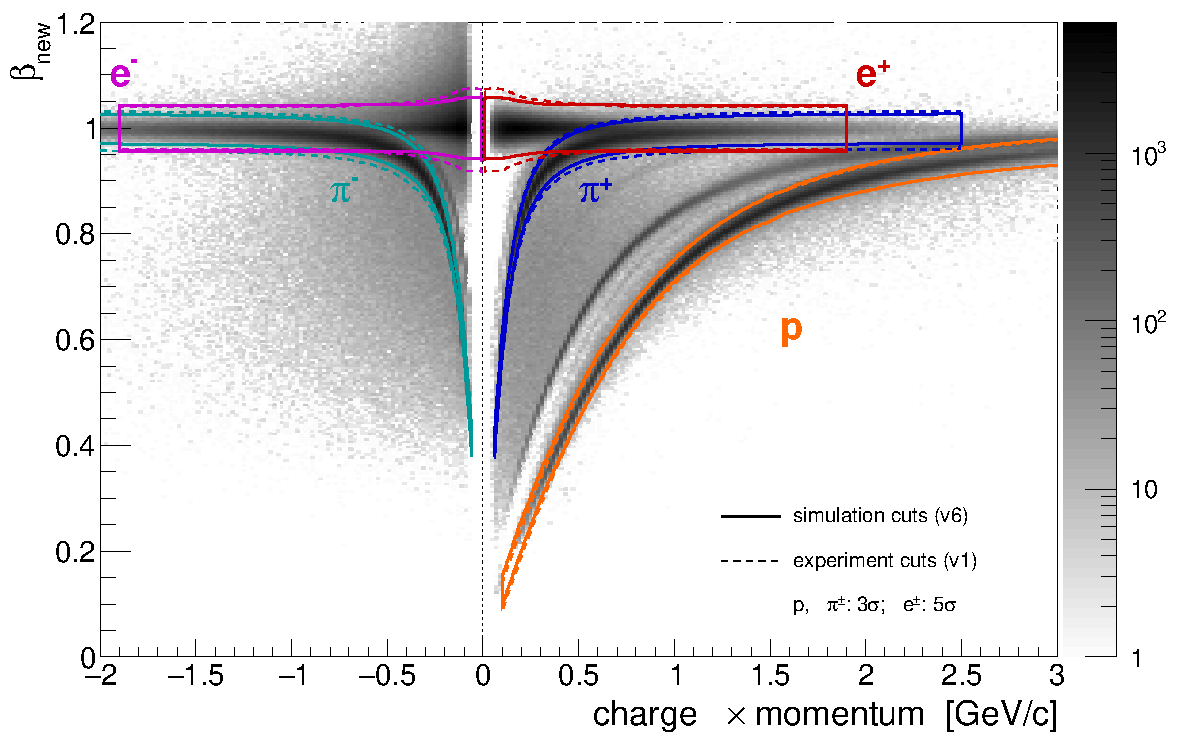
\includegraphics[width=\textwidth]{figs/banana_all.pdf}
\caption{$\betanew$ versus charge times momentum for simulated tracks before the PID cut
(SMASH p+p at 4.5\,GeV, no trigger condition, $\mathrm{isBest}=1$, vertex $z>-500$\,mm).
Protons and pions: hadron PID sample, slots of the hypothesis p\pip\pim (\code{HH_elossfix},
150 of 1000 files); $e^\pm$: lepton PID sample, lepton slots of the hypothesis \ppee
(\code{LEP_merged}, 101 files). Solid lines: simulation cuts (v6), dashed: experiment cuts
(v1); p and $\pi^\pm$ at $3\sigma$, $e^\pm$ at $5\sigma$. The weak band between the \pip and the
proton bands is made of protons in the \pip slot and of \pip in the proton slot
(see the text).}
\label{fig:banana}
\end{figure}

\begin{figure}[H]
\centering
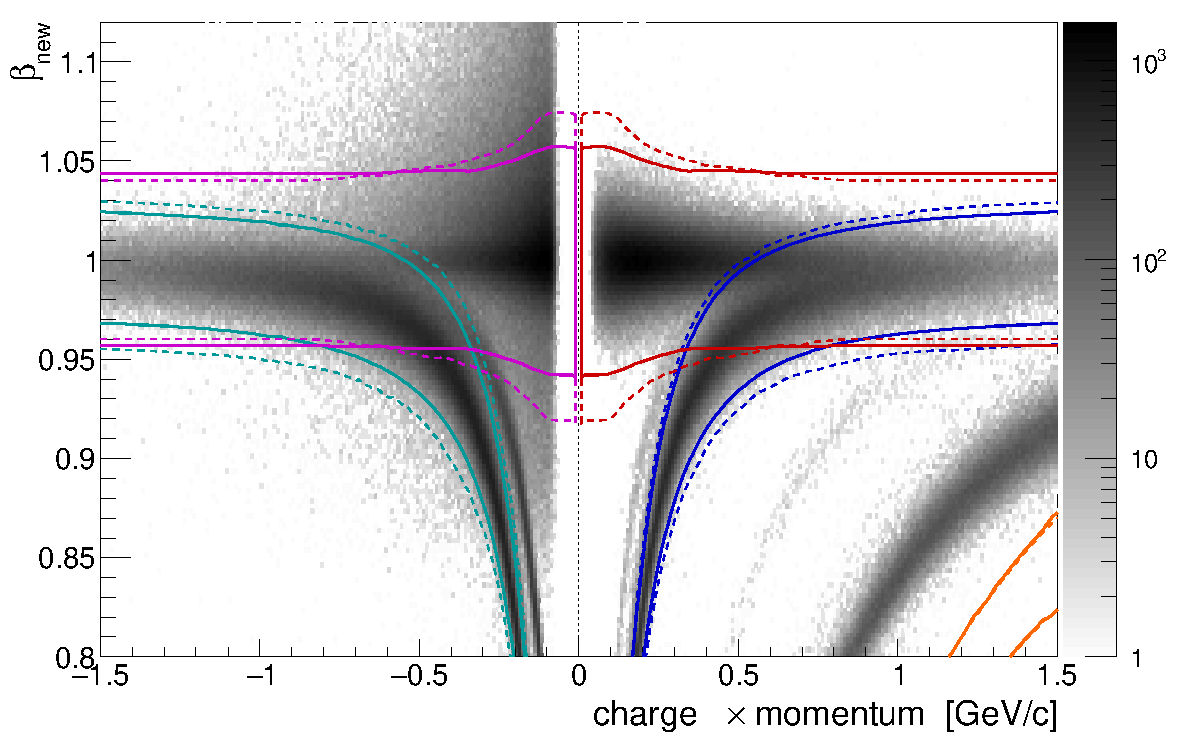
\includegraphics[width=\textwidth]{figs/banana_leptons.pdf}
\caption{The lepton region of the \ppee hypothesis before the PID cut (all four slots,
lepton PID sample). Above about 0.4\,\GeVc the pion bands enter the $e^\pm$ polygons: there
leptons are separated from pions by the RICH ring, not by $\betanew$. Lines as in
Fig.~\ref{fig:banana}.}
\label{fig:leptons}
\end{figure}

\textbf{Electrons without a RICH ring in the \pim slot.} In Fig.~\ref{fig:leptons} a second band runs
to the right of the \pim band, almost parallel to the \pim cut. It is made of electrons in the \pim
slot (Fig.~\ref{fig:pimslot}). A lepton slot takes only tracks with a correlated RICH ring
(Sect.~\ref{sec:ana}); an electron without one is treated as a hadron and can occupy the \pim slot.
Measured with the pion mass, it follows Eq.~(\ref{eq:half}) derived below, $1/\betanew = \tfrac12(1/\beta_e + 1/\beta_\pi)$.
The most probable $\betanew$ of these electrons is 0.76, 0.90 and 0.97 at $p = 0.1$, 0.2 and
0.4\,\GeVc (expected 0.74, 0.90, 0.97), while the \pim band lies at 0.61, 0.82 and 0.94. Muons
in the \pim slot (5\,\%) are shifted much less (0.846 against 0.821 at 0.2\,\GeVc) and lie mostly inside the
\pim cut.

These electrons are not a small effect: before the PID cut they are 16\,\% of the \pim slot (72\,769 of
456\,971 tracks), and the \pim cut keeps 23\,\% of them. This agrees with the 4.3\,\% of the rows of the
lepton-set \code{_ID} tree that have an electron in the \pim slot (bit 5 of \code{sim_flags}).
Table~\ref{tab:norich} compares them with the electrons that have a ring.

\begin{figure}[H]
\centering
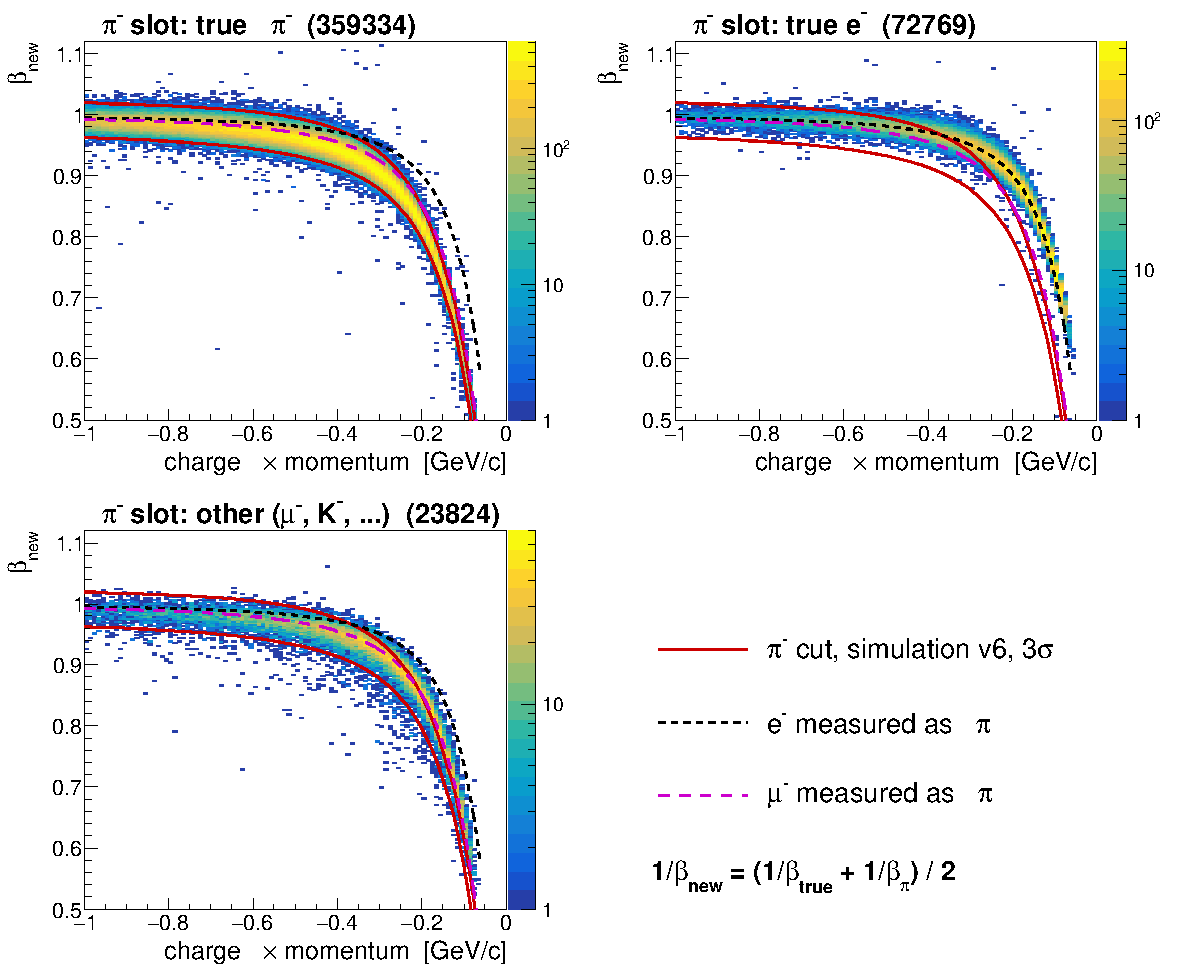
\includegraphics[width=0.92\textwidth]{figs/banana_pimslot.pdf}
\caption{The \pim slot of the \ppee hypothesis before the PID cut (lepton PID sample,
$\mathrm{isBest}=1$, vertex $z>-500$\,mm), split by the true particle: \pim, $e^-$, and the rest
(mostly $\mu^-$). Red: \pim cut (simulation v6, $3\sigma$). Dashed: $\betanew$ expected for an electron
(black) and a muon (magenta) measured with the pion mass, Eq.~(\ref{eq:half}).}
\label{fig:pimslot}
\end{figure}

\begin{table}[H]
\centering
\caption{Electrons without a RICH ring (in the \pim slot) and electrons with a ring (in the $e^-$
slot): GEANT creation process, parent particle and creation place, in percent of each group.
Lepton PID sample without PID cut, hypothesis \ppee, $\mathrm{isBest}=1$, vertex $z>-500$\,mm,
25 of the 101 files (18\,011 and 113\,135 electrons). Target region: $-200<z<-60$\,mm and $r<20$\,mm.
Macros \code{macros/norich.C}, \code{macros/norich_zr.C}; numbers in \code{tables/norich.txt}.}
\label{tab:norich}
\small
\begin{tabular}{@{}l r r@{}}
\toprule
 & $e^-$ in the \pim slot & $e^-$ in the $e^-$ slot \\
 & (no ring) & (ring) \\
\midrule
photon conversion ($\gamma\to\ee$)   & 86.6 & 35.2 \\
Compton scattering                    &  9.3 &  0.3 \\
knock-on (delta) electron             &  1.8 &  0.2 \\
decay (Dalitz decays of \piz, $\eta$) &  2.3 & 64.4 \\
\midrule
parent: photon / \piz / $\eta$        & 96.0 / 1.6 / 0.7 & 35.4 / 46.5 / 17.9 \\
\midrule
created in the target region          &  4.1 & 91.5 \\
created at $z = 200$--500\,mm          & 73.9 &  0.1 \\
created off the beam axis ($r>20$\,mm) & 95.8 &  7.7 \\
\midrule
ring found (\code{isring}) / lepton flag (\code{kIsLepton}) & 8.7 / 4.2 & 100 / 99.6 \\
ghost track (\code{sim_isghost})       & 29.2 & 8.9 \\
polar angle $\theta<18^\circ$          & 19.0 & 3.8 \\
\bottomrule
\end{tabular}
\end{table}

The electrons without a ring are secondary electrons of photons (mostly from \piz decays) produced
in the detector material \emph{downstream of the RICH radiator}:
\begin{itemize}
\item 28\,\% of their creation points lie within $\pm6$\,mm of a sphere of radius 872\,mm centred at
      $z\approx-625$\,mm. This is the RICH mirror: in the HGeant geometry (\code{rich.geo}) its radius is
      871--873\,mm and its centre is at $z = -532.2 - 88.5 = -620.7$\,mm. These are conversions in the
      mirror itself (carbon and glass segments).
\item Most of the others are created at $z\approx350$--500\,mm and $r\approx150$--350\,mm, about 0.6\,m
      from the target, which is the region of the first drift chambers (MDC~I). This attribution is
      inferred from the position; the HGeant medium numbers were not translated into material names.
\end{itemize}
They do not cross the \chem{C_4F_{10}} radiator, so they emit no Cherenkov light there: the missing
ring is expected and is not an inefficiency of the RICH. They still leave inner MDC segments and are
reconstructed as tracks.

\textbf{Charge asymmetry.} Ring-less positrons are rare: 0.6\,\% of the \pip slot against 16\,\% of
electrons in the \pim slot. This is not an effect of the hypothesis topology. In the hadron PID
sample without PID cut (hypothesis \pip\pim, \emph{all} combinations of 542\,211 events, every
distinct ring-less track counted once per event) the tracks created outside the target region give
$e^+ : e^- = 2\,633 : 24\,751$, a ratio of 0.106 (Table~\ref{tab:asym}). The ratio depends little on
the momentum but strongly on the polar angle. Of the conversion pairs, the positron partner of a
reconstructed electron is found in only 4.4\,\% of the cases, the electron partner of a reconstructed
positron in 38\,\%; both charges have the same ghost fraction (30--32\,\%), so the pair is not merged
into one track: the positron is lost. This agrees with the acceptance in the toroidal field: positive
particles are bent towards small polar angles and leave the acceptance, negative ones are bent
outwards. The strong dependence on $\theta$ supports this; the asymmetry that remains at large
$\theta$ and high momentum is not yet fully understood.

\begin{table}[H]
\centering
\caption{Ring-less $e^+$ (in the \pip slot) and $e^-$ (in the \pim slot) created outside the target
region, hadron PID sample without PID cut (\code{HH_elossfix}, 60 files, all combinations, each
track counted once per event; macro \code{macros/asym.C}).}
\label{tab:asym}
\small
\begin{tabular}{@{}l r r r@{\qquad}l r r r@{}}
\toprule
true $p$ [\MeVc] & $e^+$ & $e^-$ & $e^+/e^-$ & $\theta$ [deg] & $e^+$ & $e^-$ & $e^+/e^-$ \\
\midrule
0--100    & 302 & 1\,843 & 0.164 & $<20$  & 157 & 6\,814 & 0.023 \\
100--200  & 750 & 8\,403 & 0.089 & 20--30 & 585 & 6\,654 & 0.088 \\
200--300  & 564 & 5\,086 & 0.111 & 30--50 & 1\,125 & 7\,974 & 0.141 \\
300--500  & 551 & 5\,202 & 0.106 & 50--90 & 766 & 3\,309 & 0.231 \\
$>500$    & 466 & 4\,217 & 0.111 & & & & \\
\midrule
all       & 2\,633 & 24\,751 & 0.106 & & & & \\
\bottomrule
\end{tabular}
\end{table}

\textbf{Which cuts remove them.} After the PID cut, in the analysis ntuple of the standard set
(rules v2, base selection, $z>-160$\,mm), electrons are 2.5\,\% of the \pim slot (5\,464 rows); almost
all have $p>300$\,\MeVc, where the $\betanew$ bands of electrons and pions overlap, 95\,\% are
created at $z>100$\,mm and 90\,\% are conversions. Table~\ref{tab:eminpim} gives the fraction of
pions and electrons kept by candidate cuts.
\begin{itemize}
\item \textbf{Vertex cuts do not help:} a conversion electron continues in the direction of its
      photon, which came from the target, so its track points back to the vertex. The use in the
      vertex fit, the distance $|z_{\mathrm{trk}}-z_{\mathrm{vtx}}|$ and the distance $r$ from the beam
      axis keep electrons as often as pions.
\item \textbf{The energy loss in the MDC separates them:} median 2.75 for these electrons against 1.56
      for pions. A cut at 2.2 keeps 91.5\,\% of the pions and 15\,\% of the electrons, and lowers the
      electron share of the \pim slot from 2.5 to 0.4\,\%. Below 300\,\MeVc it keeps only 79\,\% of the
      pions (their energy loss rises), so a momentum-dependent cut is preferable.
\item Track $\chi^2$ and the angle to the nearest other track remove only about a quarter of them.
\end{itemize}
\emph{Not yet checked:} whether the MDC energy loss of simulation agrees with data, and whether the
high energy loss of these electrons is the relativistic rise or the double deposit of a close pair.

\begin{table}[H]
\centering
\caption{Fraction of true \pim and of electrons in the \pim slot kept by candidate cuts, analysis
ntuple \code{scan_nt} of the standard set (rules v2, after the PID cut, $z>-160$\,mm; macro
\code{macros/eminpim_cuts.C}; the lepton set gives the same picture). Numbers in
\code{tables/eminpim.txt}.}
\label{tab:eminpim}
\small
\begin{tabular}{@{}l c c c c@{}}
\toprule
 & \multicolumn{4}{c}{kept: \pim\ /\ $e^-$} \\
Cut & $p<300$\,\MeVc & 300--600\,\MeVc & $\ge600$\,\MeVc & all \\
\midrule
rows (\pim\ /\ $e^-$) & 54\,891 / 67 & 85\,475 / 3\,508 & 74\,669 / 1\,889 & 215\,035 / 5\,464 \\
\midrule
track used in the vertex fit & & & & 0.932 / 0.947 \\
$|z_{\mathrm{trk}}-z_{\mathrm{vtx}}|<20$\,mm & & & & 0.860 / 0.834 \\
$r<10$\,mm & & & & 0.938 / 0.949 \\
MDC $dE/dx<2.2$ & 0.787 / 0.373 & 0.965 / 0.165 & 0.951 / 0.105 & 0.915 / 0.147 \\
MDC $dE/dx<2.0$ & 0.679 / 0.239 & 0.921 / 0.058 & 0.891 / 0.035 & 0.849 / 0.053 \\
track $\chi^2<50$ & 0.886 / 0.851 & 0.920 / 0.769 & 0.949 / 0.790 & 0.921 / 0.777 \\
no track within 2$^\circ$ & 0.939 / 0.716 & 0.949 / 0.743 & 0.962 / 0.739 & 0.951 / 0.742 \\
\bottomrule
\end{tabular}
\end{table}

\textbf{$\betanew$ depends on the mass hypothesis of the track.} The relative-time method
(\code{HTimeCut}) takes one track $r$ of the combination as the time reference: an $e^-$ if
there is one, otherwise a proton, and among several candidates the one with the smallest
$\chi^2$. For every other track $j$ it uses the time
\begin{equation}
t_j^{\mathrm{new}} = t_j - \tfrac12\Big[\big(t_r - t_r^{\mathrm{exp}}\big) + \big(t_j - t_j^{\mathrm{exp}}\big)\Big],
\qquad \betanew = \frac{L_j}{c\,t_j^{\mathrm{new}}},
\label{eq:tnew}
\end{equation}
where $t$ is the measured time of flight, $t^{\mathrm{exp}} = L/(c\,\beta(p,m))$ the time
expected for the mass $m$ assumed in the hypothesis, and $L$ the path length. The start-time
correction is thus the average of the offsets $t - t^{\mathrm{exp}}$ of the reference and of
the track itself. For a track of the assumed mass the method gives its true velocity. For a
track of another mass half of the difference is absorbed; if the reference is correct,
\begin{equation}
\frac{1}{\betanew} = \frac12\left(\frac{1}{\beta_{\mathrm{true}}} + \frac{1}{\beta_{\mathrm{hyp}}}\right).
\label{eq:half}
\end{equation}
A proton of 1\,\GeVc in a \pip slot has $\betanew = 0.84$ instead of 0.73. A \pip in a proton
slot lands on the same curve, which is the weak middle band of Fig.~\ref{fig:banana}. The
reference track itself gets
$t_r^{\mathrm{new}} = t_r - \tfrac12(t_r - t_r^{\mathrm{exp}}) - \tfrac12\langle t_j - t_j^{\mathrm{exp}}\rangle_{j\neq r}$:
half of its own offset and half of the mean offset of its partners, so a wrongly assigned
partner shifts the velocity of the reference.

Figure~\ref{fig:hyp} shows what the PID cut acts on in this analysis: all four slots of the
\ppee hypothesis. The protons, which can only occupy the \pip and $e^+$ slots, form the band
of Eq.~(\ref{eq:half}) between the pion and the proton bands; only 7\,\% of them lie inside
the proton cut, and 2.6\,\% inside the \pip cut. Figure~\ref{fig:species} splits these tracks by
their true identity, and Table~\ref{tab:inside} gives the composition of each slot before the
PID cut together with the fraction of each kind of track inside the cut of the slot.

\begin{figure}[H]
\centering
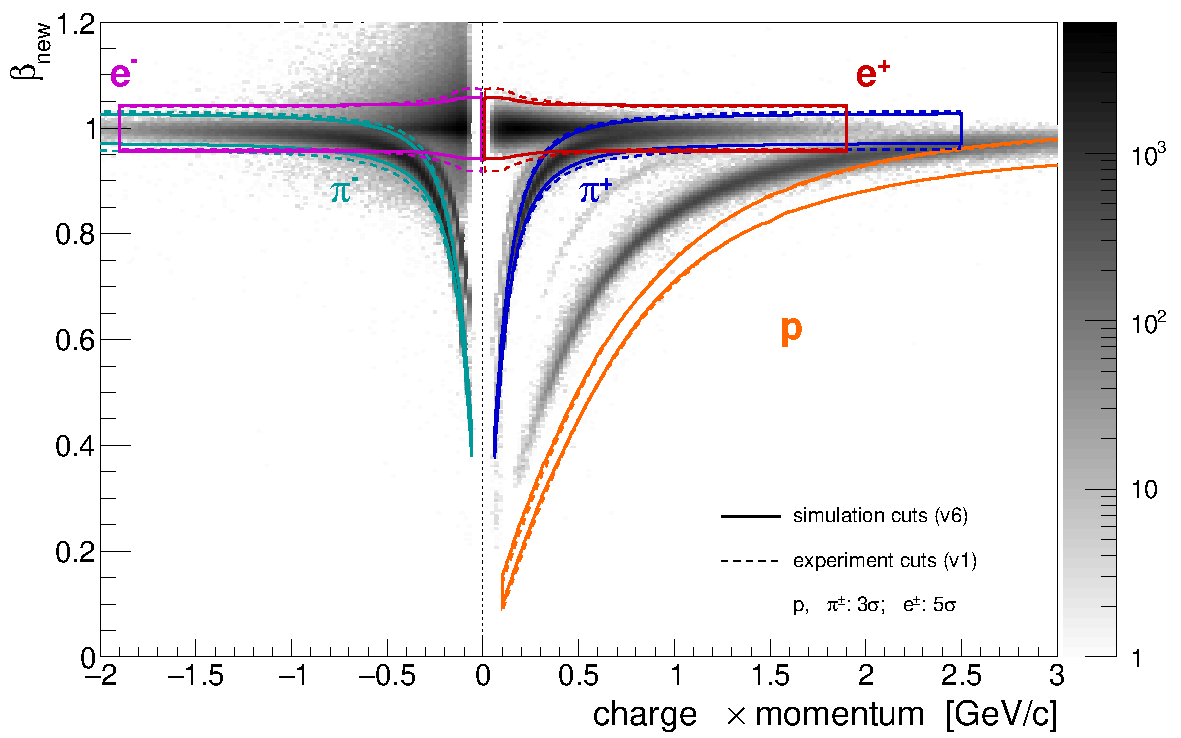
\includegraphics[width=\textwidth]{figs/banana_ppee.pdf}
\caption{All four slots of the \ppee hypothesis before the PID cut (lepton PID sample,
$\mathrm{isBest}=1$, vertex $z>-500$\,mm). The protons appear in the \pip and $e^+$ slots,
measured with the pion or electron mass, halfway between the pion and the proton bands.
Lines as in Fig.~\ref{fig:banana}.}
\label{fig:hyp}
\end{figure}

\begin{figure}[H]
\centering
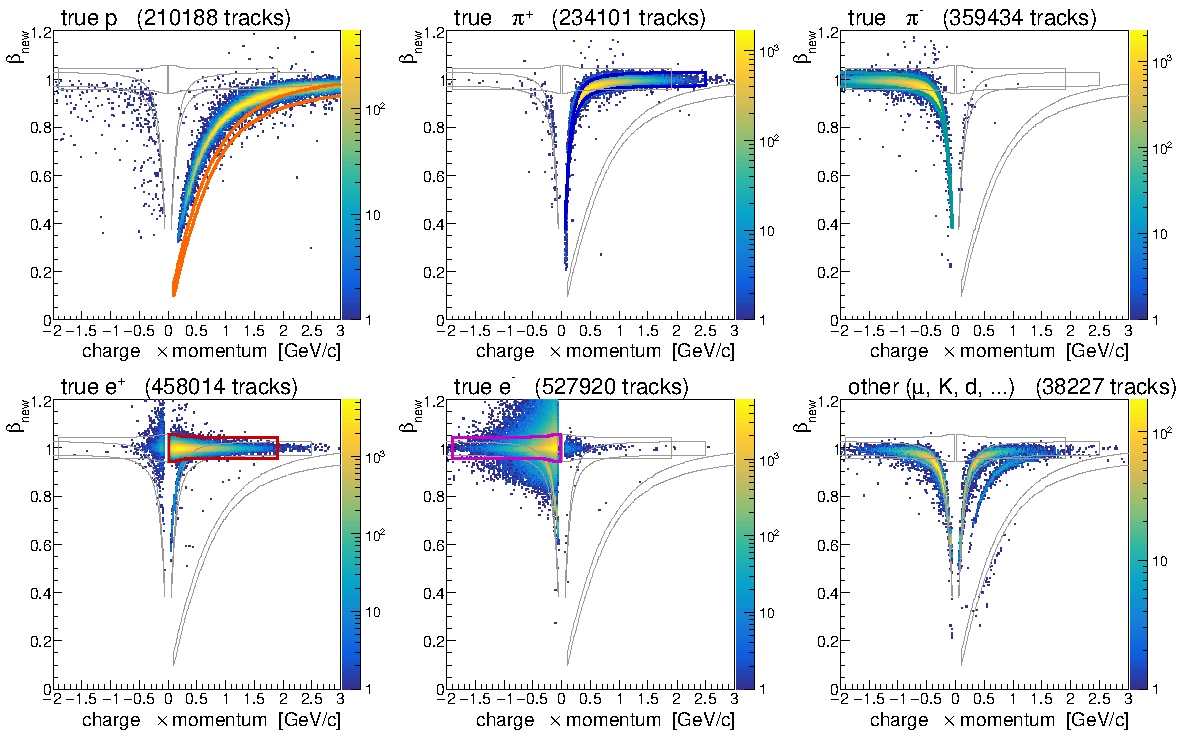
\includegraphics[width=\textwidth]{figs/banana_species.pdf}
\caption{The tracks of Fig.~\ref{fig:hyp} split by their true identity (GEANT). The coloured
polygon is the simulation cut of that species, the grey ones the other cuts.}
\label{fig:species}
\end{figure}

% generated by macros/rep_banana.C
\begin{table}[H]
\centering
\caption{Composition of the slots before the PID cut and the fraction of each kind of track that lies inside the simulation cut of its slot (v6; p, $\pi^\pm$ $3\sigma$, $e^\pm$ $5\sigma$). Each cell: share of the slot's tracks / fraction inside the cut. Simulation PID samples, $\mathrm{isBest}=1$, vertex $z>-500$\,mm, no trigger condition. Shares below 0.1\,\% are omitted.}
\label{tab:inside}
\footnotesize
\setlength{\tabcolsep}{4pt}
\begin{tabular}{@{}l r l l l l l l@{}}
\toprule
Hypothesis: slot & tracks & p & $\pi^+$ & $\pi^-$ & $e^+$ & $e^-$ & other \\
\midrule
p$\pi^+\pi^-$: p & 642804 & 0.889\,/\,0.936 & 0.104\,/\,0.010 & -- & -- & -- & 0.007\,/\,0.019 \\
p$\pi^+\pi^-$: $\pi^+$ & 642804 & 0.164\,/\,0.065 & 0.781\,/\,0.837 & -- & 0.005\,/\,0.228 & -- & 0.049\,/\,0.567 \\
p$\pi^+\pi^-$: $\pi^-$ & 642804 & -- & -- & 0.916\,/\,0.848 & -- & 0.032\,/\,0.254 & 0.051\,/\,0.636 \\
\midrule
$\pi^+\pi^-e^+e^-$: $\pi^+$ & 456971 & 0.453\,/\,0.026 & 0.510\,/\,0.988 & -- & 0.006\,/\,0.345 & -- & 0.031\,/\,0.682 \\
$\pi^+\pi^-e^+e^-$: $e^+$ & 456971 & 0.005\,/\,0.013 & 0.002\,/\,0.742 & -- & 0.991\,/\,0.999 & 0.002\,/\,0.989 & -- \\
$\pi^+\pi^-e^+e^-$: $\pi^-$ & 456971 & 0.002\,/\,0.313 & -- & 0.786\,/\,0.985 & -- & 0.159\,/\,0.228 & 0.052\,/\,0.668 \\
$\pi^+\pi^-e^+e^-$: $e^-$ & 456971 & -- & -- & -- & 0.005\,/\,0.840 & 0.994\,/\,0.837 & -- \\
\bottomrule
\end{tabular}
\end{table}


What the table shows:
\begin{itemize}
\item In the \ppee hypothesis the reference is the $e^-$, and the $e^-$ slot is 99.4\,\%
      pure. Correctly assigned pions and positrons then lie inside their cuts at the level
      expected from the cut widths: 98.8\,\% (\pip), 98.5\,\% (\pim), 99.9\,\% ($e^+$).
\item The $e^-$ itself, being the reference, is inside its cut only at 83.7\,\%: before the PID
      cut 45\,\% of the \pip slots hold a proton, and such a partner shifts the time of the
      reference. After the PID cut, when all partners must be inside their bands, this effect is
      much smaller.
\item In the p\pip\pim hypothesis there is no $e^-$, so the proton slot is the reference. With
      10\,\% \pip in the proton slot and 16\,\% protons in the \pip slot, even correctly assigned
      tracks lie inside their cuts at only 84--94\,\%.
\item Wrongly assigned tracks are mostly rejected: protons in a \pip slot pass the \pip cut at
      2.6\,\% (\ppee) and 6.5\,\% (p\pip\pim), \pip in a proton slot pass the proton cut at
      1.0\,\%.
\end{itemize}
The PID cut efficiency of a track therefore depends on its partners. Efficiencies have to be
taken from complete combinations, as the analysis does with the \code{_ID} trees and the GEANT
truth, and not from the width of single-track bands.

\subsection{Selection}
\label{sec:sel}
The base selection (``pre'') is common to all studies:
\begin{enumerate}
\item all combinations that passed the PID cuts, $\mathrm{isBest}\ge0$;
\item a reconstructed event vertex, $z>-500$\,mm (mandatory);
\item the PT3 trigger (data: \code{trigbit == 8192}; simulation: bit test);
\item the target region, $z>-160$\,mm (the target spans $-152$ to $-98$\,mm at half
      maximum, the maximum is at $-131$\,mm);
\item momenta corrected for the energy loss for all four particles (in data the corrected
      \pim momentum is missing for 0.7\,\% of the rows, \pim at $\theta<16^\circ$; such rows are
      dropped).
\end{enumerate}
On top of it the analysis studies the cuts of Table~\ref{tab:cuts}. Each of them is stored in
\code{scan_nt} both as a value and as a pass flag, so that every cut can be scanned and its
effect shown separately.

\begin{table}[H]
\centering
\caption{Cut variables of the analysis. All are computed from the corrected momenta.
The values are those of the named selections used so far; the cut scan of the data is
summarised in a later part.}
\label{tab:cuts}
\begin{tabularx}{\textwidth}{@{}l L l@{}}
\toprule
Variable & Meaning & Values used \\
\midrule
OA & opening angle of the \ee pair (lab) & $>2^\circ$ (conversions) \\
$\alpha_{\mathrm{lab}}$ & angle between the \pipi and the \ee systems (lab) & $<50^\circ$, 55, 40 \\
\Mpipi & invariant mass of the pions & $<0.42$, $<0.46$, $>0.30$\,\GeVcc \\
$\alpha_\eta$ & angle between \pipi and \ee in the rest frame of a hypothetical $\eta$ with the measured \ppee momentum and the mass $m_\eta$ (a band-pass in \Mfour) & $>140^\circ$ \\
pions in vertex & both pions used in the event-vertex fit (\code{isUsedVertex}) & flag \\
$\Delta z_\pi$ & $\max(|z_{\pi^+}-z_{\mathrm{vertex}}|, |z_{\pi^-}-z_{\mathrm{vertex}}|)$, $z$ of a track at its closest approach to the beam axis & $<40$\,mm \\
$\mathrm{MM}_4$, $p_{T,4}$ & missing mass of \ppee, the mass of (beam + target $-$ \ppee) four-momenta; transverse momentum of \ppee (lab) & studied \\
\bottomrule
\end{tabularx}
\end{table}

\begin{table}[H]
\centering
\caption{Named selections (all include ``pre'').}
\label{tab:presets}
\begin{tabular}{@{}l l@{}}
\toprule
Name & Cuts in addition to ``pre'' \\
\midrule
pre+OA$>2$ & OA $>2^\circ$ \\
slides & $\alpha_{\mathrm{lab}}<50^\circ$, $\Mpipi<0.46$\,\GeVcc, $\alpha_\eta>140^\circ$, OA$>2^\circ$ \\
old code & $\alpha_{\mathrm{lab}}<50^\circ$, $\Mpipi<0.42$\,\GeVcc, $\alpha_\eta>140^\circ$ \\
peak nominal & $\alpha_{\mathrm{lab}}<55^\circ$, $\Mpipi>0.30$\,\GeVcc \\
bump nominal & $\alpha_{\mathrm{lab}}<40^\circ$, $0.30<\Mpipi<0.41$\,\GeVcc \\
\bottomrule
\end{tabular}
\end{table}

\subsection{Software chain}
\begin{enumerate}
\item \textbf{PAT}, PostDST Analysis Tool (\code{git.gsi.de/przygoda/pat3}): DST $\to$ hypothesis ntuples with PID,
      relative-time reconstruction and ranking; simulation branch \code{pp45_sim_pippimepem}.
\item \textbf{FAT}, Final Analysis Tool (this repository, branch \code{pp45_pippimepem_betanew_sim}): base
      selection, kinematics, truth classes and weights (\code{src/sim_truth.h}), ntuple
      \code{scan_nt}; configurations \texttt{config\_sim\_\{std,lep,eta\}*.json}.
\item \textbf{Macros} (\code{plots/eta_sim/}): the common engine \code{SimEngine.h} (compact
      files, components, presets, weighted spectra with event-grouped errors) and the studies;
      figures in \code{plots/eta_sim/figs/}, tables in \code{plots/eta_sim/tables/}.
\end{enumerate}

% sec5_sim.tex -- Section "Simulation study: from the signal to the selection" of report.tex
% (to be \input in place of the planned section 5). Simulation only. Macros: plots/eta_sim/s5_*.C,
% tables: plots/eta_sim/tables/s5_*.txt, figures: plots/eta_sim/figs/s5_*.pdf (copied to figs/).
%======================================================================
\section{Simulation study: from the signal to the selection}
\label{sec:simres}
%======================================================================
This section follows the order planned for the study (signal, acceptance, cuts, backgrounds,
optimisation, test of the extraction). It uses \textbf{simulation only}: no measured data were
read. The simulation contains no combinatorial background (CB), and none was added. All
statements about cuts therefore concern the physical background of SMASH, not the CB of the data.

\textbf{Common settings.} Every number of this section uses the same rows and weights:
\begin{itemize}
\item rows of the \ppee trees of the three sets (std, lep, $\eta$), owned in mode~A
      (Sect.~\ref{sec:weights});
\item the weight $W$ of Sect.~\ref{sec:weights} (PDG branching ratios) times the physics
      weights of the $\eta$ decays, main variant V3 (Sect.~\ref{sec:etagen}); for the bump the
      KLOE-2 Dalitz plot, for the conversion peak $|F_V|^2p^{*2}k^2$. All numbers of this section
      use the weight rules~v2 (exact HGeant branching ratios, Sect.~\ref{sec:hgeanteta});
\item the base selection ``pre'' (Sect.~\ref{sec:sel}); all cut variables from the corrected momenta;
\item cross section $\sigma = \sum W/\Lsim$ with $\Lsim = 221.05\,\nbinv$;
\item statistical errors from event groups: the variance of a sum is the sum over events of
      the squared sum of the weights of their rows. The effective number of rows,
      $N_{\mathrm{eff}} = (\sum W)^2/\mathrm{Var}$, is quoted where it is small;
\item where a number of rows in data is needed (significance, expected limits), the
      luminosity $\Ldata = 6080.5\,\nbinv$ (UNCONFIRMED) is used as a scale only: one unit of
      $\sum W$ corresponds to 27.51 expected rows.
\end{itemize}
The simulated sum is template T1 (signal classes 2--5) plus template T2 (physical background).
Templates T3 (fake lepton) and T4 (leptons from two sources) are never added; they are
shown separately and enter a background only as a stated variant. X17 rows (class~6) carry
$W = 2\,\mathrm{BR}$ per row, BR is a free parameter, and they are never added to the sum.
The windows in \Mfour and the background groups are the same in all parts
(Table~\ref{tab:s5defs}).

\begin{table}[H]
\centering
\caption{Windows in \Mfour and background groups used in this section. The peak window is
centred on the simulated peak ($0.5460\pm1.9\times0.0067$\,\GeVcc); the bump window is the
data bump window scaled by the simulated mass scale 1.0057. The groups split template~2 by the
lepton-pair class (L) and the pion-pair class (P) of \code{src/sim_truth.h} (all classes and the
templates T1--T4 are defined in Table~\ref{tab:classes}); a row goes to the first group in the order
given whose condition it fulfils.}
\label{tab:s5defs}
\small
\begin{tabularx}{\textwidth}{@{}l L@{}}
\toprule
Name & Definition \\
\midrule
peak window  & $0.5333 \le \Mfour < 0.5587$\,\GeVcc \\
bump window  & $0.4576 \le \Mfour < 0.5255$\,\GeVcc \\
other regions & below 0.4576; gap 0.5255--0.5333; 0.5587--0.70; 0.70--1.00; above 1.00\,\GeVcc \\
\midrule
classes 2, 3, 4, 5 & the signal classes (Table~\ref{tab:cls}): bump Dalitz, bump conversion,
   peak conversion, direct decay \\
$G_\eta$   & template 2 with both pions from one $\eta$ (P2) or an $\eta$ Dalitz pair (L2):
   an $\eta$ is produced, but the row is not a signal combination \\
$G_{\pi^0\mathrm{D}}$ & remaining template-2 rows with a \piz Dalitz pair (L1) \\
$G_{\mathrm{conv}}$ & remaining template-2 rows with a conversion pair (L3) \\
$G_{\mathrm{vec}}$  & remaining template-2 rows with $\rho^0,\omega,\phi\to\ee$, $\omega\to\piz\ee$
   or a second-decay pair (L4--L6) \\
$G_{\mathrm{oth}}$  & all other template-2 rows (in practice the \ee pair of a direct
   $\eta\to\ppee$ decay with pions from elsewhere) \\
$G_{\mathrm{fake}}$, $G_{\mathrm{diff}}$ & template 3 and template 4 (variants only) \\
multi-pion & $G_{\pi^0\mathrm{D}} + G_{\mathrm{conv}} + G_{\mathrm{vec}}$ \\
\bottomrule
\end{tabularx}
\end{table}

%----------------------------------------------------------------------
\subsection{The full spectrum and the cut sequence}
\label{sec:s5spec}
%----------------------------------------------------------------------
\textbf{The spectrum after ``pre''} (Fig.~\ref{fig:s5full}). The simulated sum is
$\sigma(\mathrm{T1+T2}) = 701.1\pm1.5$\,nb over all \Mfour. Of this, the four signal classes
are $14.89\pm0.27$\,nb and the multi-pion background $659.9\pm1.4$\,nb (94\,\%):
$G_{\pi^0\mathrm{D}} = 394.5\pm0.8$\,nb, $G_{\mathrm{conv}} = 265.3\pm1.2$\,nb and
$G_{\mathrm{vec}} = 0.107\pm0.001$\,nb. $G_\eta$ is $24.27\pm0.21$\,nb and $G_{\mathrm{oth}}$
$1.967\pm0.005$\,nb. Not in the sum: T3 $125.0\pm0.7$\,nb, T4 $12.51\pm0.25$\,nb. Above the
kinematic limit $\Mfour = \sqrt{s}-2m_p = 1.591$\,\GeVcc there are 2.87\,nb (0.4\,\%); 2.58\,nb
of them contain a misidentified track.

\begin{figure}[H]
\centering
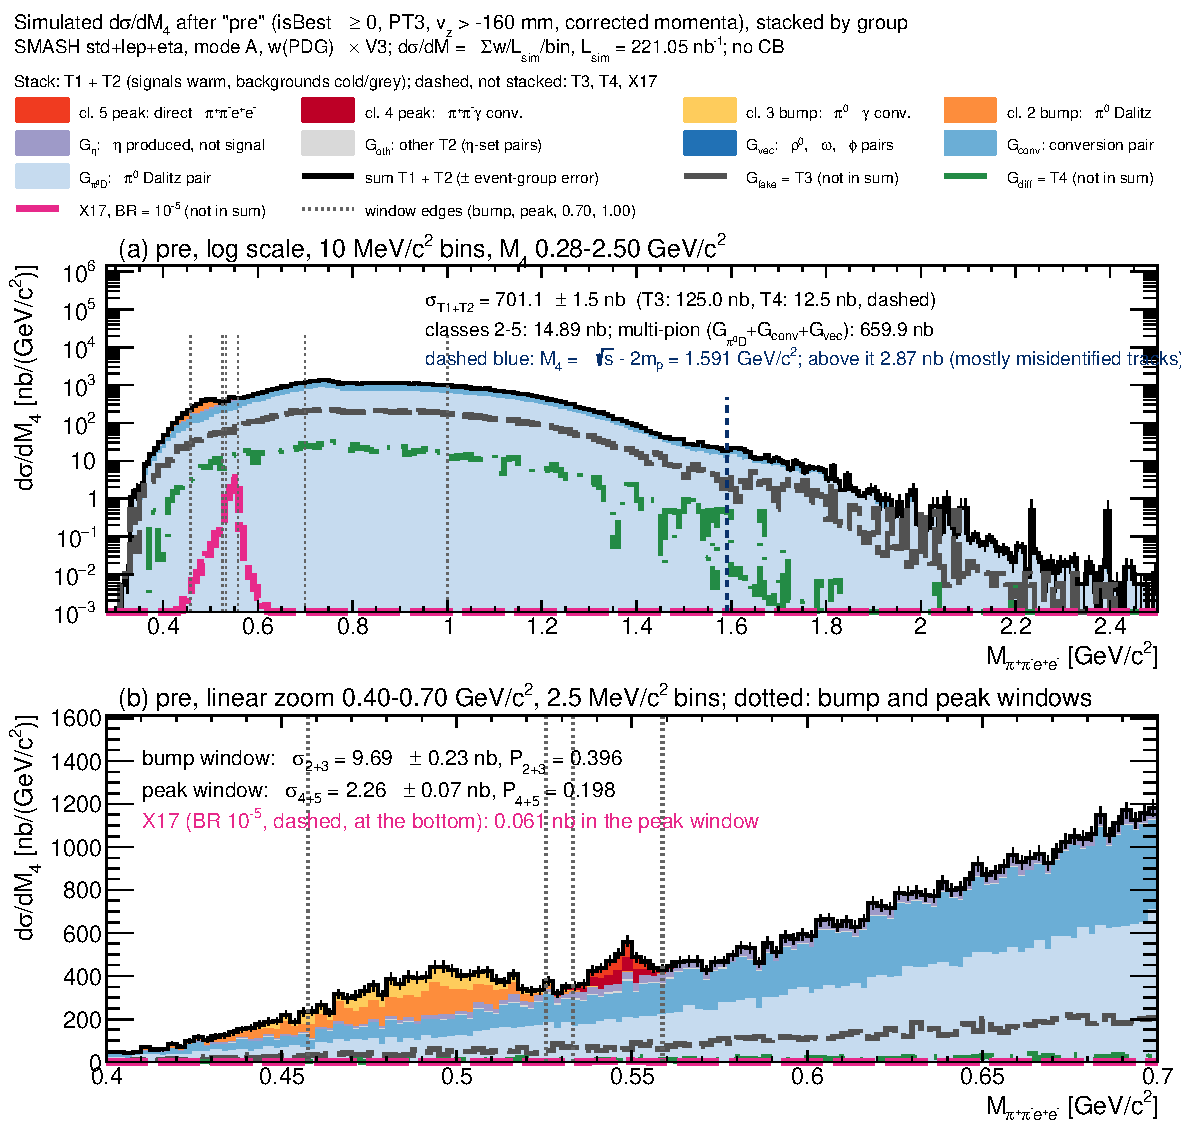
\includegraphics[width=\textwidth]{figs/s5_spec_full_pre.pdf}
\caption{Simulated $d\sigma/d\Mfour$ after ``pre'', stacked by group (signal classes warm,
background groups cold or grey). Dashed and not stacked: T3, T4 and X17 at
$\mathrm{BR} = 10^{-5}$. (a) Log scale, 10\,\MeVcc bins; the dashed blue line is the kinematic
limit. (b) Linear zoom, 2.5\,\MeVcc bins, with the bump and peak windows (dotted).}
\label{fig:s5full}
\end{figure}

\textbf{The cut sequence.} The four $\eta$-selection cuts of the analysis are applied one after
the other: $\mathrm{OA}>2^\circ$, $\alpha_{\mathrm{lab}}<50^\circ$, $\Mpipi<0.46$\,\GeVcc,
$\alpha_\eta>140^\circ$. All four together are the selection ``slides''.
Table~\ref{tab:s5flow} gives the cross sections, the purity $P$ = (signal in the window)/(T1+T2 in
the window) and $F = S/\sqrt{S+B}$, with $S$ the signal rows and $B$ the other T1+T2 rows of the
window at \Ldata. Figure~\ref{fig:s5steps} shows the spectrum after each step.

\begin{table}[H]
\centering
\caption{Cut sequence (nominal order). $\sigma$ in nb, errors from event groups. $P$: purity in
the window. $F = S/\sqrt{S+B}$ at $\Ldata = 6080.5\,\nbinv$ (UNCONFIRMED); in brackets $F$ with
$B$ + T3 + T4. Columns: the cuts OA$>2^\circ$, $\alpha_{\mathrm{lab}}<50^\circ$, $\Mpipi<0.46$\,\GeVcc and
$\alpha_\eta>140^\circ$ added one by one; last column: the final selection with $\Mpipi<0.42$\,\GeVcc.}
\label{tab:s5flow}
\footnotesize
\setlength{\tabcolsep}{3pt}
\begin{tabular}{@{}l rrrrr r@{}}
\toprule
 & pre & +OA & +$\alpha_{\mathrm{lab}}$ & +$M_{\pi\pi}$ & +$\alpha_\eta$ & $M_{\pi\pi}<0.42$ \\
\midrule
T1+T2, all $M_4$        & $701.1\pm1.5$ & $476.4\pm1.1$ & $254.0\pm0.9$ & $89.6\pm0.5$ & $67.9\pm0.5$ & $53.0\pm0.4$ \\
classes 2--5, all $M_4$ & $14.89\pm0.27$ & $10.58\pm0.22$ & $10.10\pm0.22$ & $10.06\pm0.22$ & $7.60\pm0.18$ & 7.26 \\
\midrule
bump: classes 2+3      & $9.69\pm0.23$ & $6.88\pm0.20$ & $6.61\pm0.19$ & $6.61\pm0.19$ & $5.60\pm0.17$ & $5.59\pm0.17$ \\
bump: T1+T2            & $24.48\pm0.33$ & $17.93\pm0.28$ & $16.71\pm0.27$ & $16.71\pm0.27$ & $15.08\pm0.25$ & $14.84\pm0.25$ \\
bump: $P$              & $0.396\pm0.007$ & $0.383\pm0.008$ & $0.395\pm0.008$ & $0.395\pm0.008$ & $0.371\pm0.008$ & $0.377\pm0.008$ \\
bump: $F$              & $152.7\pm3.0$ & $126.6\pm3.0$ & $126.0\pm3.0$ & $126.0\pm3.0$ & $112.5\pm2.9$ & $113.2\pm2.9$ \\
                       & (143.2) & (119.3) & (119.0) & (119.0) & (106.2) & (106.9) \\
\midrule
peak: classes 4+5      & $2.26\pm0.07$ & $1.57\pm0.05$ & $1.40\pm0.05$ & $1.37\pm0.05$ & $1.37\pm0.05$ & $1.07\pm0.04$ \\
peak: T1+T2            & $11.45\pm0.18$ & $8.45\pm0.15$ & $6.97\pm0.14$ & $6.79\pm0.13$ & $6.79\pm0.13$ & $5.64\pm0.12$ \\
peak: $P$              & $0.198\pm0.006$ & $0.185\pm0.006$ & $0.201\pm0.007$ & $0.202\pm0.007$ & $0.202\pm0.007$ & $0.190\pm0.007$ \\
peak: $F$              & $52.1\pm1.5$ & $42.0\pm1.3$ & $41.5\pm1.4$ & $41.0\pm1.4$ & $41.0\pm1.4$ & $35.3\pm1.2$ \\
                       & (48.1) & (39.0) & (38.4) & (38.0) & (38.0) & (32.6) \\
\bottomrule
\end{tabular}
\end{table}

\begin{figure}[H]
\centering
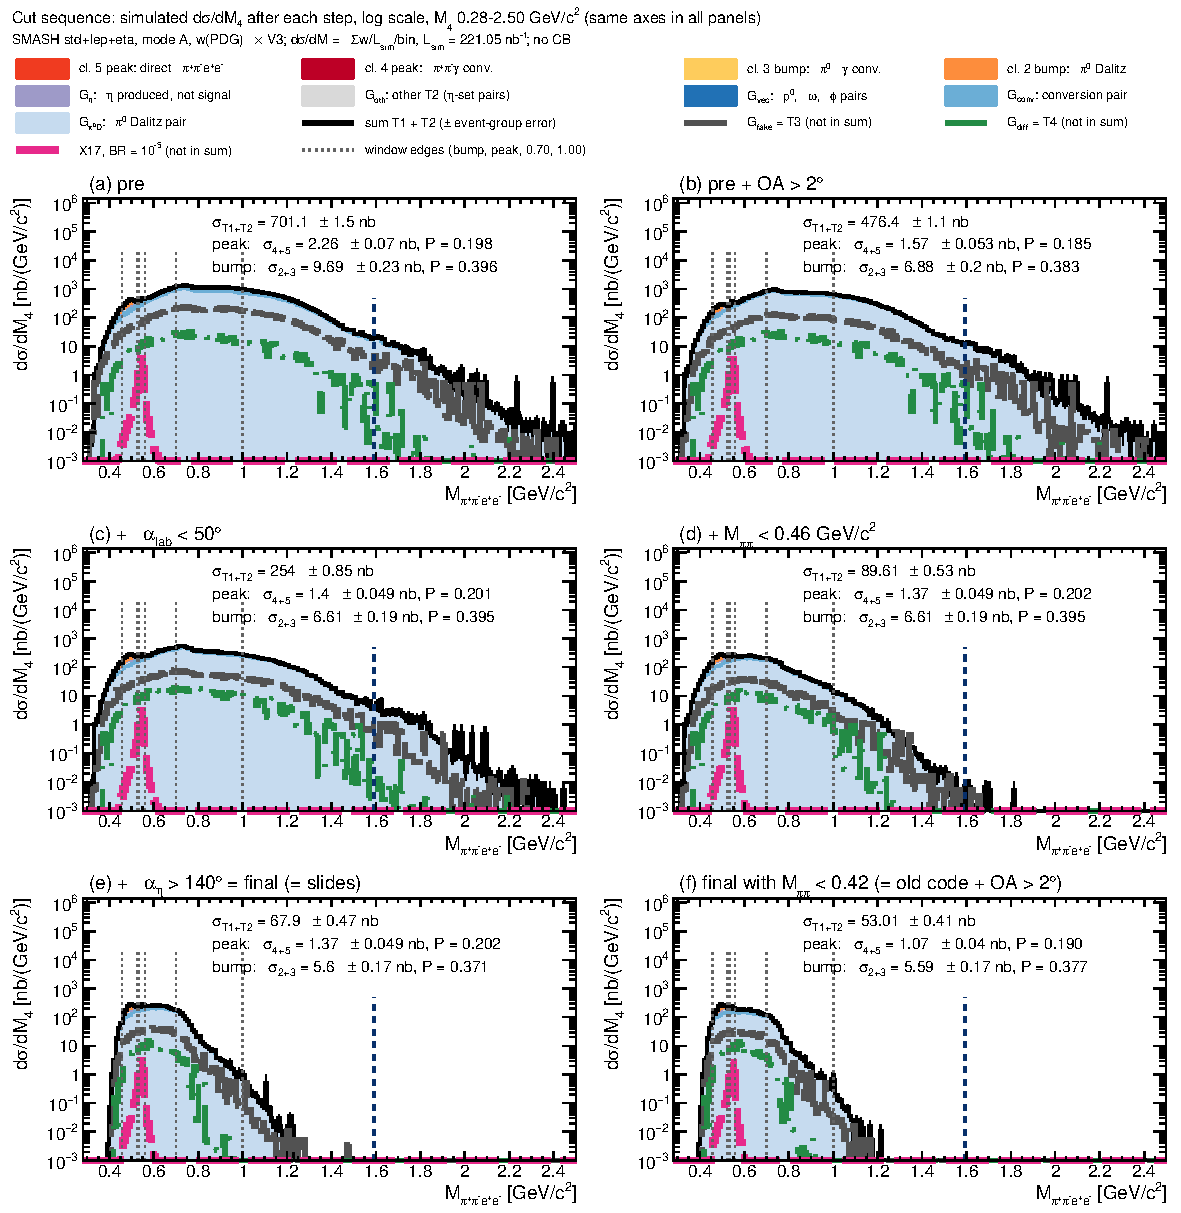
\includegraphics[width=\textwidth]{figs/s5_spec_steps_log.pdf}
\caption{Simulated $d\sigma/d\Mfour$ after each step of the cut sequence (same axes in all
panels; legend as in Fig.~\ref{fig:s5full}). (a) pre; (b)--(e) the four cuts added one by one;
(e) is ``slides''; (f) the final selection with $\Mpipi<0.42$\,\GeVcc.}
\label{fig:s5steps}
\end{figure}

\textbf{Where each cut acts.} Table~\ref{tab:s5where} gives, for each cut applied alone to
``pre'', the fraction of the background of each \Mfour region that it removes.
\begin{itemize}
\item OA$>2^\circ$ removes 25--36\,\% of the background in every region: it acts everywhere the same.
\item $\alpha_{\mathrm{lab}}$ and \Mpipi act mainly above the $\eta$: \Mpipi$<0.46$ removes
      nothing in the bump window, because there $\Mpipi\le\Mfour-\Mee$ is already below the
      limit, and 1.8\,\% in the peak window.
\item $\alpha_\eta$ is a band-pass in \Mfour. It is the angle between \pipi and \ee in a frame
      obtained by boosting with the measured total momentum and an energy computed with the
      $\eta$ mass (\code{Physics::}\allowbreak\code{openingAngleInMassConstrainedRestFrame}). For
      $\Mfour = m_\eta$ this frame is the true rest frame and the angle is exactly $180^\circ$. In
      the peak window the cut therefore removes nothing (efficiency 1.000 for every group); it
      removes 75\,\% of the background below the bump, 78\,\% in 0.70--1.00 and 99\,\% above
      1.00\,\GeVcc, and 10--14\,\% of the bump signal in the bump window.
\end{itemize}

\begin{table}[H]
\centering
\caption{Fraction of the background removed by each cut alone (from ``pre''). Background: T1+T2
minus the signal of the window in the bump and peak windows, T2 elsewhere. Errors 0.002--0.012
in the first three columns, below 0.002 elsewhere.}
\label{tab:s5where}
\footnotesize
\setlength{\tabcolsep}{4pt}
\begin{tabular}{@{}l rrrrrr r@{}}
\toprule
cut & $<0.4576$ & bump & peak & 0.56--0.70 & 0.70--1.00 & $>1.00$ & all \Mfour (T2) \\
\midrule
OA$>2^\circ$                     & 0.247 & 0.252 & 0.250 & 0.276 & 0.317 & 0.363 & 0.321 \\
$\alpha_{\mathrm{lab}}<50^\circ$ & 0.014 & 0.077 & 0.166 & 0.307 & 0.473 & 0.559 & 0.455 \\
$\Mpipi<0.46$\,\GeVcc            & 0.000 & 0.0005 & 0.018 & 0.254 & 0.631 & 0.876 & 0.616 \\
$\alpha_\eta>140^\circ$          & 0.751 & 0.053 & 0.000 & 0.075 & 0.781 & 0.987 & 0.702 \\
\bottomrule
\end{tabular}
\end{table}

\textbf{The order of the cuts matters for the attribution.} Inside the two windows the cuts
act almost independently: the fraction attributed to a cut changes by 10--20\,\% (relative)
between the nominal and the reverse order. Over the whole spectrum it changes completely:
$\alpha_\eta$ removes 69\,\% of T1+T2 when applied first, but 3\,\% when applied last. A
statement ``this cut removes that much background'' is therefore meaningful only per window and
together with the order.

\textbf{The resulting shape.} After ``slides'' the multi-pion background is still the largest
part of every window: 0.72 below the bump, 0.55 in the bump window, 0.70 in the peak window,
0.89 in 0.56--0.70\,\GeVcc. T1+T2 above 0.70\,\GeVcc drops from 545.9 to 9.96\,nb, from 78\,\% to
15\,\% of the spectrum. Above 1.00\,\GeVcc only 0.037\,nb remain, with $N_{\mathrm{eff}} = 33$.

\notebox{\textbf{Main result of the spectrum study.} In the simulation the four cuts do not
raise the purity of either window (bump $0.396\to0.371$, peak $0.198\to0.202$), and $F$ falls at
every step (peak $52.1\to41.0$, bump $152.7\to112.5$). What the cuts do is remove the multi-pion
background outside the windows. A gain from these cuts in data can only come from what the
simulation does not contain: the CB, or a data/SMASH difference of the multi-pion background.
This must be checked with data.}

%----------------------------------------------------------------------
\subsection{The signal at generator level}
\label{sec:s5gen}
%----------------------------------------------------------------------
\textbf{Number of produced decays.} The PLUTO generator file of the $\eta$ set holds the true
kinematics of $N = 1\,181\,801$ direct decays from 1000 of the 100\,000 files. Assuming these
files are representative, the set contains $N_{\mathrm{direct}} = 100\,N = 1.1818\times10^{8}$
direct decays. Every $\eta$ of the set is forced, half into the direct decay, so the set holds
$N_\eta = 2N_{\mathrm{direct}} = 2.364\times10^{8}$ $\eta$ mesons, i.e.
$\sigma(pp\to\eta X) = N_\eta/\Lsim = 1.069$\,mb in SMASH. The decays of the other channels
are $N_\eta$ times the PDG branching ratio (Table~\ref{tab:s5prod}). The statistical error of
this scale is 0.09\,\%; whether the 1000 files are representative is UNVERIFIED.

\begin{table}[H]
\centering
\caption{Produced decays per set ($10^{10}$ events) and production cross sections, from
$N_\eta$ and PDG branching ratios. Class 3 is counted per $\eta\to\pipi\piz$ decay with any \piz
decay (the conversion happens in the detector), class 4 per $\eta\to\pipi\gamma$ decay. Scale
error 0.09\,\% for every row.}
\label{tab:s5prod}
\small
\begin{tabular}{@{}l l r r@{}}
\toprule
Class & Channel & produced decays & $\sigma_{\mathrm{prod}}$ [nb] \\
\midrule
2 & $\eta\to\pipi\piz$, $\piz\to\ee\gamma$ & $6.360\times10^{5}$ & 2\,877.2 \\
3 & $\eta\to\pipi\piz$ (any \piz decay)     & $5.417\times10^{7}$ & 245\,075 \\
4 & $\eta\to\pipi\gamma$                    & $9.974\times10^{6}$ & 45\,123 \\
5 & $\eta\to\ppee$                          & $6.334\times10^{4}$ & 286.56 \\
6 & $\eta\to\pipi X17$, $X17\to\ee$, $\mathrm{BR}=10^{-5}$ & $2.364\times10^{3}$ & 10.693 \\
\bottomrule
\end{tabular}
\end{table}

\textbf{Shapes} (Fig.~\ref{fig:s5gen}). The physics weights replace the generator
distribution of the direct decay by Kroll--Wada $\times$ the P-wave rate $\times$ the form
factors $\times$ the decay angles (V3). The \Mee spectrum then becomes much harder:
\begin{center}
\small
\begin{tabular}{@{}l rrrrr@{}}
\toprule
fraction of produced decays with $\Mee >$ & 2 & 10 & 17 & 20 & 50\,\MeVcc \\
\midrule
direct, generator     & 0.513 & 0.099 & 0.057 & 0.047 & 0.016 \\
direct, V3            & 0.868 & 0.478 & 0.351 & 0.313 & 0.118 \\
bump \piz Dalitz (Kroll--Wada) & 0.860 & 0.443 & 0.308 & 0.268 & 0.070 \\
\bottomrule
\end{tabular}
\end{center}
The mean \Mpipi is 0.4007\,\GeVcc for the direct decay (V3), 0.3623 for the bump (KLOE-2; phase
space 0.3465), 0.4057 for the conversion peak ($|F_V|^2$; phase space 0.4014) and 0.3985 for X17
(three-body phase space, ASSUMED). The bump ends at $m_\eta-m_{\piz} = 0.413$\,\GeVcc.

\textbf{Direct decays under the X17 line.} The direct decay has a continuous \Mee spectrum and
contributes under any X17 line. With V3, the produced direct decays within $|\Mee-17| < d$ are
4.04, 7.95, 15.9 and 32.4\,nb for $d = 0.5$, 1, 2 and 4\,\MeVcc; X17 with
$\mathrm{BR}=10^{-5}$ is 10.69\,nb (Fig.~\ref{fig:s5gen}d).

\begin{figure}[H]
\centering
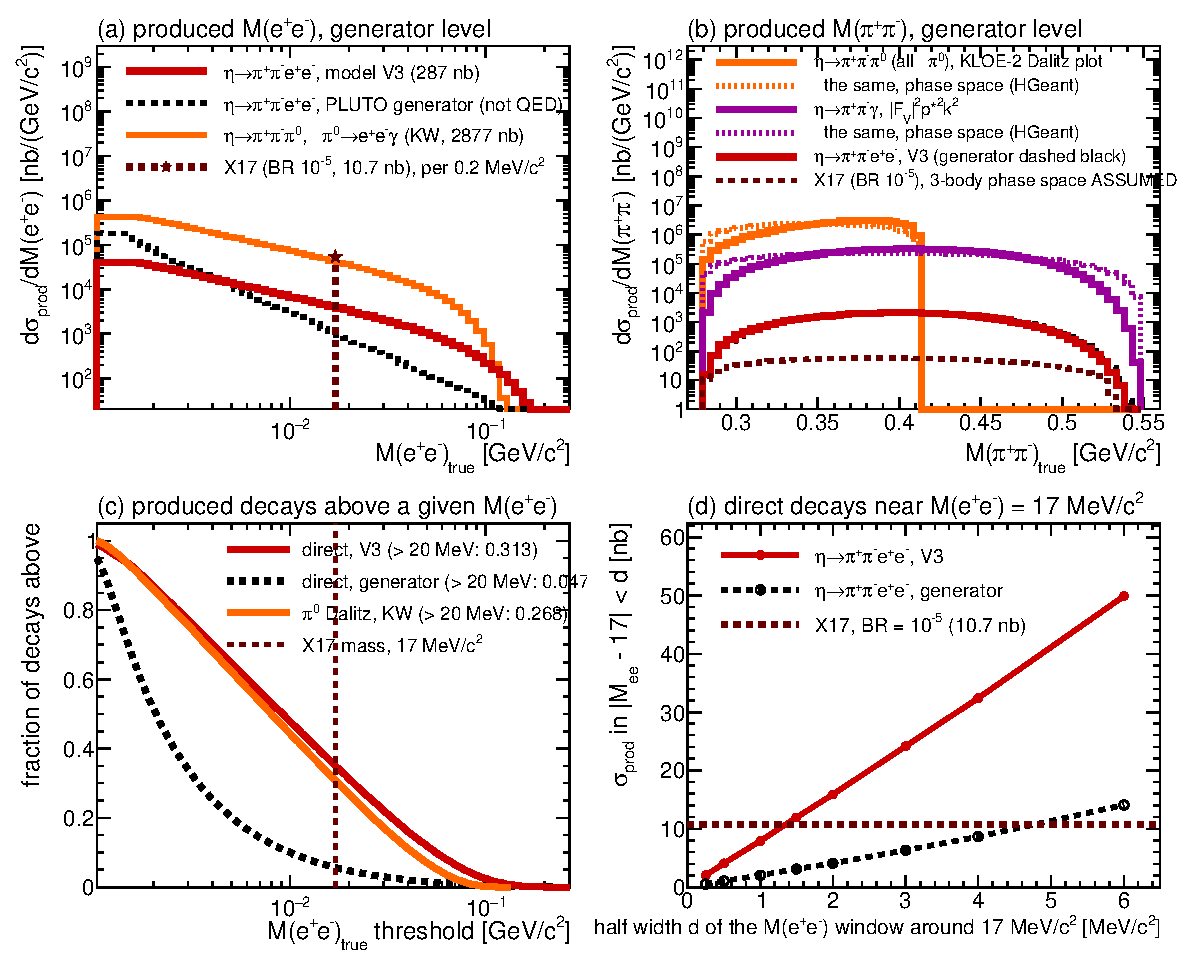
\includegraphics[width=\textwidth]{figs/s5_acc_gen.pdf}
\caption{Generator level, absolute scale ($\sigma_{\mathrm{prod}}$). (a) \Mee of the direct decay
(V3 and generator), of the \piz Dalitz pair of the bump, and the X17 line. (b) \Mpipi of all
channels: physics models (solid) against the phase space of HGeant (dotted). (c) Fraction of
decays above a given \Mee. (d) Direct decays in a window $\pm d$ around 17\,\MeVcc against X17 at
$\mathrm{BR}=10^{-5}$.}
\label{fig:s5gen}
\end{figure}

%----------------------------------------------------------------------
\subsection{Acceptance and resolution}
\label{sec:s5acc}
%----------------------------------------------------------------------
\textbf{Acceptance $\times$ efficiency} $\varepsilon$ = (rows of the class after ``pre'', weighted)
/ (produced decays). Every accepted decay gives exactly one row of its class.
Table~\ref{tab:s5eps} gives the totals.

\begin{table}[H]
\centering
\caption{Acceptance $\times$ efficiency of ``pre'' per produced decay, in \%. Classes 3 and 4
include the conversion probability (per $\eta\to\pipi\piz$ and per $\eta\to\pipi\gamma$ decay).
X17: at $\mathrm{BR}=10^{-5}$.}
\label{tab:s5eps}
\footnotesize
\setlength{\tabcolsep}{4pt}
\begin{tabular}{@{}l rr r rr rr@{}}
\toprule
 & & & & \multicolumn{2}{c}{$\varepsilon$, all $M_4$} & \multicolumn{2}{c}{$\varepsilon$ (V3), window} \\
class & rows & $N_{\mathrm{eff}}$ & $\sigma_{\mathrm{acc}}$ [nb] & V3 & no weights & peak & bump \\
\midrule
5 direct    & 571\,246 & 171\,004 & $1.4168\pm0.0034$ & $0.4944\pm0.0013$ & 0.4834 & 0.4213 & 0.0249 \\
6 X17       & 787\,659 & 787\,653 & 0.0713 & $0.6665\pm0.0010$ & 0.6665 & 0.5714 & 0.0352 \\
2 bump Dalitz & 1\,649 & 1\,332 & $7.05\pm0.19$ & $0.245\pm0.007$ & 0.275 & 0.0010 & 0.194 \\
3 bump conv.  & 1\,187 &   948 & $5.19\pm0.17$ & $0.00212\pm0.00007$ & 0.00238 & 0 & 0.00167 \\
4 peak conv.  &   307 &   270 & $1.24\pm0.08$ & $0.00275\pm0.00017$ & 0.00272 & 0.00234 & 0.00013 \\
\bottomrule
\end{tabular}
\end{table}

Figure~\ref{fig:s5acc} shows $\varepsilon$ against the true \Mee and \Mpipi.
\begin{itemize}
\item \textbf{True \Mee} (direct decay, V3): 0.34--0.37\,\% at 2--4\,\MeVcc, 0.49\,\% at 10, 0.53\,\% at
      16--20, 0.58\,\% at 45--57, 0.96\,\% at 100--124 and 1.8--2.0\,\% above 160\,\MeVcc. A pair of
      small mass has a small opening angle and is often lost. The two lowest bins are affected by
      the stored precision of the generator file.
\item \textbf{Decay angles.} At fixed \Mee, V3 lowers $\varepsilon$ by the factor 0.82 at
      5--20\,\MeVcc and 0.84--0.90 at 20--75\,\MeVcc (Fig.~\ref{fig:s5acc}c). The cause is the QED
      $e^+$ angle $1+\cos^2\theta^*_e$: V2, the same model without the angles, changes $\varepsilon$
      by less than 6\,\%. Over all \Mee V3 still raises $\varepsilon$ by 2.3\,\%, because it moves
      decays to higher \Mee.
\item \textbf{True \Mpipi.} $\varepsilon$ falls steeply with \Mpipi, because a heavy pion pair leaves
      slow leptons: direct decay 0.86\,\% at 0.29--0.30, 0.47\,\% at 0.41--0.42, 0.016\,\% at
      0.49--0.50 and 0 above 0.52\,\GeVcc.
\item \textbf{X17 against the direct decay} at the same true \Mee (14--20\,\MeVcc): without physics
      weights the two agree within about 5\,\% below $\Mpipi = 0.45$\,\GeVcc (Fig.~\ref{fig:s5acc}d).
      This supports, but does not prove, the phase-space \Mpipi and the isotropic decay assumed
      for X17.
\end{itemize}

\begin{figure}[H]
\centering
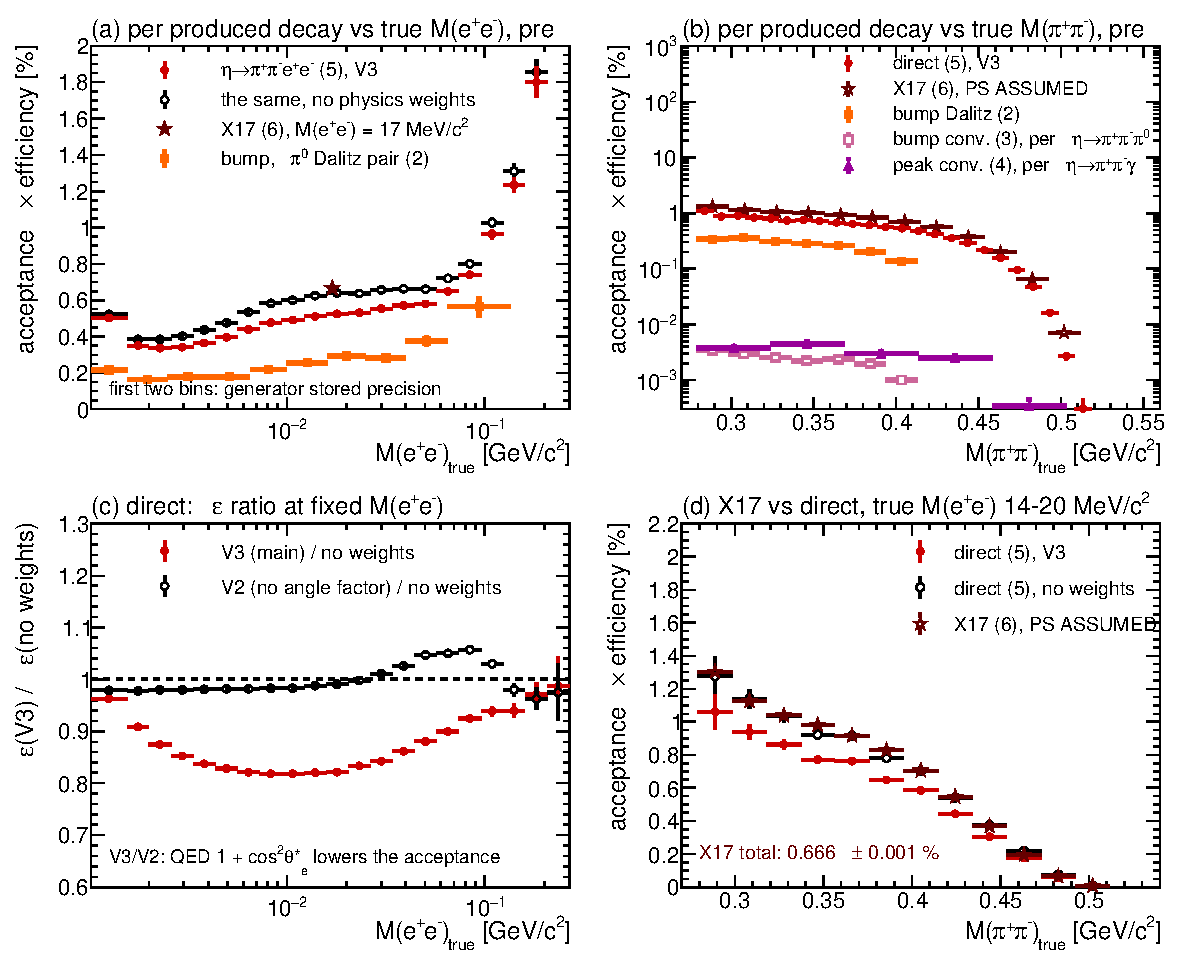
\includegraphics[width=\textwidth]{figs/s5_acc_eff_mass.pdf}
\caption{Acceptance $\times$ efficiency of ``pre'' per produced decay. (a) Against the true \Mee:
direct decay (V3 and without physics weights), bump \piz Dalitz pair, X17. (b) Against the true
\Mpipi for all classes. (c) Ratio V3/no weights and V2/no weights at fixed \Mee: the effect of the
decay angles. (d) X17 against the direct decay at true \Mee 14--20\,\MeVcc.}
\label{fig:s5acc}
\end{figure}

\textbf{Resolution and scale} (Table~\ref{tab:s5res}, Fig.~\ref{fig:s5res}). The difference
reconstructed minus true is fitted with a Gaussian core (iterated in $\pm2\sigma$); the tails are
counted outside $\pm3\sigma$. The reconstructed \Mfour is low by 0.25--0.39\,\% (median ratio)
and has a low-side tail from energy loss and radiation: 6\,\% of the direct decays lie more than
$3\sigma$ below the core. The \Mee resolution comes from the opening-angle measurement (OA
resolution 1.0--1.4$^\circ$): at 17\,\MeVcc the core width is $4.21\pm0.01$\,\MeVcc with a median
shift of $+0.10$\,\MeVcc; 90\,\% of the X17 rows lie in 9.7--24.3\,\MeVcc.

\begin{table}[H]
\centering
\caption{Resolution of \Mfour (reconstructed with corrected momenta minus true), after ``pre''.}
\label{tab:s5res}
\footnotesize
\setlength{\tabcolsep}{4pt}
\begin{tabular}{@{}l rr c r r@{}}
\toprule
 & \multicolumn{2}{c}{$\Delta M_4$ [\MeVcc]} & tail fraction & median & $\Delta M_{\pi\pi}$ core \\
class & median & core $\sigma$ & below / above $3\sigma$ & $M_4/M_{4,\mathrm{true}}$ & $\sigma$ [\MeVcc] \\
\midrule
5 direct      & $-2.12\pm0.02$ & $6.44\pm0.02$ & 0.057 / 0.014 & 0.99614 & $3.49\pm0.01$ \\
6 X17         & $-2.10\pm0.01$ & $6.25\pm0.01$ & 0.063 / 0.013 & 0.99617 & $2.98\pm0.01$ \\
2 bump Dalitz & $-1.47\pm0.22$ & $5.47\pm0.18$ & 0.041 / 0.015 & 0.99694 & $3.13\pm0.12$ \\
3 bump conv.  & $-1.05\pm0.27$ & $5.68\pm0.26$ & 0.033 / 0.020 & 0.99783 & $3.11\pm0.13$ \\
4 peak conv.  & $-1.33\pm0.57$ & $6.13\pm0.40$ & 0.060 / 0.008 & 0.99757 & $3.15\pm0.26$ \\
\bottomrule
\end{tabular}
\end{table}

\begin{figure}[H]
\centering
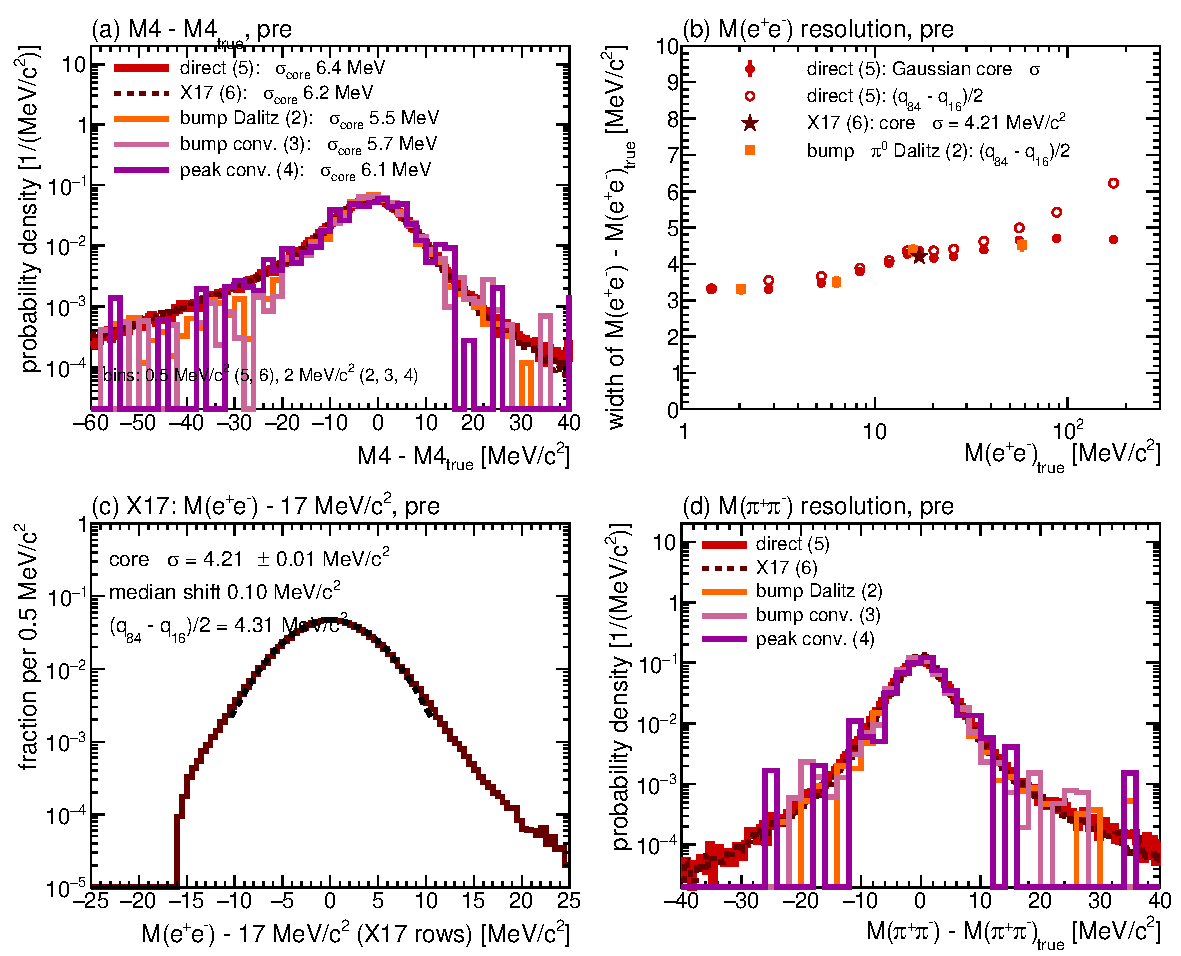
\includegraphics[width=\textwidth]{figs/s5_acc_res.pdf}
\caption{Resolution after ``pre''. (a) $\Mfour-M_{4,\mathrm{true}}$ per class. (b) Width of
$\Mee-M_{ee,\mathrm{true}}$ against the true \Mee. (c) Reconstructed \Mee of the X17 rows minus
17\,\MeVcc. (d) $\Mpipi-M_{\pi\pi,\mathrm{true}}$.}
\label{fig:s5res}
\end{figure}

\textbf{Check of the peak window.} A Gaussian fit of the simulated peak (classes 4+5, V3, 1\,\MeVcc
bins, iterated in $\pm2\sigma$) gives $\mu = 0.54637\pm0.00020$\,\GeVcc and
$\sigma = 6.09\pm0.19$\,\MeVcc, so $\mu\pm1.9\sigma$ = 0.5348--0.5579\,\GeVcc. The fixed window
(0.5333--0.5587) is 1.5\,\MeVcc wider on the low side. Nine fit choices (bin width, fit range)
move the lower edge by $+0.1$ to $+3.2$\,\MeVcc; the direct decay alone ($N_{\mathrm{eff}}$ 171\,000)
reproduces the fixed window within 0.7\,\MeVcc. The fixed window is therefore kept. It holds 0.851
of the simulated peak, $2.262\pm0.070$\,nb (direct $1.207\pm0.003$, conversion $1.054\pm0.070$).

\textbf{The opening angle separates conversions only weakly.} The true OA of a conversion pair is
small (median 0.51$^\circ$), but the reconstructed OA is larger by about 1.6$^\circ$ (median
2.2$^\circ$), because of the OA resolution and the need for two separated tracks. The fraction with
OA$>2^\circ$ is 0.811 (direct), 0.955 (X17), $0.814\pm0.011$ (bump Dalitz), $0.576\pm0.016$ (bump
conversion) and $0.567\pm0.030$ (peak conversion). A cut on \Mee separates about as well:
$\Mee>15$\,\MeVcc keeps 0.50 of the direct decay and 0.02 of the conversion peak.
OA does not separate X17 from the direct decay at the same reconstructed \Mee.

%----------------------------------------------------------------------
\subsection{Cut flow per signal class and background composition}
\label{sec:s5cut}
%----------------------------------------------------------------------
Eight cuts are studied: the four of ``slides'', both pions in the vertex fit,
$\max|z_\pi-z_{\mathrm{vertex}}|<40$\,mm (written $|\Delta z_\pi|$), $\mathrm{MM}_4<2.85$\,\GeVcc and
$p_{T,4}>400$\,\MeVc. For each cut we compute the efficiency $\varepsilon_S$ of the signal and
$\varepsilon_B$ of the background T2 in a window, and
\begin{equation}
Q = \varepsilon_S/\sqrt{\varepsilon_B}.
\end{equation}
$Q$ is the factor by which the cut changes $S/\sqrt{B}$ when $B\gg S$; it needs no luminosity. A cut
carries information if $Q > 1 + \max(0.02, 2\delta Q)$ and is harmful if $Q$ is below the mirror
value. ``Alone'' means the cut on ``pre''; ``N$-$1'' means the cut on top of the other three slides
cuts (for the four other cuts: on top of ``slides''). Errors are from event groups, with pass and
fail rows of one event correlated.

\begin{table}[H]
\centering
\caption{Efficiencies and $Q$ of each cut alone (from ``pre'') in the windows. Peak: $S$ = classes
4+5; bump: $S$ = classes 2+3; X17: $S$ = X17, $B$ = T2 + classes 4+5 (peak window). The error is
in brackets, in units of the last digit.}
\label{tab:s5rank}
\footnotesize
\setlength{\tabcolsep}{3pt}
\begin{tabular}{@{}l ccc ccc cc@{}}
\toprule
 & \multicolumn{3}{c}{peak window} & \multicolumn{3}{c}{bump window} & \multicolumn{2}{c}{X17 (peak window)} \\
cut & $\varepsilon_S$ & $\varepsilon_B$ & $Q$ & $\varepsilon_S$ & $\varepsilon_B$ & $Q$ & $\varepsilon_S$ & $Q$ \\
\midrule
OA$>2^\circ$                     & 0.693(16) & 0.749(8) & 0.801(19) & 0.710(11) & 0.748(7) & 0.820(13) & 0.957 & 1.114(6) \\
$\alpha_{\mathrm{lab}}<50^\circ$ & 0.916(9) & 0.834(7) & 1.003(10) & 0.970(3) & 0.922(4) & 1.010(4) & 0.892 & 0.967(3) \\
$\Mpipi<0.46$                    & 0.981(4) & 0.982(2) & 0.990(4) & 1.000 & 1.000 & 1.000 & 0.980 & 0.989(1) \\
$\alpha_\eta>140^\circ$          & 1.000 & 1.000 & 1.000 & 0.858(10) & 0.947(3) & 0.882(10) & 1.000 & 1.000 \\
pions in vertex fit              & 0.938(7) & 0.806(7) & 1.045(9) & 0.923(6) & 0.784(6) & 1.042(8) & 0.931 & 1.020(4) \\
$|\Delta z_\pi|<40$\,mm          & 0.963(5) & 0.829(7) & 1.058(7) & 0.944(6) & 0.813(6) & 1.047(7) & 0.962 & 1.040(3) \\
$\mathrm{MM}_4<2.85$             & 0.963(5) & 0.904(6) & 1.013(7) & 0.949(5) & 0.886(5) & 1.008(6) & 0.963 & 1.007(3) \\
$p_{T,4}>400$\,\MeVc             & 0.795(12) & 0.588(9) & 1.037(18) & 0.849(8) & 0.712(7) & 1.006(11) & 0.791 & 0.998(6) \\
\midrule
slides (all four), from pre      & 0.606(16) & & 0.790(22) & 0.578(12) & & 0.722(15) & & 1.077(7) \\
\bottomrule
\end{tabular}
\end{table}

What the numbers say (Table~\ref{tab:s5rank}, Figs.~\ref{fig:s5regions} and~\ref{fig:s5rank}):
\begin{itemize}
\item \textbf{Inside the windows the cuts hardly separate signal from the simulated background.}
      Only the two pion-vertex cuts have $Q>1$ significantly ($Q$ = 1.04--1.06 in both windows).
      They select the same rows: given all other cuts, each adds nothing ($Q$ = 0.99--1.02).
      Signal pions come from the primary vertex; 9--15\,\% of the background pion pairs contain a
      $\pi\to\mu$ decay and 28--32\,\% secondary pions.
\item \textbf{OA$>2^\circ$ is harmful for the $\eta$ windows} ($Q = 0.80$ peak, 0.82 bump): it
      removes the signal conversions (classes 3 and 4 keep 0.56--0.57) at the same rate as the
      background conversions. It is informative only for X17 ($Q = 1.114\pm0.006$), whose pairs have a
      median OA of 4.6$^\circ$ against 2.1--2.2$^\circ$ for conversions.
\item \textbf{$\alpha_\eta>140^\circ$} does nothing in the peak window and costs bump signal
      ($Q = 0.882\pm0.010$): it keeps 0.86 of the bump and 0.95 of T2.
\item \textbf{The slides cuts are an \Mfour band-pass} (Fig.~\ref{fig:s5regions}): T2 kept by
      ``slides'' is 0.17 below the bump, 0.64 in the bump window, 0.59 in the peak window, 0.30 in
      0.56--0.70, 0.029 in 0.70--1.00 and $1.8\times10^{-4}$ above 1.00\,\GeVcc. Inside the windows
      they cost 39\,\% (peak) and 42\,\% (bump) of the signal. Their value is a cleaner spectrum
      around the $\eta$ (fits, side bands) and, in data, possibly a smaller CB; neither can be measured
      in this simulation.
\end{itemize}

\begin{figure}[H]
\centering
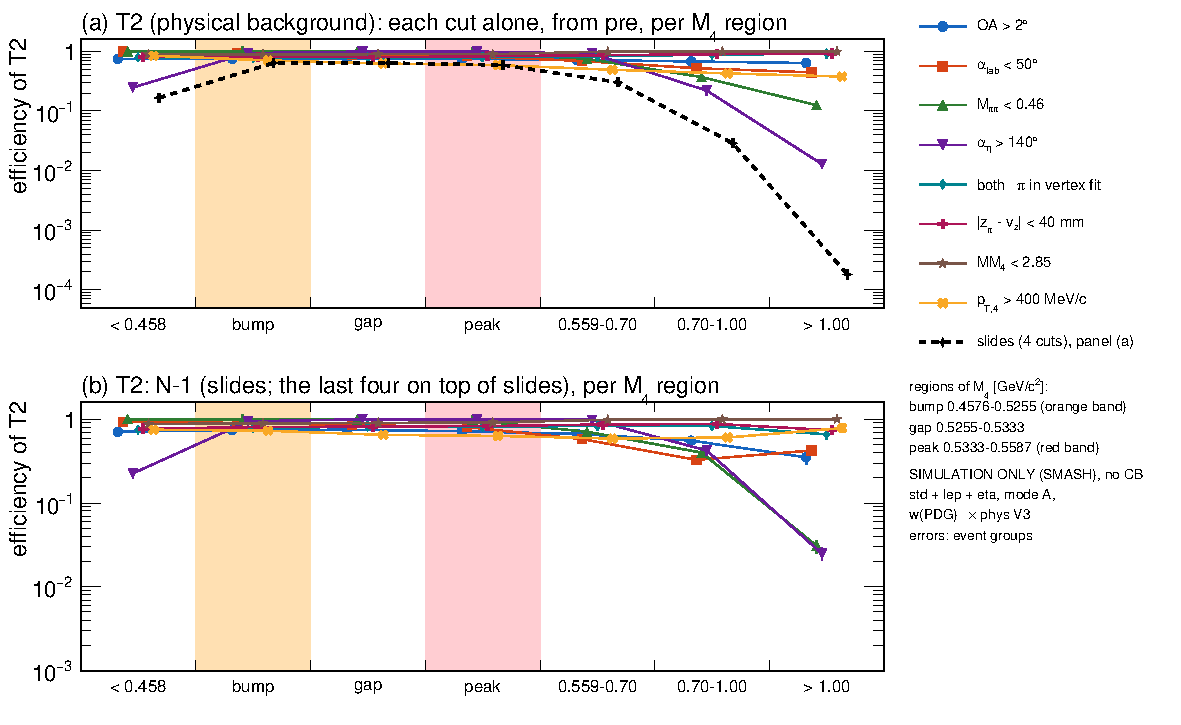
\includegraphics[width=\textwidth]{figs/s5_cut_regions.pdf}
\caption{Efficiency of the physical background T2 per \Mfour region. (a) Each cut alone on
``pre'', and the four slides cuts together (dashed). (b) N$-$1: each cut on top of the other
slides cuts (the last four cuts on top of ``slides''). Errors from event groups.}
\label{fig:s5regions}
\end{figure}

\begin{figure}[H]
\centering
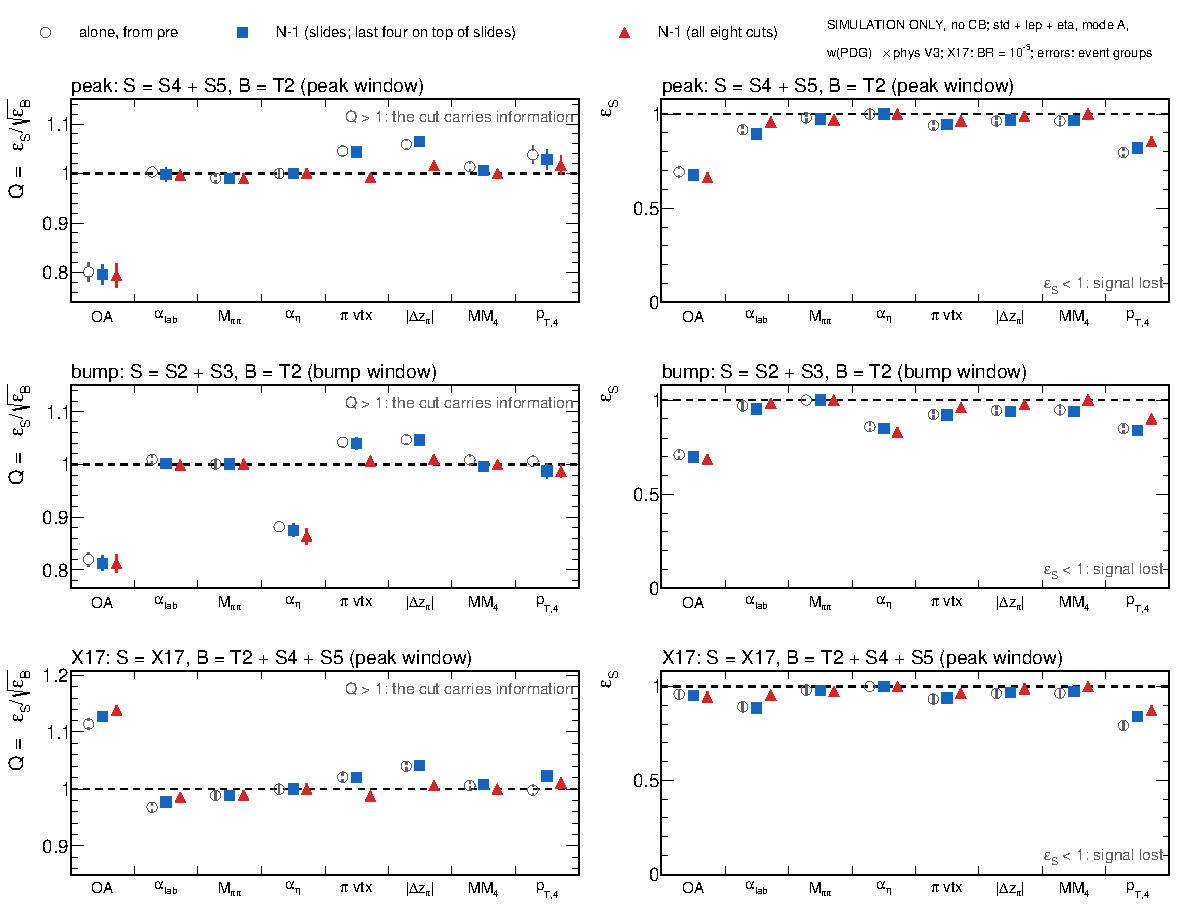
\includegraphics[width=\textwidth]{figs/s5_cut_rank.pdf}
\caption{$Q = \varepsilon_S/\sqrt{\varepsilon_B}$ (left) and $\varepsilon_S$ (right) of the eight cuts
for the peak, the bump and X17 ($\mathrm{BR}=10^{-5}$): alone (open circles), N$-$1 with respect
to ``slides'' (squares), N$-$1 with respect to all eight cuts (triangles).}
\label{fig:s5rank}
\end{figure}

\textbf{Background composition} (Table~\ref{tab:s5comp}). The physical background has the same
make-up in every \Mfour region: \piz Dalitz pairs (L1, 53--60\,\% of T2) and conversion pairs (L3,
28--39\,\%). The pions are mostly both primary (P7, 40--72\,\%) or mixed/secondary (P8, 13--33\,\%);
9--15\,\% of the pion pairs contain a $\pi\to\mu$ decay (P1). $G_\eta$ is 7--10\,\% of T2 around the
$\eta$ and $G_{\mathrm{vec}}$ is negligible. T3 (not in the sum) is 12--20\,\% of T1+T2 near the
$\eta$; 60\,\% of T3 in the peak window are conversion pairs.

\begin{table}[H]
\centering
\caption{Composition after ``pre'' per \Mfour region: $\sigma$ of T1+T2, share of the signal
classes in T1+T2, shares of the groups in T2, and T3, T4 relative to T1+T2 (not in the sum).}
\label{tab:s5comp}
\small
\begin{tabular}{@{}l r r rrr rr@{}}
\toprule
region [\GeVcc] & T1+T2 [nb] & signal share & $G_\eta$ & $G_{\pi^0\mathrm{D}}$ & $G_{\mathrm{conv}}$ & T3 & T4 \\
\midrule
$<0.4576$    & $7.66\pm0.17$ & 0.310(11) & 0.067 & 0.539 & 0.384 & 0.147 & 0.012 \\
bump         & $24.48\pm0.33$ & 0.401(7) & 0.082 & 0.539 & 0.365 & 0.119 & 0.019 \\
gap          & $2.67\pm0.09$ & 0.100(10) & 0.078 & 0.535 & 0.369 & 0.202 & 0.028 \\
peak         & $11.45\pm0.18$ & 0.201(6) & 0.093 & 0.527 & 0.364 & 0.150 & 0.025 \\
0.5587--0.70 & $109.0\pm0.6$ & 0.0013(2) & 0.064 & 0.554 & 0.377 & 0.186 & 0.024 \\
0.70--1.00   & $340.9\pm1.0$ & $<10^{-4}$ & 0.033 & 0.573 & 0.392 & 0.179 & 0.018 \\
$>1.00$      & $205.0\pm0.7$ & 0 & 0.017 & 0.595 & 0.387 & 0.183 & 0.014 \\
\bottomrule
\end{tabular}
\end{table}

\textbf{Statistics.} The std-set signal classes limit every number of this part. In the windows
after ``pre'' class~2 has $N_{\mathrm{eff}} = 1022$, class~3 718 and class~4 225; after all eight
cuts 526, 268 and 79. $G_{\mathrm{vec}}$ and $G_{\mathrm{diff}}$ have $N_{\mathrm{eff}}$ below 150.

%----------------------------------------------------------------------
\subsection{Optimisation for the \texorpdfstring{$\eta$}{eta} peak and bump}
\label{sec:s5opt}
%----------------------------------------------------------------------
\textbf{Targets.} PEAK: classes 4+5 in the peak window. DIRECT: class 5 in the peak window, with
class~4 counted as background. BUMP: classes 2+3 in the bump window. $B$ = all other T1+T2 rows of
the window; a variant adds T3 and T4.

\textbf{Figure of merit and method.} $F = S/\sqrt{S+B}$ with $S$, $B$ in expected rows at
$\Ldata$ (UNCONFIRMED; $F\propto\sqrt{\Ldata}$, the position of the optimum does not depend on it).
Nine cut variables are scanned on grids that contain every named selection: OA$>$ (10 values),
$\alpha_{\mathrm{lab}}<$ (10), $\Mpipi>$ (9), $\Mpipi<$ (10), $\alpha_\eta>$ (8), pions in the
vertex fit (off/on), $|\Delta z_\pi|<40$\,mm (off/on), $\mathrm{MM}_4<$ (8) and $p_{T,4}>$ (6),
$13\,824\,000$ combinations in all. Each window row gets a grid index per variable; the weights are
filled into a 9-dimensional histogram and summed cumulatively along every axis. After that each
cell holds the exact $S$ and $B$ of one combination, and every cell is evaluated (exhaustive
search, no random sampling). The table reproduces the engine sums for all named selections and
direct row loops for 30 random cells (relative difference $<10^{-9}$; 378 checks).

\textbf{Freeze rule} (declared before the search). A candidate must reach $F\ge0.95\,F_{\mathrm{best}}$ on
the full sample and on each half (relative to the best of that half). Among the candidates take
the one with the fewest active cuts, then the one whose worst grid neighbour (each active
threshold moved by one step) has the highest $F$.

\begin{table}[H]
\centering
\caption{Optimisation of the $\eta$ selection (full sample, $\Ldata = 6080.5\,\nbinv$
UNCONFIRMED; errors: simulation statistics). $|\Delta z_\pi|$ stands for $\max|z_\pi-z_{\mathrm{vertex}}|<40$\,mm.
The last two rows are differences of $F$ with the event-group error computed on the difference
itself: the same rows enter both selections, so this error is much smaller than the errors of the
two $F$.}
\label{tab:s5opt}
\small
\begin{tabularx}{\textwidth}{@{}>{\raggedright\arraybackslash}p{3.6cm} L L L@{}}
\toprule
 & PEAK & DIRECT & BUMP \\
\midrule
$F$ at ``pre'' (purity) & $52.12\pm1.51$ (0.198) & $27.83\pm0.23$ (0.105) & $152.7\pm3.0$ (0.396) \\
best cell & $\Mpipi$ 0.32--0.48, $\alpha_\eta>160^\circ$, $|\Delta z_\pi|$, $\mathrm{MM}_4<2.85$
          & $\Mpipi$ 0.30--0.53, $\alpha_\eta>150^\circ$, $|\Delta z_\pi|$, $\mathrm{MM}_4<2.85$
          & $\alpha_{\mathrm{lab}}<70^\circ$, $\Mpipi$ 0.30--0.41, $|\Delta z_\pi|$ \\
$F$ of the best cell (purity) & $56.18\pm1.74$ (0.262) & $29.50\pm0.28$ (0.130) & $157.0\pm3.2$ (0.467) \\
frozen cut & $|\Delta z_\pi|<40$\,mm, $\mathrm{MM}_4<2.85$ & $|\Delta z_\pi|<40$\,mm & none (= pre) \\
$F$ frozen ($F/F_{\mathrm{best}}$) & $54.79\pm1.63$ (0.975) & $28.95\pm0.26$ (0.982) & $152.7\pm3.0$ (0.973) \\
purity, efficiency (frozen) & $0.234\pm0.007$, $0.931\pm0.007$ & $0.119\pm0.002$, $0.963\pm0.001$ & $0.396\pm0.007$, 1 \\
$F$(frozen) $-$ $F$(pre) & $+2.67\pm0.44$ & $+1.12\pm0.10$ & 0 \\
$F$(frozen) $-$ $F$(pre + pions in vertex fit) & $+1.19\pm0.48$ & $+0.58\pm0.09$ & $-1.11\pm0.88$ \\
\bottomrule
\end{tabularx}
\end{table}

\textbf{Results} (Table~\ref{tab:s5opt}, Figs.~\ref{fig:s5profile} and~\ref{fig:s5optcomp}).
\begin{itemize}
\item \textbf{The surface of $F$ is flat.} The plateau ($F\ge0.95\,F_{\mathrm{best}}$) contains, for PEAK:
      OA none or $>1^\circ$; $\alpha_{\mathrm{lab}}<40^\circ$ or looser; $\Mpipi>$ none to 0.34;
      $\Mpipi<0.46$ or looser; any $\alpha_\eta$ up to 170$^\circ$; $\mathrm{MM}_4<2.7$ or looser;
      $p_{T,4}>400$ or looser. The other targets are similar.
\item \textbf{The frozen cuts are better than ``pre'', but only a little.} With the correlated
      error the gain is significant in the simulation: $+2.67\pm0.44$ (5.1\,\%) for PEAK and
      $+1.12\pm0.10$ (4.0\,\%) for DIRECT. Compared with ``pre + pions in vertex fit'' the frozen
      cuts gain $+1.19\pm0.48$ (PEAK) and $+0.58\pm0.09$ (DIRECT). For BUMP no cut is frozen; the
      best cell gains $+4.3\pm1.0$, but this includes the optimisation bias (below).
\item \textbf{The PEAK choice was a knife edge.} ``$|\Delta z_\pi|<40$\,mm'' alone reaches 0.966 of
      $F_{\mathrm{best}}$ on the full sample but 0.9494 on half~B: it missed the half condition by
      0.0006, and the rule added $\mathrm{MM}_4<2.85$ (+1\,\% in $F$). On random halves the rule picks
      ``$|\Delta z_\pi|<40$\,mm'' alone in 167 of 200 cases.
\item \textbf{OA$>2^\circ$ is off the plateau for all three targets}, even for DIRECT, where it keeps
      only 0.81 of the direct decay. Only ``pions in vertex fit'', ``peak nominal'' and (for BUMP)
      ``bump nominal'' are on the plateau (Table~\ref{tab:s5presets}).
\item \textbf{Purity.} The cuts can raise the purity at a small loss of $F$: for BUMP, ``bump
      nominal'' gives 0.456 and the best purity on the plateau ($\alpha_{\mathrm{lab}}<40^\circ$,
      $\Mpipi>0.32$, $|\Delta z_\pi|$) 0.496, against 0.396 at ``pre''. These purity choices are not
      stable between halves (the most frequent half pick occurs in only 32--61 of 200 cases).
\end{itemize}

\begin{table}[H]
\centering
\caption{Named selections: $F/F_{\mathrm{best}}$ per target (errors about 3\,\% PEAK, 1\,\% DIRECT,
2\,\% BUMP; $\Ldata$ UNCONFIRMED).}
\label{tab:s5presets}
\small
\begin{tabular}{@{}l ccc@{}}
\toprule
selection & PEAK & DIRECT & BUMP \\
\midrule
pre                     & 0.928 & 0.943 & 0.973 \\
pre + OA$>2^\circ$       & 0.748 & 0.889 & 0.806 \\
pre + pions in vertex fit & 0.954 & 0.962 & 0.980 \\
slides                  & 0.730 & 0.889 & 0.716 \\
old code                & 0.784 & 0.848 & 0.877 \\
peak nominal            & 0.941 & 0.953 & 0.979 \\
bump nominal            & 0.732 & 0.783 & 0.977 \\
\bottomrule
\end{tabular}
\end{table}

\begin{figure}[H]
\centering
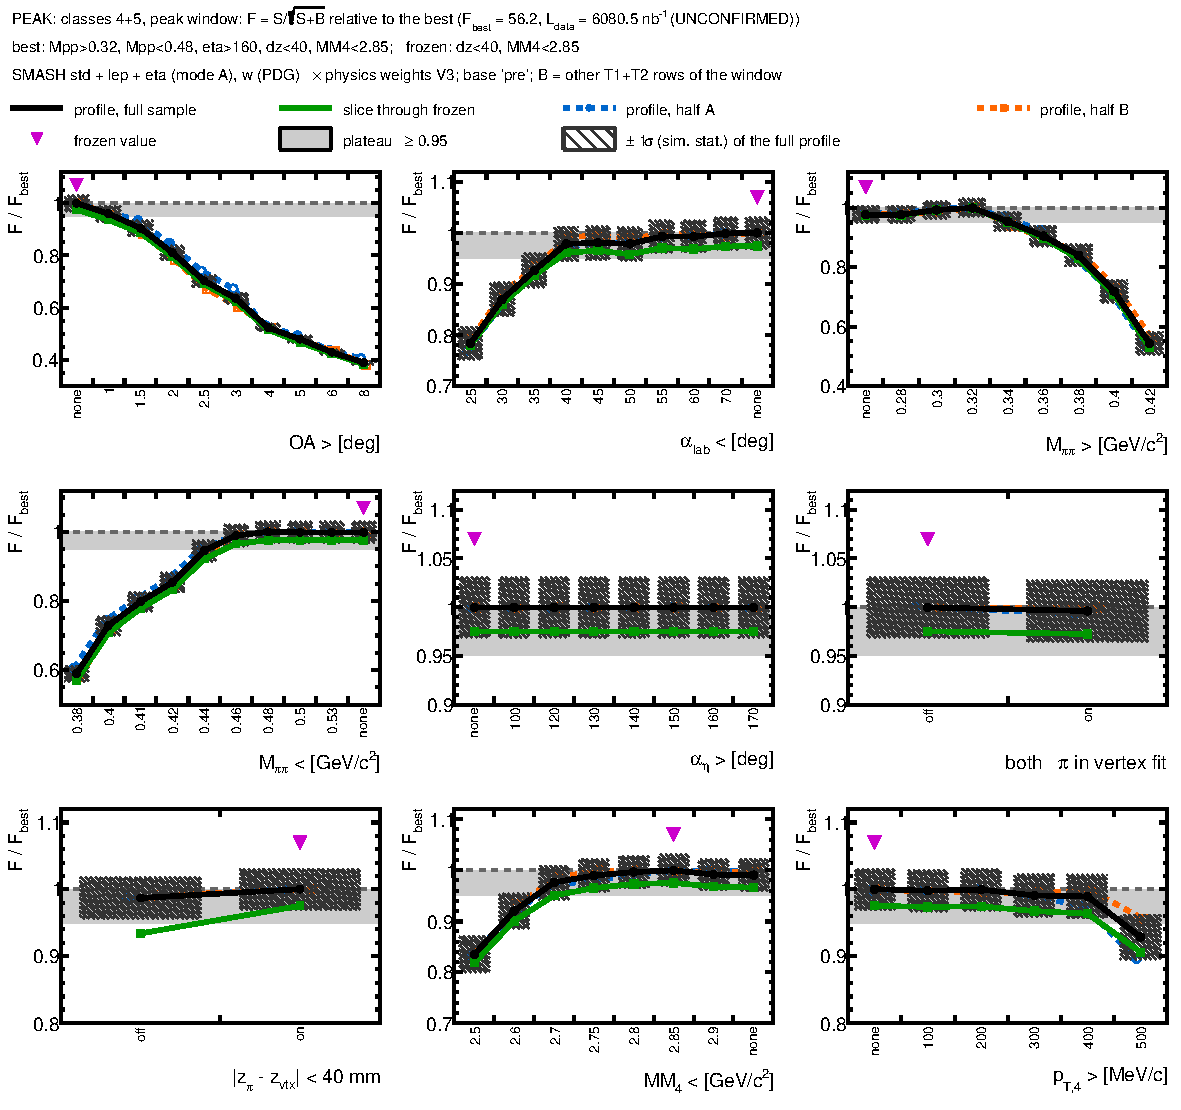
\includegraphics[width=\textwidth]{figs/s5_opt_eta_profile_peak.pdf}
\caption{PEAK target: $F/F_{\mathrm{best}}$ against each cut variable. Profile = the best $F$ over
all other variables at a fixed value (full sample, black; half A and half B relative to their
own best, dashed). The hatched band is the $\pm1\sigma$ statistical error of the full-sample $F$
at each profile point; differences between neighbouring points are much more precise, because
the rows are shared. Green: slice through the frozen point. Grey band: plateau
($\ge0.95$). Triangle: frozen value. $\Ldata = 6080.5\,\nbinv$ (UNCONFIRMED).}
\label{fig:s5profile}
\end{figure}

\begin{figure}[H]
\centering
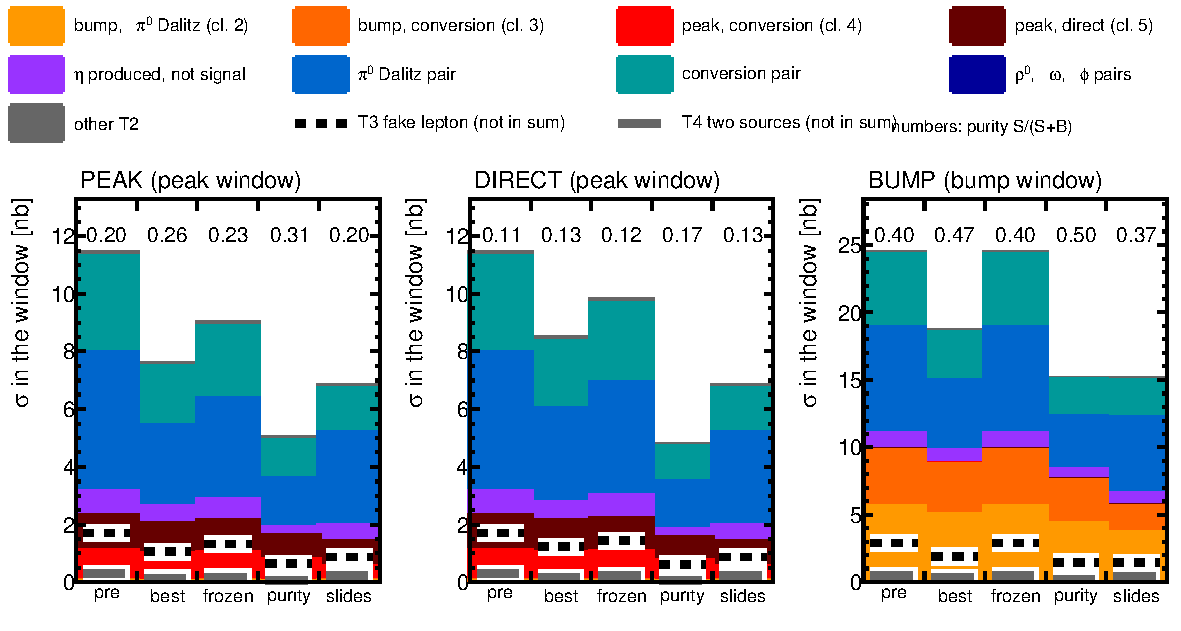
\includegraphics[width=\textwidth]{figs/s5_opt_eta_composition.pdf}
\caption{Content of the target window by group, $\sigma$ in nb, for ``pre'', the best cell, the
frozen cut, the best purity on the plateau and ``slides'' (stacked: T1+T2 groups). T3 (dashed
line) and T4 (dash-dotted line) are drawn at their own level and are not in the stack. Numbers
above the bars: purity $S/(S+B)$.}
\label{fig:s5optcomp}
\end{figure}

\textbf{Split-half check of the optimisation bias.} The rows are split by event group into two
halves (half A = even group number, half B = odd; each half weighted by 2). The search is run on
one half and the chosen cell is evaluated on the other. The bias is $F$(optimising half) $-$
$F$(other half), averaged over both directions, because a single direction also contains the
difference between the halves at fixed cuts (PEAK at ``pre'': $F_A = 51.28$, $F_B = 52.97$).
\begin{center}
\small
\begin{tabular}{@{}l ccc ccc@{}}
\toprule
 & \multicolumn{3}{c}{100 random splits (mean $\pm$ error of the mean)} & \multicolumn{3}{c}{deterministic split (A/B)} \\
target & best cell & freeze rule & purity rule & best cell & freeze rule & purity rule \\
\midrule
PEAK   & $+2.71\pm0.11$\,\% & $+0.68\pm0.09$\,\% & $+1.55\pm0.15$\,\% & $+2.08$\,\% & $+1.77$\,\% & $+0.61$\,\% \\
DIRECT & $+0.75\pm0.05$\,\% & $+0.06\pm0.01$\,\% & $+0.80\pm0.07$\,\% & $+0.37$\,\% & 0.00\,\% & $+1.65$\,\% \\
BUMP   & $+1.10\pm0.07$\,\% & $+0.08\pm0.01$\,\% & $+1.64\pm0.09$\,\% & $+0.65$\,\% & 0.00\,\% & $+1.30$\,\% \\
\bottomrule
\end{tabular}
\end{center}
The gain of the best cell over ``pre'' (PEAK $+7.8$\,\%, DIRECT $+6.0$\,\%, BUMP $+2.8$\,\%) is partly
this bias; the freeze rule reduces it to below 1\,\%. Single directions range from $-7.7$ to
$+9.2$\,\%: this is the noise between halves, set by the std set. The limiting components are
class~4 ($N_{\mathrm{eff}}$ 209 at the frozen PEAK cut; it gives almost all of the 3.0\,\% error of $F$),
the std part of $B$ ($N_{\mathrm{eff}}$ 924) and, for BUMP, the signal itself ($N_{\mathrm{eff}}$ 1739).

\notebox{\textbf{Frozen $\eta$ selections} (\code{plots/eta_sim/}\allowbreak\code{tables/s5_opt_eta_frozen.txt}):
PEAK = pre + $|\Delta z_\pi|<40$\,mm + $\mathrm{MM}_4<2.85$\,\GeVcc; DIRECT = pre + $|\Delta z_\pi|<40$\,mm;
BUMP = pre. \textbf{Caveat for data:} $|\Delta z_\pi|$ needs the $z$ of the pion tracks, which the
compact data rows (\code{ScanEngine.h}) do not have yet. The data-ready alternative on the plateau is
``pre + pions in vertex fit'' ($F/F_{\mathrm{best}}$ = 0.954, 0.962, 0.980). Without CB the
simulation-only optimum may be looser than the data optimum, since the CB and its subtraction
add to the variance and the cuts also reduce the CB.}

%----------------------------------------------------------------------
\subsection{A selection aimed at X17 and its expected limit}
\label{sec:s5x17}
%----------------------------------------------------------------------
\textbf{The X17 line.} In the peak window after ``pre'', the reconstructed \Mee of the X17 rows has
a mean of $17.25\pm0.01$\,\MeVcc and a Gaussian core of $\sigma = 4.04\pm0.01$\,\MeVcc; 93.3\,\% lie
within $\pm2\sigma$. The width depends on the opening angle: 4.5\,\MeVcc for OA$<2^\circ$,
3.3\,\MeVcc for OA$>8^\circ$; the mean moves from 13.6 (OA$<3^\circ$) to 20.3\,\MeVcc
(OA$>8^\circ$), so an OA cut reshapes the line. In \Mfour the X17 rows have mean 546.6\,\MeVcc and
$\sigma = 5.9$\,\MeVcc; 85.7\,\% of them lie in the peak window.

\textbf{Figure of merit.} The expected 90\,\% CL upper limit on
$\mathrm{BR}\equiv\mathrm{BR}(\eta\to\pipi X17)\,\mathrm{BR}(X17\to\ee)$ from counting in a window,
for $\mathrm{BR}=0$:
\begin{equation}
\mathrm{UL} = \sqrt{\mathrm{UL}_{\mathrm{stat}}^2 + \left(1.645\,\sigma_{B,\mathrm{MC}}/s_1\right)^2},
\qquad \mathrm{UL}_{\mathrm{stat}} = s_{\mathrm{up}}(B)/s_1 .
\label{eq:s5ul}
\end{equation}
Here $s_1$ is the number of selected X17 rows per unit BR and $B$ the background rows (T1 without
X17, plus T2), both at \Ldata; $s_{\mathrm{up}}(B)$ is the CLs upper limit on the signal for an
observed count equal to $B$ (continuous Poisson, about $1.645\sqrt{B}$ for large $B$); and
$\sigma_{B,\mathrm{MC}}$ is the simulation (event-group) error of $B$. The second term is there
because a counting analysis takes $B$ from this simulation. $\mathrm{UL}_{\mathrm{stat}}$ alone is
the limit with the background known exactly: a statistical limit only.

\textbf{Two versions.} The first optimisation (v1, used by the blind test of
Sect.~\ref{sec:s5blind}) used $\mathrm{UL}_{\mathrm{stat}}$ and also optimised the edges of the
\Mfour window. A review found two problems: the MC error of $B$ ($\pm307$ rows) is larger than
the statistical term, and the \Mfour window was to stay fixed for all parts of the study. The
optimisation was therefore repeated (v2) with Eq.~(\ref{eq:s5ul}) and the fixed peak window.
Method: coordinate descent over \Mee window, OA (lower and upper), $\alpha_{\mathrm{lab}}$,
\Mpipi (lower and upper), $\alpha_\eta$ and pions in the vertex fit; in each step the loosest value
within 2\,\% of the step minimum is taken. Two different starting points end at the same optimum.

\begin{table}[H]
\centering
\caption{X17 selections after ``pre''. Rows at $\Ldata = 6080.5\,\nbinv$ (UNCONFIRMED). UL in
units of $10^{-6}$; ``shape'': binned likelihood of \Mee 2--62\,\MeVcc in the \Mfour window with a
Gaussian X17 line (background shape from the simulation, normalisation known or free).
$Z$: Asimov significance for $\mathrm{BR}=10^{-5}$ with $B$ known.}
\label{tab:s5x17}
\small
\begin{tabularx}{\textwidth}{@{}L >{\raggedright\arraybackslash}p{4.4cm} >{\raggedright\arraybackslash}p{4.4cm}@{}}
\toprule
 & v1 (blind test) & v2 (frozen) \\
\midrule
cuts in addition to ``pre'' & \Mfour 0.5330--0.5555, \Mee 13.0--26.5, pions in vertex fit
                            & \Mfour 0.5333--0.5587, \Mee 15.5--24.5, pions in vertex fit \\
X17 rows per unit BR, $s_1$  & $2.727\times10^{7}$ & $2.127\times10^{7}$ \\
X17 rows at $\mathrm{BR}=10^{-5}$ & 272.7 & 212.7 \\
background $B$ [nb] ($N_{\mathrm{eff}}$) & $1.333\pm0.051$ (696) & $0.878\pm0.039$ (501) \\
background rows $B\pm\sigma_{B,\mathrm{MC}}$ & $8108\pm307$ & $5342\pm239$ \\
$\mathrm{UL}_{\mathrm{stat}}$ (B known exactly) & 5.48 & 5.71 \\
$\mathrm{UL}$, Eq.~(\ref{eq:s5ul}) (with the MC error of $B$) & 19.3 & 19.3 \\
shape, $B$ known / normalisation free & 4.85 / 5.40 & 4.96 / 5.54 \\
$Z$($\mathrm{BR}=10^{-5}$), $B$ known / with $\sigma_{B,\mathrm{MC}}$ & 3.01 / 0.85 & 2.89 / 0.85 \\
\bottomrule
\end{tabularx}
\end{table}

\textbf{Results} (Table~\ref{tab:s5x17}, Fig.~\ref{fig:s5x17shape}).
\begin{itemize}
\item \textbf{The MC error of the background sets the limit.} With the MC term the expected limit is
      $1.93\times10^{-5}$ for both selections, 3.4--3.5 times $\mathrm{UL}_{\mathrm{stat}}$. The
      re-optimisation gains nothing: the v1 cuts give $1.933\times10^{-5}$, the v2 cuts
      $1.931\times10^{-5}$. ``slides'' with the same \Mee window gives $2.15\times10^{-5}$.
\item \textbf{Where the MC error comes from.} At the v2 optimum the variance of $B$ comes from
      $G_{\pi^0\mathrm{D}}$ (60\,\%; lep set, $N_{\mathrm{eff}}$ 313), $G_{\mathrm{conv}}$ (24\,\%; 19 std
      rows, $N_{\mathrm{eff}}$ 18) and $G_\eta$ (12\,\%; $N_{\mathrm{eff}}$ 29). One std row stands for 27.5
      expected data rows.
\item \textbf{Cuts.} The \Mee window keeps 0.62 of X17 and 0.094 of $B$; the pion-vertex cut keeps
      0.93 of X17 and 0.82 of $B$. OA, $\alpha_{\mathrm{lab}}$, \Mpipi and $\alpha_\eta$ cuts do not
      lower the limit: at \Mee 12--22\,\MeVcc the OA medians of X17 (4.9$^\circ$), the direct decay
      (4.6$^\circ$) and $G_{\pi^0\mathrm{D}}$ (5.2$^\circ$) are about the same.
\item \textbf{Composition of $B$} (v1): $G_{\pi^0\mathrm{D}}$ 0.56, direct decay (class 5) 0.18,
      $G_{\mathrm{conv}}$ 0.12, $G_\eta$ 0.08, class 4 0.03. The direct decay is an irreducible
      background under the line.
\item \textbf{Split halves} (v2 figure of merit): the optimum of half A gives 28.1 on A and 30.2 on
      B, that of half B 24.4 and 28.1 (in $10^{-6}$; each half has a $\sqrt2$ larger MC error). The
      bias is 7--15\,\%: with the MC term the figure of merit is itself noisy, and the optimum
      (\Mee 13--27.5 on half A, 15.5--23.5 on half B) is not better determined than in v1.
\end{itemize}

\begin{figure}[H]
\centering
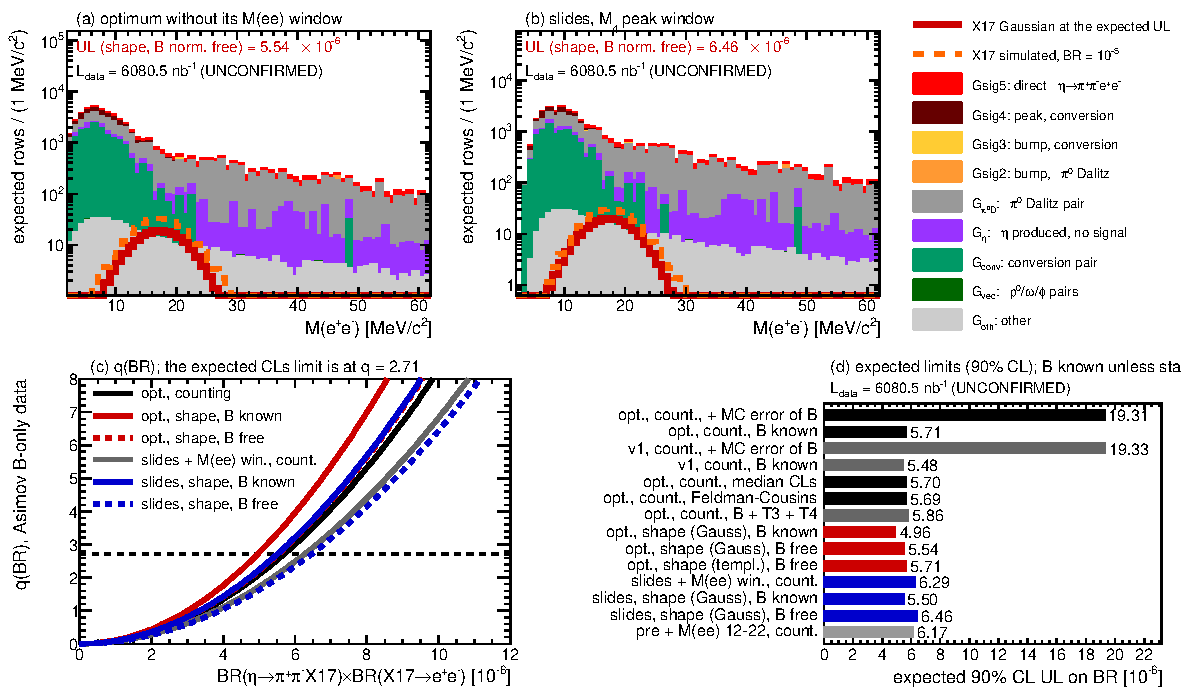
\includegraphics[width=\textwidth]{figs/s5_opt_x17_shape.pdf}
\caption{X17 search, expected rows at $\Ldata = 6080.5\,\nbinv$ (UNCONFIRMED). (a) \Mee at the v2
optimum without its \Mee window, stacked background groups, X17 as a Gaussian at the expected limit
of the shape fit and as the simulated template at $\mathrm{BR}=10^{-5}$. (b) The same for
``slides''. (c) Test statistic $q(\mathrm{BR})$ on Asimov background-only data; the expected
CLs limit is at $q = 2.71$. (d) Expected 90\,\% CL limits; ``B known'' ignores the MC error of $B$.}
\label{fig:s5x17shape}
\end{figure}

\notebox{\textbf{Frozen X17 selection v2} (\code{plots/eta_sim/}\allowbreak\code{tables/s5_opt_x17_frozen.txt}; v1 kept in
\code{s5_opt_x17_frozen_v1.txt}): pre + peak window + $15.5\le\Mee<24.5$\,\MeVcc + both pions in
the vertex fit. Expected 90\,\% CL limit by counting $1.9\times10^{-5}$ including the MC error of
the background; $5.7\times10^{-6}$ if the background were known exactly. These numbers assume
$\Ldata = 6080.5\,\nbinv$ (UNCONFIRMED), no CB, the SMASH background and phase space for X17.}

%----------------------------------------------------------------------
\subsection{Blind test of the signal extraction and of the X17 search}
\label{sec:s5blind}
%----------------------------------------------------------------------
The extraction methods planned for the data were tested on simulated pseudo-data whose true
content was hidden from the analyst until the procedure was frozen.

\textbf{Preparation.}
\begin{enumerate}
\item \textbf{Split.} The rows are split by event group: half A (even group number) gives the
      templates, half B (odd) gives the pseudo-data. Every row of an event goes to the same half.
\item \textbf{Templates}: half A with weights $\times2$, histograms of \Mfour (1\,\MeVcc bins) per
      component and selection (PEAK, DIRECT, BUMP of Sect.~\ref{sec:s5opt} and the v1 X17 selection),
      exact window sums, and \Mee and $\Mfour\times\Mee$ for X17.
\item \textbf{$\eta$ pseudo-data}: 200 toys at $L_{\mathrm{toy}} = \Lsim/2 = 110.525\,\nbinv$ from a
      Poisson bootstrap of half B per event group. An event with largest row weight $w_g$ enters
      $n\sim\mathrm{Poisson}(w_g)$ times; in each copy one uniform $u$ is drawn and each row with
      $w_r/w_g>u$ is kept, so that every row has the expected multiplicity $w_r$. Only T1+T2 rows
      are used. A check with 4000 toys gave toy variance / predicted variance = 0.95--1.06; the sum
      of the squared pulls of the variances over the 21 regions was 36.8. Repeated with eight further
      random seeds, this sum is 9.1--35.7, on average $20.7\pm10.1$ over all nine runs (21 expected; the
      spread is wider than for 21 independent entries because the selections share rows), and the
      variance ratio stays within 0.94--1.06: the bootstrap reproduces the variances, the value 36.8 is
      a fluctuation.
\item \textbf{X17 pseudo-data}: 1500 toys at \Ldata (UNCONFIRMED), parametric: in each cell of
      $\Mfour\times\Mee$ signal and background are drawn as Poisson numbers around the half-B
      expectation ($\times2\times\Ldata/\Lsim$). BR $\in\{0, 1, 3, 10, 30\}\times10^{-6}$, 300 toys
      each, shuffled, with random ids.
\item \textbf{Sealed key}: true rows per toy, group and region; the expectation of half B per
      toy, called $\mu$, is the quantity a measurement would estimate.
\end{enumerate}
For the weight rules~v2 the $\eta$ and X17 toys were drawn again with the same seed. Because
the weights changed, the random draws differ from those of rules~v1, so the biases and pulls
moved within their statistical errors (by up to 2.3 standard deviations).

\textbf{Methods} (frozen before any yield was computed on the pseudo-data). Peak yield: M1 =
Gaussian (fixed at 0.5460\,\GeVcc, 6.7\,\MeVcc) + second-order polynomial, calibrated with the
response to the half-A peak template; M2 = template fit (free normalisations of peak, bump and
background templates, binned Poisson likelihood with the template variance added); M2b = M2
with the background split into $G_\eta$ and the rest; M2d = M2 with the peak split into class 5
(free) and class 4 (constrained to its half-A value $\pm$ its MC error); M3 = linear side bands
(7.8\,\MeVcc on each side) with the signal leakage $\lambda$ into the side bands corrected,
$S = [N_{\mathrm{win}} - (N_L+N_U)/2\cdot25.4/7.8]/(1-\lambda)$; M3c = M3 with the curvature of
the background taken from half A. Bump yield: B1 = bifurcated Gaussian + $\eta$ Gaussian +
polynomial; B2 = the bump of M2; B3 = edge step in \Mfour; B4 = side band 0.5665--0.70 with
the background shape from half A. Direct yield: M2d, and D5 = split at $\Mee = 10$\,\MeVcc with a
$2\times2$ unfolding. X17: X1 = fit of \Mee in the window with free normalisations of the direct
decay and the rest; X2 = X1 with the raw half-A template; X3 = X1 on 8--40\,\MeVcc; X4 = X1 with
the direct-decay normalisation constrained to $1\pm0.10$; X5 = counting with $B$ from half A.
X4 and X5 were added after the X1 results were seen (declared, before their own results). An
example toy with the fits is shown in Fig.~\ref{fig:s5toy}.

\begin{figure}[H]
\centering
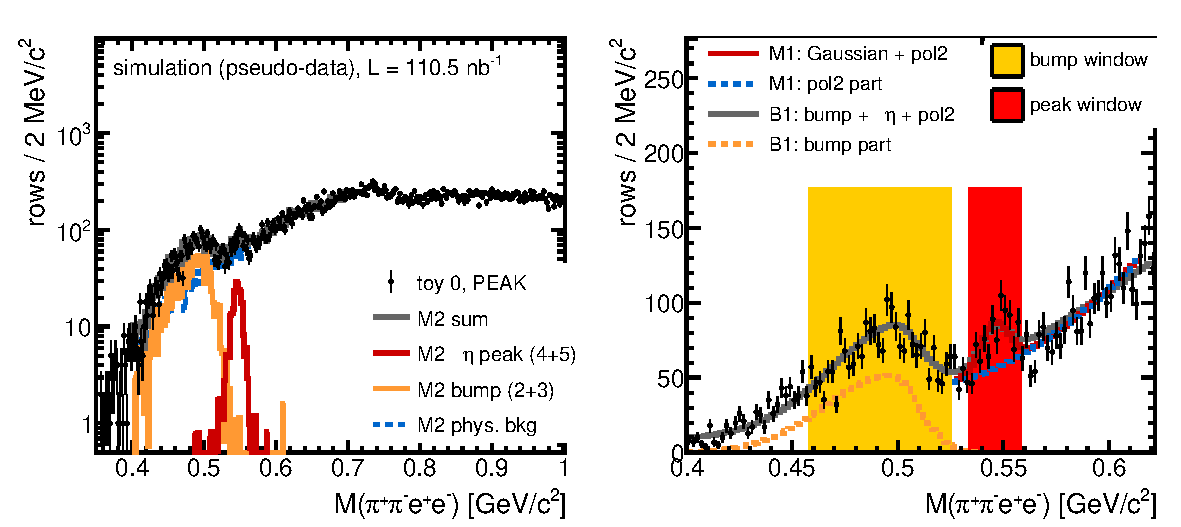
\includegraphics[width=\textwidth]{figs/s5_blind_ana_toy0_PEAK.pdf}
\caption{One $\eta$ toy (pseudo-data, $L = 110.5\,\nbinv$, PEAK selection). Left: \Mfour with
the components of the template fit M2. Right: zoom with the Gaussian + polynomial fit M1 and the
bump fit B1, with the bump and peak windows.}
\label{fig:s5toy}
\end{figure}

\textbf{What a bias means here.} The templates (half A) and the pseudo-data (half B) are two
statistically independent copies of the same model. The truth of half B differs from half A by
MC fluctuations: peak (PEAK selection) $241.4$ against $224.1\pm10.3$ rows (+7.7\,\%), bump (BUMP)
1095.6 against $1046.1\pm35.7$ (+4.7\,\%), class 5 (DIRECT) 128.88 against $128.00\pm0.48$, class 4
(DIRECT) 118.5 against $106.2\pm10.5$ (+11.5\,\%). All toys share this difference. A method bias
can therefore be resolved only beyond the common MC error, which is $\pm$11--15\,\% for the peak and
$\pm$4.5--5\,\% for the bump.

\begin{table}[H]
\centering
\caption{Blind test, $\eta$ yields (200 toys). Bias = $\langle Y\rangle - \mu$ with the error of the
mean over toys and the common MC error (template and parent sample). Pull = $(Y-\mu)/\sigma_{\mathrm{tot}}$
with the error quoted by the analyst (mean/rms). Coverage: fraction of toys with
$|Y-\mu|\le\sigma_{\mathrm{tot}}$ (nominal 0.683).}
\label{tab:s5blind}
\footnotesize
\setlength{\tabcolsep}{4pt}
\begin{tabular}{@{}l l r r c c@{}}
\toprule
yield, selection ($\mu$) & method & bias [rows] & relative & pull & coverage \\
\midrule
peak, PEAK (241.4)  & M1 Gauss + pol2   & $+7.4\pm2.9\pm31.3$  & $+3.1$\,\%  & $+0.17$ / 0.96 & 0.72 \\
                    & M2 template fit   & $+3.4\pm2.0\pm27.5$  & $+1.4$\,\%  & $+0.08$ / 0.80 & 0.77 \\
                    & M2b               & $+10.4\pm2.2\pm30.6$ & $+4.3$\,\%  & $+0.26$ / 0.82 & 0.74 \\
                    & M3 side bands     & $-51.0\pm3.9\pm45.3$ & $-21.1$\,\% & $-0.86$ / 0.93 & 0.53 \\
                    & M3c               & $-124.5\pm3.9\pm56.9$ & $-51.6$\,\% & $-1.82$ / 0.80 & 0.16 \\
\midrule
bump, BUMP (1095.6) & B4 side band & $+42.3\pm3.9\pm54.9$ & $+3.9$\,\% & $+0.61$ / 0.79 & 0.66 \\
                    & M2 template fit   & $+84.5\pm3.4\pm49.7$ & $+7.7$\,\%  & $+1.34$ / 0.76 & 0.31 \\
                    & B1 parametric     & $+59.0\pm7.1\pm78.6$ & $+5.4$\,\%  & $+0.56$ / 0.96 & 0.66 \\
                    & B3 edge step      & $+13.8\pm13.3\pm171.5$ & $+1.3$\,\% & $+0.01$ / 0.86 & 0.76 \\
\midrule
direct, DIRECT (128.9) & M2d (cl.\ 4 constr.) & $+26.6\pm2.2\pm31.0$ & $+20.6$\,\% & $+0.68$ / 0.79 & 0.62 \\
                    & D5 (\Mee split)   & $+40.5\pm3.9\pm39.3$ & $+31.4$\,\% & $+0.70$ / 0.96 & 0.61 \\
\bottomrule
\end{tabular}
\end{table}

\textbf{$\eta$ results} (Table~\ref{tab:s5blind}, Fig.~\ref{fig:s5bias}).
\begin{itemize}
\item \textbf{Peak.} The template fit M2 and the calibrated Gaussian fit M1 find the peak within
      +1 to +6\,\% in all three selections, well inside the common MC error. Per toy they differ by
      about 12\,\% (rms 29 rows), so a difference of that size between them in data is normal.
      M2b is 3--8\,\% above M2 every time.
\item \textbf{Linear side bands (M3) lose the peak}, because the background is convex under it and
      17\,\% of the signal leaks into the side bands. Two independent realisations of the MC noise
      measure this: the half-B toys give $-21$\,\%, $-13$\,\%, $-16$\,\% and the exact half-A sums
      (Asimov) $-40$\,\%, $-43$\,\%, $-46$\,\% (PEAK, DIRECT, BUMP); the mean is about $-30\pm14$\,\%.
      The MC-calibrated version M3c over-corrects ($-44$ to $-52$\,\%), because the curvature from
      the simulation is itself noisy.
\item \textbf{Bump.} B4 is closest (+3 to +4\,\%); the template fit agrees within 3--8\,\%; the
      parametric fit B1 comes out 5--10\,\% high; the edge step B3 is unbiased but has 15--17\,\%
      statistical error.
\item \textbf{Direct decay alone.} \Mfour cannot separate class 5 from class 4. M2d gives
      class 4 = 105.4 (truth 118.5) and therefore class 5 too high by the same amount
      ($26.6 = 13.5 + 13.1$ rows). The split is limited by the simulation statistics of the
      conversion peak ($N_{\mathrm{eff}}\approx100$ in a half).
\item \textbf{Errors.} The event-group errors describe the spread of the toys: the ratio rms/error
      is 0.93--1.08 for M1, M3, B1, B3 and D5 and 0.90--1.06 for the template fits and B4, so the
      errors are adequate. The common MC error is not in the per-toy error and must be added.
\end{itemize}

\begin{figure}[H]
\centering
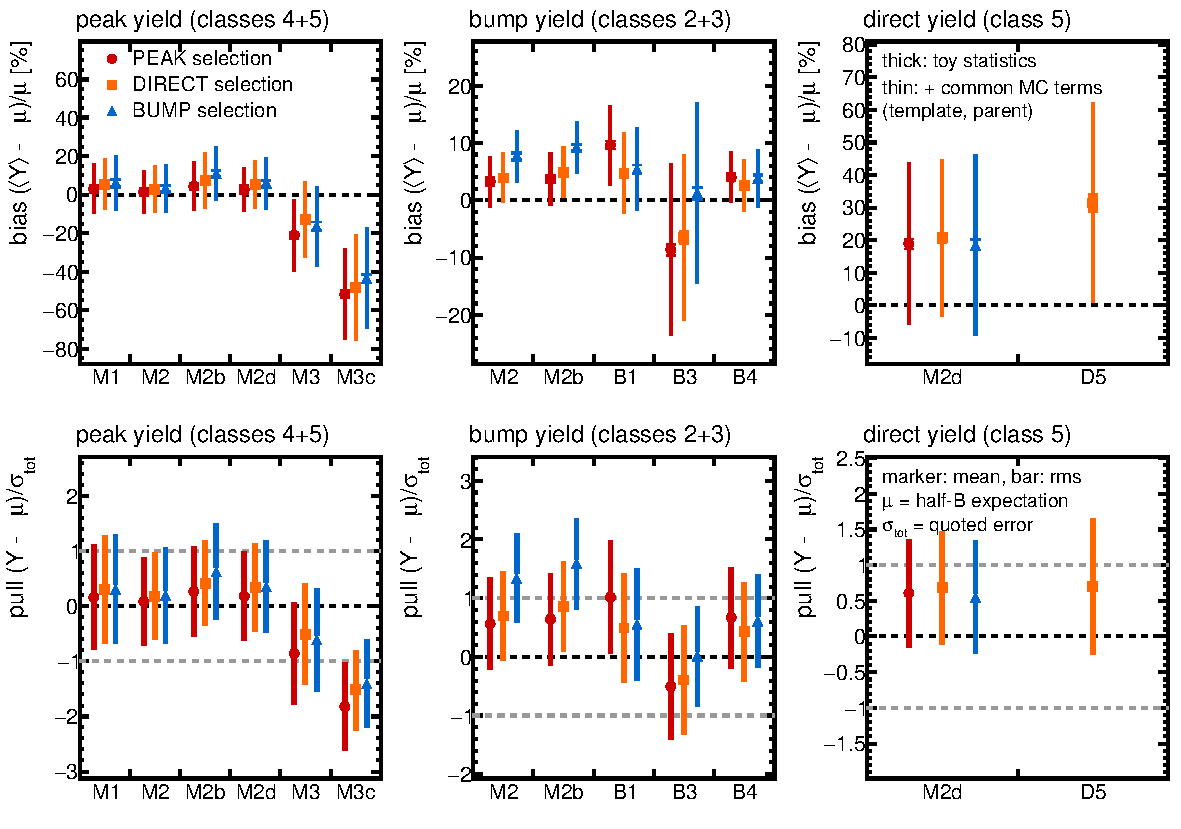
\includegraphics[width=\textwidth]{figs/s5_blind_eval_eta_bias.pdf}
\caption{Blind test, $\eta$ yields. Top: relative bias $(\langle Y\rangle-\mu)/\mu$ per method and
selection; thick bars: toy statistics, thin bars: including the common MC terms. Bottom: pull
$(Y-\mu)/\sigma_{\mathrm{tot}}$, marker = mean, bar = rms.}
\label{fig:s5bias}
\end{figure}

\textbf{X17 results} (Table~\ref{tab:s5blindx}, Figs.~\ref{fig:s5side} and~\ref{fig:s5x17lin}).
Each std row of half B stands for about 55 expected data rows. The background of every X17 toy
is therefore the unsmoothed half-B content, with single-bin spikes of 50--200 rows that all toys
share and that differ from half A (Fig.~\ref{fig:s5side}).
\begin{itemize}
\item Every estimator follows the injected BR with a slope of 0.98--1.02.
\item The zero point is shifted, by the same amount in all toys: it is set by how well the
      background under the line is known. Counting with the half-A background (X5) closes exactly:
      the predicted shift $(B_B-B_A)/s_1 = (7947.8-8268.2)/2.725\times10^{7} = -11.76\times10^{-6}$
      is measured as $-11.66\pm0.19\times10^{-6}$ at $\mathrm{BR}=0$.
\item Only estimators whose error contains this background uncertainty give valid limits (X1, X4,
      X5 cover the true BR at every BR). Their median limits at $\mathrm{BR}=0$ are
      $2.1$--$6.2\times10^{-5}$, 4--11 times the $\mathrm{UL}_{\mathrm{stat}}$ of v1, and consistent
      with the $1.9\times10^{-5}$ of Eq.~(\ref{eq:s5ul}).
\item Estimators with a small error (X2, X3, X1 with the statistical error only) exclude the true
      BR. No estimator claimed a $3\sigma$ signal at $\mathrm{BR}=0$, but only because the common shift
      happens to be negative: with the opposite sign X2 and X3 would claim one in 100\,\% and 98\,\%
      of the toys.
\end{itemize}

\begin{table}[H]
\centering
\caption{Blind test, X17 (1500 toys at $\Ldata = 6080.5\,\nbinv$, UNCONFIRMED; BR in $10^{-6}$).
Offset: mean extracted BR at injected $\mathrm{BR}=0$. Coverage: fraction of toys whose UL is above
the injected BR. X1--X3 were frozen; X4 (X1 with the direct-decay normalisation $a_D$ constrained) and X5
(counting) were added after the freeze.}
\label{tab:s5blindx}
\footnotesize
\setlength{\tabcolsep}{4pt}
\begin{tabular}{@{}l c c c c@{}}
\toprule
estimator & offset at 0 & slope & median UL at 0 (16--84\,\%) & UL coverage at 0 / 3 / 10 / 30 \\
\midrule
X1 window fit         & $-72.7\pm0.5$ & $1.004\pm0.021$ & 31.2 (28.2--34.4) & 1.00 / 1.00 / 1.00 / 0.99 \\
X2 raw template       & $-72.4\pm0.6$ & $0.977\pm0.024$ & 2.5 (2.1--3.3)    & 1.00 / 0.34 / 0.00 / 0.00 \\
X3 8--40\,\MeVcc     & $-74.9\pm0.3$ & $0.996\pm0.011$ & 12.7 (11.8--13.5) & 1.00 / 1.00 / 1.00 / 0.00 \\
X4 X1, $a_D = 1\pm0.1$ & $-1.1\pm0.4$  & $1.016\pm0.018$ & 61.8 (57.3--67.3) & 1.00 at all BR \\
X5 counting                   & $-11.7\pm0.2$ & $0.999\pm0.008$ & 21.1 (19.7--22.7) & 1.00 at all BR \\
\bottomrule
\end{tabular}
\end{table}

\begin{figure}[H]
\centering
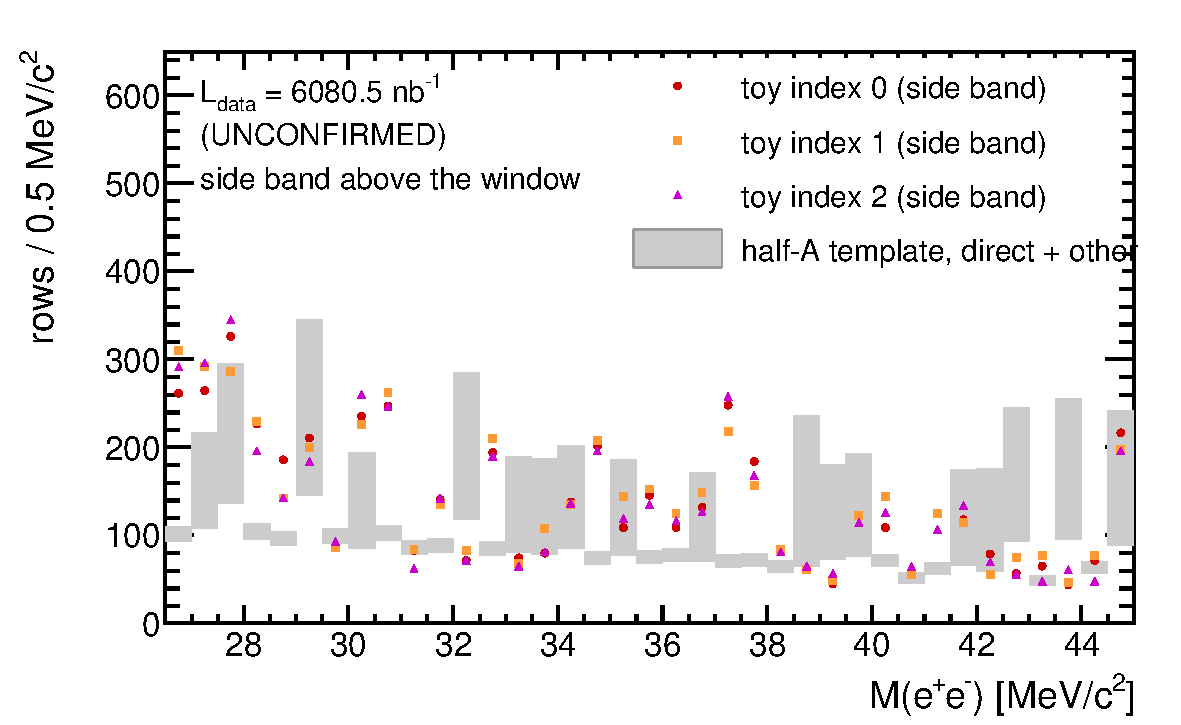
\includegraphics[width=0.75\textwidth]{figs/s5_blind_ana_x17_sideband.pdf}
\caption{\Mee side band (above the X17 window) of three X17 toys against the half-A template
(grey boxes). All toys show the same spikes, which come from single heavy rows of half B.
$\Ldata = 6080.5\,\nbinv$ (UNCONFIRMED).}
\label{fig:s5side}
\end{figure}

\begin{figure}[H]
\centering
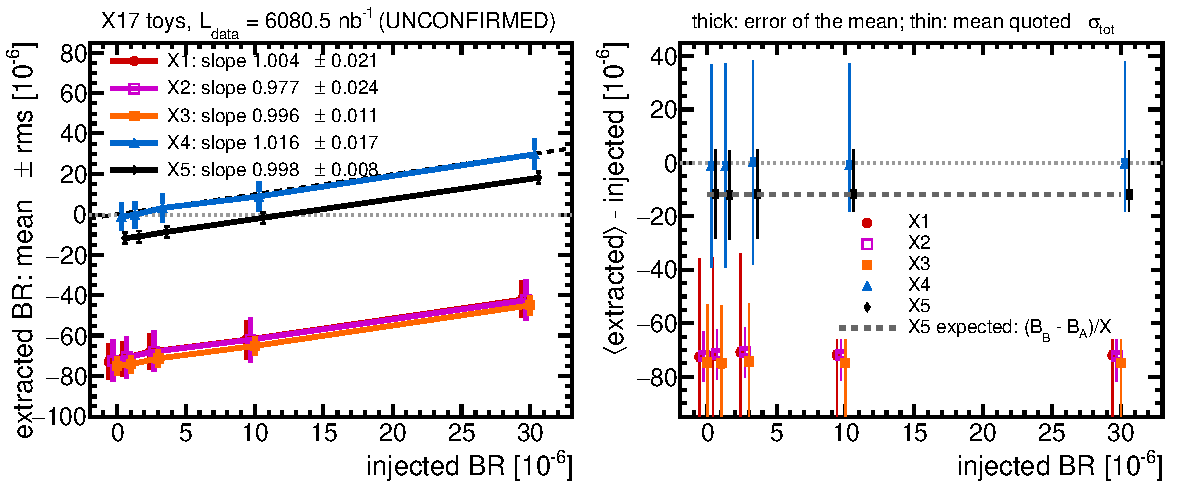
\includegraphics[width=\textwidth]{figs/s5_blind_eval_x17_linearity.pdf}
\caption{Blind test, X17. Left: extracted against injected BR (mean $\pm$ rms over 300 toys) with
straight-line fits. Right: mean offset; thick bars: error of the mean, thin bars: mean quoted
error. Dotted: the offset predicted for X5. $\Ldata = 6080.5\,\nbinv$ (UNCONFIRMED).}
\label{fig:s5x17lin}
\end{figure}

\textbf{Limits of this test.} The test is a closure test inside one model. It does not show how
the methods behave in data.
\begin{itemize}
\item Templates and pseudo-data come from the same SMASH model; there is no CB and no data/SMASH
      shape difference (0.87--1.36 above 0.56\,\GeVcc in earlier comparisons). Template fits are
      favoured by construction. $L_{\mathrm{toy}}$ is 55 times below \Ldata.
\item \textbf{The test was not blind by construction.} The frozen tables that the analyst read
      contain full-sample (A+B) numbers; together with the half-A templates they give the half-B
      truth (for example the PEAK yield 241.4 and the X17 background of half B). No sign was found
      that these numbers were used, and the sealed key was not read before the results were
      written, but the leak was possible.
\item The bootstrap repeats identical rows; how often a row recurs across toys reveals its set and
      therefore class 4 (std) against class 5 ($\eta$ set). This was not exploited, but it is a
      second possible leak.
\item The X17 part used the v1 selection, whose \Mfour window was optimised (partly on a step of
      4 to 8 std rows); the fixed window raises $\mathrm{UL}_{\mathrm{stat}}$ by 3\,\%.
\end{itemize}

%----------------------------------------------------------------------
\subsection{What this means for the data analysis}
\label{sec:s5data}
%----------------------------------------------------------------------
\begin{enumerate}
\item \textbf{Cuts.} In the simulation the four $\eta$-selection cuts remove background outside the
      windows but do not improve the windows themselves; OA$>2^\circ$ and $\alpha_\eta>140^\circ$ cost
      signal (conversions, bump). Their use in data must be justified by the CB and checked there.
      The pion-vertex cuts are the only ones with a gain inside the windows (4--6\,\%); the frozen
      PEAK and DIRECT cuts need the pion track $z$ in the data compact rows, otherwise ``pre + pions
      in vertex fit'' is the alternative.
\item \textbf{Peak extraction.} Template fit (M2) and Gaussian + polynomial with calibration (M1)
      close within a few per cent in simulation; a difference of about 12\,\% between them is normal.
      Linear side bands under the peak lose 20--45\,\% and should not be used.
\item \textbf{Bump.} Side band with the simulated background shape (B4) and template fit; the
      parametric fit tends to be high.
\item \textbf{Direct decay alone.} The split of the peak into class 5 and class 4 is limited by the
      307 std rows of class 4; the quoted error must include the simulation statistics.
\item \textbf{Simulation statistics.} The std set limits the bump and conversion templates
      ($N_{\mathrm{eff}}$ 270--1332) and the X17 background. The common MC error must be added to every
      yield.
\item \textbf{X17.} With the background taken from this simulation the expected limit is about
      $2\times10^{-5}$ (at $\Ldata$ UNCONFIRMED), set by the simulation statistics of the background;
      $5.7\times10^{-6}$ would need the background known exactly. Any X17 estimate must carry the
      background uncertainty in its error. A larger std production or a background determined from
      data side bands would be needed to approach the statistical limit.
\end{enumerate}

\tipbox{\textbf{Open points of this section.} (i) $\Ldata$ is UNCONFIRMED. (ii) The absolute
efficiencies rest on $N_{\mathrm{direct}} = 100\times1\,181\,801$ (representativeness of the 1000
generator files UNVERIFIED). (iii) The X17 \Mpipi distribution and decay angle are assumed
(phase space, isotropic). (iv) The blind test should be repeated with cut definitions only, with
hidden per-toy signal scales and with pseudo-data that do not repeat identical rows; a version with
a CB-like component and a reweighted background shape would test the methods closer to data.
(v) The pion-vertex variables were not compared between simulation and data. (vi) The beam
energy (4530 in the analysis, 4500\,MeV in SMASH) does not affect \Mfour, \Mee and \Mpipi, but does
affect $\mathrm{MM}_4$.}


%======================================================================
\section{Next steps: the data}
\label{sec:next}
%======================================================================
Section~\ref{sec:simres} covered the first four steps of the planned study (signal, acceptance,
cut flow, backgrounds) and tested the optimisation and the signal extraction on simulation. The
next steps use the data:
\begin{enumerate}
\item \textbf{Combinatorial background.} The like-sign method and the factor $k$ from data; the
      signal after subtraction, checked in regions without the $\eta$. Only here can the cuts that
      the simulation finds useless inside the windows (OA, $\alpha_{\mathrm{lab}}$, $\alpha_\eta$)
      show a gain, through the CB.
\item \textbf{Comparison with the simulation} in $\eta$-enriched selections below about
      1\,\GeVcc, with the physics weights of Sect.~\ref{sec:etagen}.
\item \textbf{Signal extraction.} The bump and the peak with the methods that passed the blind
      test (template fit, Gaussian with polynomial; side band with the simulated background shape
      for the bump), with the spread between methods as a systematic error.
\item \textbf{Normalisation.} The ratio of the peak to the bump, in which the luminosity and much
      of the acceptance cancel, gives $\mathrm{BR}(\eta\to\ppee)$ relative to
      $\mathrm{BR}(\eta\to\pipi\piz)\,\mathrm{BR}(\piz\to\ee\gamma)$.
\item \textbf{Systematic errors.} PID cut widths, the opening-angle cut and conversions, vertex
      cuts, the physics weights, the beam energy, the simulation statistics of the templates.
\item \textbf{X17.} The \Mee spectrum in the peak with the background constrained from data, and
      an upper limit.
\end{enumerate}

%======================================================================
\appendix
\section{File locations}
%======================================================================
\begin{tabularx}{\textwidth}{@{}l L@{}}
\toprule
PAT outputs & \code{/hdd3/przygoda/HADES/files/sim/}\allowbreak\texttt{ppee\_\{std,lep,eta\}\_all.root} \\
FAT outputs & \code{/hdd3/przygoda/HADES/FAT_out/sim/}\allowbreak\code{pippimepem_betanew/}\allowbreak\code{output_<set>_<channel>.root} \\
Compact files & \code{.../pippimepem_betanew/scan/sim_compact.root}, \code{sim_compact_eta.root} \\
PID cuts & simulation \code{pp45_pid_cuts_sim_betanew_v6.root},
   experiment \code{pp45_pid_cuts_exp_betanew_v1.root} (PAT repository) \\
PID samples (vae25) & \code{/lustre/hades/user/przygoda/pat3/out/sim/}\allowbreak\code{HADRONS/smash_std_pidsamples/HH_elossfix/},
   \code{.../out/sim/}\allowbreak\code{LEPTONS/smash_std_pidsamples/LEP_merged/} \\
Report macros & \code{docs/latex/macros/}: \code{banana_fill.C} (run on vae25),
   \code{rep_banana.C}, \code{rep_stats.C} \\
\bottomrule
\end{tabularx}

\end{document}
